\documentclass[12pt,letterpaper]{article}

% ── Geometry ──────────────────────────────────────────────────────────
\usepackage[margin=1in,headheight=14pt]{geometry}

% ── Fonts (XeLaTeX) ──────────────────────────────────────────────────
\usepackage{fontspec}
\setmainfont{DejaVu Serif}
\usepackage{xeCJK}
\setCJKmainfont{Noto Serif CJK SC}

% ── Spacing ──────────────────────────────────────────────────────────
\usepackage{setspace}
\onehalfspacing
\usepackage{parskip}

% ── Math ─────────────────────────────────────────────────────────────
\usepackage{amsmath}
\usepackage{amssymb}
\usepackage{unicode-math}

% ── Tables ───────────────────────────────────────────────────────────
\usepackage{booktabs}
\usepackage{longtable}
\usepackage{array}
\usepackage{multirow}
\usepackage{calc}

% ── Figures ──────────────────────────────────────────────────────────
\usepackage{graphicx}
\usepackage{float}
\usepackage[section]{placeins}

% ── Captions ─────────────────────────────────────────────────────────
\usepackage[font=small,labelfont=bf]{caption}

% ── TOC / LoF / LoT layout: widen page-number column for three-digit page
%    numbers and widen the subsection-number slot for multi-digit labels.
\makeatletter
\renewcommand{\@pnumwidth}{2.5em}
\renewcommand{\@tocrmarg}{3.5em}
\renewcommand*\l@subsection{\@dottedtocline{2}{1.5em}{3.0em}}
\renewcommand*\l@subsubsection{\@dottedtocline{3}{4.5em}{3.8em}}
% Widen the section-number slot in the TOC from the article-class default
% 1.5em to 2.0em so two-digit section numbers (10–16) have the same
% horizontal gap before the title as single-digit numbers do.
\renewcommand*\l@section[2]{%
  \ifnum \c@tocdepth >\z@
    \addpenalty\@secpenalty
    \addvspace{1.0em \@plus\p@}%
    \setlength\@tempdima{2.0em}%
    \begingroup
      \parindent \z@ \rightskip \@pnumwidth
      \parfillskip -\@pnumwidth
      \leavevmode \bfseries
      \advance\leftskip\@tempdima
      \hskip -\leftskip
      #1\nobreak\hfil \nobreak\hb@xt@\@pnumwidth{\hss #2}\par
    \endgroup
  \fi}
\makeatother
\setcounter{tocdepth}{2}

% Suppress \paragraph titles from appearing in the TOC.
% Some package interaction (likely titlesec) writes paragraph entries
% regardless of tocdepth; redefining \l@paragraph as a no-op silences them.
\makeatletter
\renewcommand*\l@paragraph[2]{}
\makeatother

% ── Headers ──────────────────────────────────────────────────────────
\usepackage{fancyhdr}
\pagestyle{fancy}
\fancyhf{}
\fancyhead[L]{\small\itshape Pagadala}
\fancyhead[R]{\small\itshape The Long Childhood}
\fancyfoot[C]{\thepage}
\renewcommand{\headrulewidth}{0.4pt}

% ── Colors and hyperlinks ─────────────────────────────────────────────
\usepackage{xcolor}
\usepackage[colorlinks=true,linkcolor=blue!60!black,citecolor=blue!60!black,urlcolor=blue!60!black,
  pdftitle={The Long Childhood: On the Convergence of Humanity},
  pdfauthor={Krishna Pagadala}]{hyperref}

% ── TikZ (mechanism diagram) ─────────────────────────────────────────
\usepackage{tikz}
\usetikzlibrary{arrows.meta, positioning, calc, decorations.markings}

% ── Code / script references ─────────────────────────────────────────

% ── Prevent overfull lines ───────────────────────────────────────────
\tolerance=1000
\emergencystretch=3em

% ── CSQuotes for proper quoting ──────────────────────────────────────
\usepackage{csquotes}

% ── Section formatting ───────────────────────────────────────────────
\usepackage{titlesec}
\titleformat{\section}{\Large\bfseries}{\thesection.}{0.5em}{}
\titleformat{\subsection}{\large\bfseries}{\thesubsection}{0.5em}{}
\titleformat{\subsubsection}{\normalsize\bfseries}{\thesubsubsection}{0.5em}{}

% ══════════════════════════════════════════════════════════════════════
% DOCUMENT
% ══════════════════════════════════════════════════════════════════════

\begin{document}

% ── Title ─────────────────────────────────────────────────────────────
\begin{titlepage}
\begin{center}
\vspace*{2cm}
{\LARGE\bfseries The Long Childhood\par}
\vspace{0.5cm}
{\large\itshape On the Convergence of Humanity\par}
\vspace{1.5cm}
{\large Krishna Pagadala\footnote{Software engineer of twenty-five years' practice, self-taught in the substantive literatures over the same period; the framing tested here emerged across it (see \S\ref{why-the-mechanism-has-been-missed}). \url{https://educationfirst.world}}\par}
\vspace{0.5cm}
{\normalsize\itshape July 2026\par}
\vspace{1cm}
{\small\itshape In memory of Richard A.\ Easterlin (1926--2024), who asked the right question.\par}
\vspace{0.5cm}
{\small\itshape In memory of Jane Goodall (1934--2025), who saw what the juvenile dependency period does.\par}
\vspace{0.5cm}
{\small\itshape In memory of Mahbub ul Haq (1934--1998), who knew that people are the real wealth of a nation --- and left one step for the rest of us.\par}
\vspace{1cm}
\end{center}

\begin{abstract}
\noindent Humans have the longest juvenile dependency of any species
--- nearly two decades of plastic brain growth embedded with adult
teachers. This window is the channel through which one generation
installs a cognitive architecture in the next deep enough to use,
extend, and transmit. Wallace's theory explained how species
differentiate under isolation; I document the inverse --- what one
species has done with its window, post-1960, at population scale. By
2022, 154 countries --- across every political system and
continent --- have crossed a shared developmental threshold:
fertility below 3.65 births per woman and life expectancy above 69.8
years (the 1960 United States values) --- the crossing itself. The
convergence is the population-scale signature of loading schooling
into the long childhood; its absence is the signature of failing to
do so. More broadly, the outcomes I predict the mechanism moves ---
fertility, longevity, offspring survival --- are the classical
fitness components of life-history theory; this convergence is the
event I predict and explain. I address the
crossing event in the post-decolonization window and its generational
predictor; pre-transition local fertility patterns and post-crossing
trajectory dynamics are outside my scope.

What is uniquely human is cultural transmission applied to tools
that rebuild the environment, and to the specialisation of
individuals across them. Fire was the first; agriculture, metallurgy,
literacy, and medicine followed --- each a culturally-transmitted
tool that manipulates the environment at a scale no individual could
invent alone. Formal schooling is the latest and highest-bandwidth
payload ever delivered through this evolved channel; the convergence
is what that delivery produces.

I argue that education is necessary and sufficient for convergence
at population scale. \textbf{Necessity:} of
the 154 countries that have crossed, every one through mass
schooling. \textbf{Sufficiency:} every country that reaches the
educational threshold crosses, at a pace set by state priority ---
one generation (\textasciitilde28 years) under singular-priority
expansion, two to three generations (\textasciitilde60 years) under
competing-priority expansion, never under no-priority regimes.
Sufficiency holds because an educated population operates every
other policy lever at policy speed --- adopting new institutions,
rewriting rules, taking up new technologies --- while an uneducated
population cannot, no matter how good the rules layer is.
Institutions, markets, and rules are bounded by the education of the
population that builds and uses them
(Section~\ref{education-as-limiting-factor}). But education
\emph{produces} longevity and fertility outright, while it only
\emph{bounds} income --- markets can be held below what an educated
population would build --- which is why the definition keeps the first
two and drops income (Section~\ref{defining-development}). Because
the transmission operates through the \emph{home niche} --- the
near-older humans embedded in the child's daily life across the
juvenile dependency window --- the one-generation floor is biological
(the turnover time), not policy-responsive. An educated home niche carries norms, health
behaviours, and the expectation of school completion forward to
children who exercise these as household decisions a generation later.

At the household scale the claim is concrete: a household whose
parents have completed lower secondary is a developed household, and
a developed country is one in which enough households have crossed
this parental threshold. The 185 countries (1950--2015), of which 144 are observed
during their lower-secondary transition (the expansion sub-panel:
1975--2015 country-years where child-year completion sits in
$[10\%, 90\%]$), span four generational depths --- one century ---
and bear the mechanism out. A great-great-grandparent's school completion
predicts their great-great-grandchild's child-survival outcomes a
century later.
Six empirical signatures are deduced from the biology
--- generational timing, multi-generational persistence, asymmetric
disruption, income independence, universality, collective action ---
and tested against the panel; all six hold. The identification is biological and
natural-experimental; the cross-country panel is the population-scale
evidence that bears out those predicted signatures across the whole species.

Easterlin (1981) identified mass schooling as the cause of uneven
development and asked why the whole world wasn't yet developed; his
answer was largely set aside while the field pursued institutions,
geography, and factor accumulation. Tested on its own terms with the
field's own methods, the alternative collapses: log GDP per capita's predictive
power decays within a single generation, and once education's
contribution is residualized out, GDP predicts nothing. Provision
without educated populations produces no durable outcomes.
Institutions are built by educated populations, not the reverse.

\vspace{0.5em}
\noindent\textbf{Keywords:} life-history theory; extended juvenile
dependency; fitness components; vertical cultural transmission;
developmental niche construction; cultural-transmission niche; home
niche; literate cultural transmission; generational lag; mass
schooling; convergence; human development; demographic transition
\end{abstract}

\thispagestyle{empty}
\end{titlepage}

\newpage
\tableofcontents

\newpage
\listoffigures

\newpage
\listoftables

\newpage

\section*{How to Read This Paper}\label{how-to-read}

Two readers are intended. The first is the policy maker who must act
today: the ministry official, the foundation programme officer, the
multilateral staff member who allocates finite political and fiscal
capital between competing priorities and needs to know what the
evidence requires of that allocation.

The second is the scholar who reads this as a primary text long after
the present arguments have ceased to matter --- the reader for whom
this is one document in the record of how a species came to recognise
the channel through which it became what it is.

Neither reader is served by a single linear path through a long
argument. The policy maker drowns; the second reader finds the
structure inferable but not declared. This guide is the declaration.
Four entrances are offered. Three are organised by the discipline the
reader arrives from; the fourth is for the reader whose first question
is where the work came from. Each traverses the same argument; the
difference is the order of approach and which sections carry the load.

\textbf{From biology.} The species-level claim is established in
Sections~\ref{longest-juvenile-dependency} (the eighteen-year juvenile
dependency), \ref{cultural-transmission} (cumulative cultural
transmission and the tools that rebuild environments),
\ref{education-as-payload} (formal schooling as the highest-bandwidth
payload through the channel), and \ref{generational-transmission-and-state} (the state as the
agent that paces the channel).
Sections~\ref{natural-experiments} and \ref{country-histories} are
the mechanism running in observable time --- famines, regime
collapses, and country trajectories where the channel is severed,
held fixed across institutional variation, or pushed at maximum
speed. Section~\ref{hollow-education} tests it in the negative:
Soviet-bloc schooling, credentialed but hollowed of real content,
did not produce development --- the predicted outcome if the channel
is real. The 185-country panel from Section~\ref{the-panel}
onward is the population-scale signature of the life-history claim;
the biologist may read it as the signature without engaging the
regression apparatus that demonstrates it to readers from other
disciplines.

\textbf{From human development.} Section~\ref{the-convergence} fixes
the developmental threshold in the tradition of Mahbub ul Haq and Amartya Sen, who
already did the philosophical work of dethroning income.
Section~\ref{natural-experiments} is the natural experiments,
Section~\ref{country-histories} is the country trajectories,
Section~\ref{the-panel} is their population-scale signature, and
Section~\ref{hollow-education} is the falsification: hollow Soviet
schooling that did not develop confirms the channel by the negative case.
Section~\ref{what-every-framework-was-reaching-for} is the engagement with
Smith, Deaton, and the institutional alternative --- and Sen and Drèze's
frame read one layer deeper.
Section~\ref{why-the-loading-in-childhood-is-invisible} diagnoses why
the human-development apparatus treats education as one competing
priority among many rather than the substrate the rest sit downstream
of, and Section~\ref{why-it-was-never-chosen} why the households
who would gain most could not choose it either.
Section~\ref{the-decision} is what the path is for.

\textbf{From the decision today.} The reader who must allocate this
quarter may begin at Section~\ref{the-prediction} (the six
signatures I require of the data), proceed through
Sections~\ref{natural-experiments} and \ref{country-histories} (the
natural experiments that do the identification work the panel alone
cannot, and the country trajectories closest to the reader's
situation), then Sections~\ref{the-panel} and~\ref{hollow-education}
(the universal panel test and the Soviet hollow-education
falsification). Section~\ref{the-decision} is the operational
claim. Appendix~\ref{appendix-reproducibility} points the reader to the
full reproducibility stack (scripts and 20-test econometric battery
on GitHub) for satisfying a technical audience before acting.
Sections~\ref{the-dark-parallel}--\ref{convergence-and-peace} are
optional for the operational reader; they argue the same decision
delivers peace, but the operational instruction at
\S\ref{the-decision} stands without them.

\textbf{From the question of warrant.} The reader whose first question
is where this came from --- before what it claims --- may begin at
\S\ref{why-the-mechanism-has-been-missed} (how the framing emerged, on
what data, across what period) and the Acknowledgments (the
intellectual lineage the synthesis was built from, and the
AI-assistance disclosure). The rest of the paper is then read against
a synthesis whose origin and method are already disclosed.

\textbf{Across all paths.} The evidence runs in two tiers of history, one falsification, and one species-scale panel. The deep history (Chapters~\ref{longest-juvenile-dependency}--\ref{generational-transmission-and-state}) --- evolutionary anthropology --- establishes the mechanism: what humans are, why the juvenile dependency window admits a payload no other species can carry. The recent history (Chapters~\ref{natural-experiments}--\ref{country-histories}) --- the natural experiments and the country histories --- shows the mechanism running in observable time. The hollow-education falsification (Chapter~\ref{hollow-education}) tests it in the negative: schooling without real content does not produce development, as the Soviet anomaly shows. The 185-country panel (Chapter~\ref{the-panel}) sharpens that pattern at the scale of the whole species, in the regression form an economics reader requires; it shows the pattern is universal across the species --- the population-scale evidence that supports what the biology and the histories establish. These are not one method applied many times but several pointed from different directions --- deduction from the biology, comparison across natural experiments and country histories, falsification from the Soviet anomaly, regression across the panel. The proof is biological; that the others converge on the same channel, none of them able to see the assumptions of the rest, is why I trust it is the channel and not an artifact of how I looked.

This paper is written for readers who want to evaluate the evidence directly. No specialised training is required to read this.

The argument is one argument. The paths are entrances, not parts. A
reader who follows only one entrance will see less than is here. A
reader who must act this quarter should follow the third path and
accept that the first two are why the third holds.

\newpage

\section*{Glossary}\label{glossary}

I use several specialised terms drawn from evolutionary
anthropology, cultural-transmission theory, and demographic
analysis. Each is defined below with a section anchor for its
load-bearing use.

\renewcommand{\arraystretch}{1.15}
\begin{longtable}{@{}p{0.27\textwidth}p{0.69\textwidth}@{}}
\toprule
\textbf{Term} & \textbf{Definition} \\
\midrule
\endhead

Long childhood / Juvenile dependency window &
The roughly eighteen-year period of plastic brain growth during which
the human is dependent on adult caregivers --- the longest juvenile
dependency of any species. The substrate every other term in this
glossary loads into
(Section~\ref{the-dependency-window}). \\

Agency transfer &
The threshold at roughly age fifteen --- and for many individuals a
year or two later --- at which the cognitive architecture absorbed
during the long childhood becomes the learner's own operating system
rather than the parents' to direct. The window remains open until
roughly eighteen; agency transfer is the milestone inside it
(Section~\ref{the-threshold-of-agency-transfer}). \\

Cultural-transmission (CT) niche &
The set of near-older humans embedded in a child's daily life across
the eighteen-year juvenile dependency window --- parents,
grandparents, older siblings, near-kin, and the surrounding adults
of the cooperative-breeding unit (Hrdy 2009): teachers, neighbours,
and other community alloparents. Channel and content are
inseparable: the near-adults \emph{are} the transmission
(Chapter~\ref{cultural-transmission}). \\

Home niche &
The CT niche carried by the household. Symmetric: it transmits
whichever CT regime --- literate or illiterate --- it inherits
(Section~\ref{the-generational-transmission-mechanism}). \\

School niche &
The CT niche constructed by the state through schools, teachers, and
curriculum. Adds a second niche alongside the home niche during the
transition (Section~\ref{the-state-reach-not-mechanism}). \\

Home-niche modulation &
The home niche conditions how much of the school niche a child can
absorb. Fully illiterate home niches give no scaffolding; literate
home niches compound with school
(Section~\ref{the-generational-transmission-mechanism}). \\

Categorical literacy (Level 1) &
The categorical reorganisation of the individual brain that formal
schooling produces. Literate and pre-literate cognition differ in
kind, not degree
(Section~\ref{categorical-brain-reorganisation}). \\

Literate CT (Level 2) &
The categorical regime change at the society scale: cultural
transmission itself comes in two incomparable forms. Literate CT
enables non-kin coordination at population scale; illiterate CT
does not, no matter how long it runs
(Section~\ref{literate-ct}). \\

Human ratchet &
Each generation's schooled cohort becomes the next generation's home
niche, raising absorption of the next school niche the state
delivers. Self-amplifying, one-way, state-paced
(Section~\ref{the-human-ratchet}). \\

Generational cycle (\textasciitilde 28 years) &
The cohort-replacement interval --- the time from one generation's
schooling to the next's, parent cohort to child cohort, both measured
at ages 20--24. Its empirical anchor is the cohort-weighted mean age
at childbearing ($\overline{\mathrm{MAC}} = 28.8$ years across the
expansion-phase panel), and it is the biological basis for the paper's
headline $T{-}28$ lag. It is distinct from agency transfer (the
\textasciitilde 15-year milestone inside the dependency window,
above): the cycle is how long the cohort schooled under one click of
the ratchet takes to become parents themselves, not the age at which a
child becomes an agent. Country-aggregate crossing time is
compositional and depends on the starting baseline
(Section~\ref{country-histories}). \\

$\beta_g$ &
Generational amplification coefficient: the within-country slope of
child lower-secondary completion on parental completion at the
one-generation lag, with country fixed effects. A one-pp rise in
the parental cohort predicts a $\beta_g$-pp rise in the child cohort.
Exceeds 1 at low baselines (the school niche extends reach above
what the home niche alone carries); approaches 0 at high baselines
(ceiling compression). The headline panel is post-1975, 144 countries
in the expansion window $[10\%, 90\%]$
(Table~\ref{tab:cutoff}); a long-run 1900--2015 panel on a
28-country subsample with self-determined education policy
shows the same pattern at
deeper baselines, where the post-1975 panel is weighted toward
countries already approaching the ceiling. Per-country 28-year sliding windows
(Figure~\ref{fig:beta-baseline}) trace the within-country trajectory. Same
regression specification, three samples. \\

Four radii of educational effect &
Self and children (action), close relatives (action), polity
(political pressure), humanity (talk). Each is a boundary draw of
the same coalitional in-group mechanism (Tooby \& Cosmides 2010);
potency falls as the boundary widens
(Section~\ref{from-action-to-talk-how-education-reaches-beyond-the-household}). \\

Three state regimes &
No priority, competing priority, singular priority. The state's
choice sets the pace at which the school niche reaches the home
niche (Section~\ref{the-state-reach-not-mechanism}). \\

Hollow education &
School systems where reported completion runs ahead of cognitive
depth, so the certificate is real but the literate-CT regime has not
flipped. The Soviet republics 1960--1990 are the paper's headline
case; convergence lags
(Chapter~\ref{hollow-education}). \\

\bottomrule
\end{longtable}\addtocounter{table}{-1}% undo longtable's auto-step (we use manual \refstepcounter for labels)

\newpage

\section{The Convergence}\label{the-convergence}

Human childhood is the channel through which each generation
transmits itself to the next. It has never been empty. Filling it
with education is what makes a population developed. That is my
argument.

Education is fundamental to human well-being. Not important ---
fundamental. The distinction matters. Important means high on a list.
Fundamental means the list does not exist without it.

Between 1960 and 2022, 154 countries crossed the two thresholds
that define human development --- the United States values of 1960
(formalised in \S\ref{defining-development}). The crossing is what
one species does when it loads its long childhood --- the
eighteen-year juvenile dependency window --- with formal schooling at
population scale. Figure~\ref{fig:cum-share} traces the accumulation. The
share of humanity living in a developed country climbs slowly from
13\% in 1961 to roughly 20\% by 1993, jumps when China crosses in
1994, passes 50\% in 2001, and reaches 80\% by the late 2010s. Four
in five people now live in a developed country --- one species,
across every political system and every continent, converging onto a
single developmental threshold.

This convergence is the paper's empirical anchor. What varies between
countries is the speed of arrival. Spain had wealth, an empire, and
global power; Korea in 1953 had none of them. Spain took
four-hundred-and-fifty years; Korea took thirty-five. Same juvenile
window, same species, same biology. What separated them was the decision to
extend schooling.

I state the claim in the form that can be broken. Loading the long
childhood with schooling is necessary and sufficient for development at
population scale. Necessary: of the one-hundred-fifty-four countries that
have crossed, every one crossed through mass schooling. Sufficient: every
country that has reached the schooling threshold has crossed, at a pace the
state sets but cannot escape. Put this way, the claim hands you its own
falsifiers. A country that crosses both demographic thresholds with its
young adults still below the schooling floor breaks the necessity. A
country that reaches the floor, expands undisrupted, and has not crossed a
generation later breaks the sufficiency
(Chapter~\ref{the-prediction} states both bets in numbers --- the floor
near 35\%, the limit near thirty years). Wallace explained how one species
becomes many when a barrier divides them; I document the inverse --- many
becoming one as a single payload reaches all of them --- and I have named
the two observations that would prove it wrong. The same channel carried
religion for millennia and divided rather than converged, because identity
payloads are selected for incompatibility while utility payloads are
culture-invariant --- there is no Hindu calculus. Convergence is what the
channel does when the payload is utility.

A single cause reads as a weakness; here it is the prediction. A universal
outcome demands a shared cause: the 154 countries that have crossed, across
every regime and continent, cannot have converged on anything that differs
between them. Strip away everything that does and education is what remains
--- residualize it out and income predicts nothing
(Chapter~\ref{the-panel}). The convergence is the signature of one cause,
not evidence against it.

I argue that the mechanism is biological. Humans alone have
a juvenile dependency period long enough --- nearly two decades of
plastic brain embedded with dedicated adult teachers --- for cultural
transmission to load the population with knowledge deep enough to
produce the convergence (Konner 2010; Hrdy 2009). The pace of that
loading is not administrative but biological: it is set by demographic
metabolism (Lutz 2013), the rate at which more-schooled cohorts
replace less-schooled ones (Section~\ref{education-as-limiting-factor}).
Formal schooling is the latest and highest-bandwidth payload ever
delivered through that channel. Once an educated population is in
place, development is no longer a policy target pursued through a
list of interventions; it is the population's own expression of
what the juvenile dependency window permits. Chapters~\ref{longest-juvenile-dependency} through
\ref{generational-transmission-and-state} establish the biology.
Chapter~\ref{the-prediction} states the predictions the deep history
entails. Chapter~\ref{the-panel} renders the pattern as a 185-country
universe with the regression sample restricted to the 144-country
expansion sub-panel --- universal across regimes and continents.
Chapters~\ref{natural-experiments} and \ref{country-histories} are the
recent history --- natural experiments and country trajectories where
the mechanism is observable in time.
Chapters~\ref{the-dark-parallel}--\ref{convergence-and-peace} extend
my argument forward.
Chapter~\ref{what-every-framework-was-reaching-for} takes up the frameworks the
biological claim explains;
Chapter~\ref{why-the-loading-in-childhood-is-invisible} diagnoses why all of them
miss the substrate at once, and Chapter~\ref{why-it-was-never-chosen} why,
even seen, it was never chosen. Chapter~\ref{the-decision} states what
remains: the decision that no policy calculation dispenses from.
Figure~\ref{fig:spine} traces the path the rest of the paper defends.

By ``education'' I mean the educated population, not the
school system. The school system is the delivery mechanism; the
educated adult is the operative unit. A country can rebuild schools
within a decade; it cannot rebuild an educated population in less than
a generation (Cambodia,
Section~\ref{cambodia-the-home-niche-shadow}). The mechanism --- the home
niche, the school niche, and the state extending one to reach the
other --- is in
Chapter~\ref{generational-transmission-and-state}.

\begin{figure}[p]
\centering

\includegraphics[width=\textwidth]{figures_web/fig_chain.png}\\[1.6ex]

\includegraphics[width=\textwidth]{figures_web/loading_by_priority.png}
\caption[The argument in one path]{The argument in one path, and the
priority that paces it. \emph{Top:} what a loaded childhood produces ---
categorical literacy, the household decisions educated adults make, and
the fall in fertility and the rise in life
expectancy that follow. The schooled child grows up to be a parent, and
loads their own children's childhood; the ratchet turns once a
generation. Income is a
by-product of the same educated population, not a separate channel to
development (Section~\ref{gdp-has-no-independent-effect}).
\emph{Bottom:} the same window, loaded at different speeds. Under
singular priority Korea reaches near-universal lower-secondary
completion within a generation; under competing priorities India climbs
slowly; Spain, a sovereign power that did not prioritise, sits at zero
across the nineteenth century (its first observed cohort completes
lower secondary at essentially zero, and completion rises only
thereafter). Loading the window is necessary and sufficient for the
crossing; the state sets only the pace.}
\label{fig:spine}
\end{figure}

\subsection{Defining Development}\label{defining-development}

I define a country as developed when it has simultaneously achieved a
\textbf{total fertility rate (TFR) below 3.65} and \textbf{life
expectancy (LE) above 69.8 years} --- the 1960 United States values (World
Bank WDI).

These two measures are chosen because they are intrinsically valuable
--- not as proxies for something else, but as the things themselves.
The UN's Human Development Index (UNDP 1990) already treats health
and education as intrinsically valuable alongside income. This
definition takes that logic to its conclusion: it retains the two
outcomes that are ends in themselves and drops the one that is not.

Life expectancy is the most fundamental measure of human welfare.
Every other outcome --- income, freedom, knowledge, dignity ---
presupposes being alive. A country where people die at 45 has failed
on the most basic term, regardless of its GDP or institutional
quality. Life expectancy is not one metric among many; it is the
precondition for all others.

The number of children a woman bears defines the shape of her entire
adult life in ways that no other variable does. Seven children means
two decades of continuous pregnancy and nursing, followed by a further
decade of child-rearing before the last child is self-sufficient
(Section~\ref{demographic-structure-and-the-fertility-transition}).
The difference between seven children and two is not incremental; it
is the difference between a life fully absorbed by reproduction and a
life in which the education already received has room to be used --- in
work, civic participation, or rest.

These are also the two most direct population-level expressions of
whether the cognitive transformation produced by education has
occurred. Life expectancy tracks whether people have the planning
horizon, health knowledge, and behavioural capacity to sustain their
own survival. TFR tracks whether women have moved from biological fate
to conscious reproductive choice --- precisely the cognitive autonomy
that underlies every other dimension of human flourishing.

Hans Rosling's Gapminder (Rosling 2018) plotted every country's
path on the TFR--life-expectancy plane and dissolved the two-box
``developing vs developed'' framing: populations travel together
along a single diagonal, from high fertility and short life to low
fertility and long life. The two-threshold definition used here pins Rosling's
diagonal to a specific point: the position occupied by the 1960
United States. Rosling's own account of what drives the movement was
multivariate; I argue one variable does it: education.

Every competing metric of development is either a component of life
expectancy and fertility --- child mortality is a component of LE,
nutrition is a cause of LE variation, sanitation prevents child death
that shows up in LE --- or a consequence of the cognitive
transformation that moves them (institutional quality, income,
democracy). A part can't outrank the whole. An effect can't outrank
its cause. LE and TFR are not the best items on a list of
development metrics --- they are what the list is measuring.

No country considered developed --- by any definition, under any
framework --- has life expectancy below 69.8 or TFR above 3.65.

For readers who treat income as the goal of development: excluding
it costs nothing empirically --- education predicts GDP per capita
as strongly as it predicts LE and TFR (Table~\ref{tab:edu-outcomes}).
Crossing dates under three threshold specifications shift by 10--30
years but the ordering holds; countries with high expansion rates
cross any threshold within 14--16 years. I exclude income from the
outcome anyway, because measuring development through income would
assume the answer: GDP is one of the variables competing to explain
LE and TFR, and folding it into the outcome would let it carry the
result by definition rather than by evidence. Excluding it is the
harder test, not a way around a weaker one.

The exclusion has a mechanical basis, not only a methodological one.
Education produces longevity and fertility outright: a loaded
population runs its own health and schooling, so the two outcomes
follow under any political system. Income it only bounds --- markets
an educated population can build but a political system can suppress,
so education is necessary for income without being sufficient for it.
The definition keeps what education produces and drops what it merely
bounds.

Why the 1960 USA? It is the natural baseline: 1960 marks the start of
mass decolonization, and the USA was the unambiguous global hegemon.
A country that crosses both thresholds has surpassed the richest
nation on earth on the metrics that matter for human welfare. The
USA in 1960 was mid-transition --- its TFR of 3.65 was the baby boom
peak, and it did not complete its own fertility transition until
1972. A TFR below 3.65 is itself an achievement: in 1960, only the
developed world --- Europe, Japan, and a few settler states, roughly
a quarter of humanity --- had fertility that low. The remaining
three-quarters of humanity averaged a TFR above 6 --- the human
baseline.

The countries that had already crossed both thresholds by 1960 were
those with the longest prior histories of mass education: Scandinavia,
the Netherlands, France, Switzerland, the United Kingdom, Australia,
and New Zealand. Japan --- despite a TFR of 2.0 --- had life
expectancy of 67.7, just below the threshold; it crossed in 1964. By
2022, 154 countries are developed by this definition --- four in five
people on earth, 80\% of humanity, now live in a developed country.
Figure~\ref{fig:cum-share} traces this accumulation over time.

\begin{figure}[htbp]
\centering
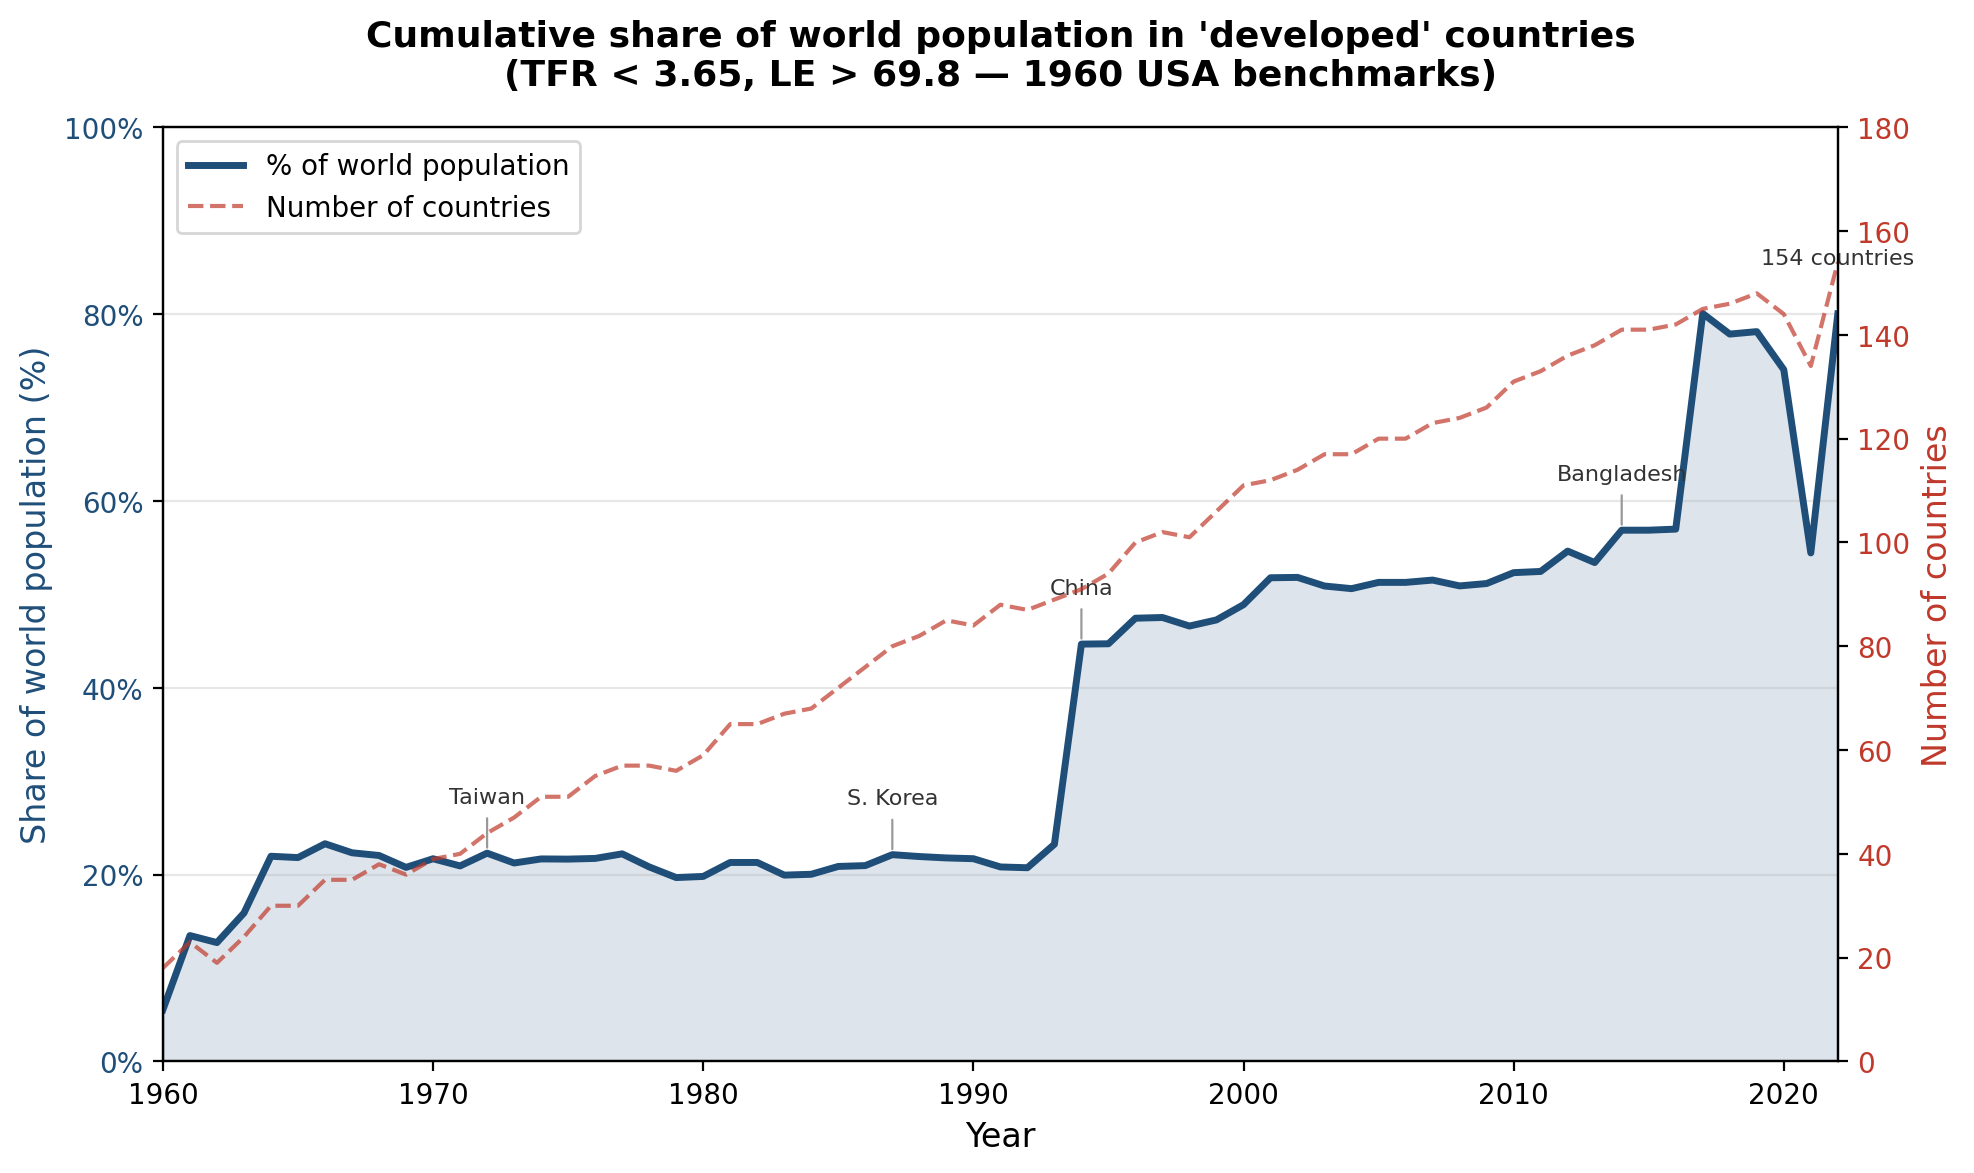
\includegraphics[width=\textwidth]{figures/cumulative_developed.png}
\caption[Cumulative share of world population crossing both development thresholds, 1960--2022]{Cumulative share of world population crossing both
development thresholds (TFR \textless{} 3.65, LE \textgreater{} 69.8),
1960--2022. Slow climb from 13\% (1961) to \textasciitilde20\% (1993);
vertical jump in 1994 when China crosses; 50\% by 2001; 80\% by
2017--2022. \emph{(Source: World Bank WDI, WCDE v3.)}}
\label{fig:cum-share}
\end{figure}

\subsection{What the Convergence Requires}\label{what-convergence-requires}

Two intellectual traditions --- one asking what development is, the
other asking what humans are --- converge on the same mechanism.

In development economics, Haq and Sen broke the identification of
development with income when they built the Human Development Index
(UNDP 1990). Sen's capabilities framework (1999) made explicit that
what matters is what people can do and be, not what they earn --- and
he pointed to Kerala, Sri Lanka, and China as the right anomalies,
welfare outcomes far above what their incomes predicted. Easterlin
(1981) identified mass schooling as the binding constraint and asked
why it had not reached the whole world. Lutz and Kebede (2018) showed
that the income--life-expectancy relationship tightens when education
replaces income on the horizontal axis. The income--mortality link
was education proxying through income all along.

The Human Development Index (UNDP 1990) registered this without
naming it. Haq and Sen could have placed any indicator alongside
life expectancy and income --- sanitation, calories, freedom indices,
infrastructure, institutional quality --- and chose education. The
choice predates the panel evidence by three decades; they reached it
by induction from the cases they could see. I supply the
mechanism the choice was already tracking: education is co-equal
with health and income on the index because it is upstream of both,
and because it is the only input that meets the structural criterion
(\S\ref{education-as-limiting-factor}).

In evolutionary biology, Konner (2010) documented that the human
juvenile dependency is the longest of any species --- roughly
eighteen years of plastic-brain exposure to dedicated adult
transmitters, most of it observational rather than formal; schooling
is a late, high-bandwidth intensification of the same channel. Hrdy
(2009) showed that a dependency this long was only viable because
humans evolved as cooperative breeders: mothers, fathers,
grandparents, older siblings, and alloparents share the burden of
provisioning children that no pair of parents could carry alone. The
household I measure is the one Hrdy identifies. Boyd and
Richerson (1985) formalised parent-to-child cultural transmission as
the mechanism by which human populations accumulate knowledge across
generations --- at higher bandwidth than the genetic channel, because
transmission is continuous across the dependency window rather than
a single reproductive event. Maynard Smith and Szathmáry (1995)
set this channel in the deepest available frame: the origin of human
language and culture is the last of the major transitions in
evolution, and every such transition is a change in how heritable
information is stored and transmitted. They separate limited
hereditary systems, which carry only a small fixed set of states,
from unlimited ones, whose possible messages grow combinatorially
without bound --- the genetic code is the first unlimited system, and
language is the second, open-ended for the same reason, because the
mapping from sign to meaning is arbitrary rather than fixed by
physics. Culture became heritable in the strong sense when this
second unlimited system began running on top of the first. That is
what the higher bandwidth names precisely: not a faster genetic
channel but a categorically larger one, and the long childhood is the
transmission window wide enough to load it. And this locates the
convergence itself. Every major transition before it worked by changing
the substrate of heredity --- molecules bound into chromosomes, cells
into the eukaryote, solitary individuals into the multicellular body,
and, at the origin of language, a second inheritance system laid over
the genetic one. The convergence of the species into a single
developmental state is the next move in that sequence, and the first to
leave the substrate untouched: it changes what the species is --- how
long it lives, how many children it has, the age at which they die, the
scale at which it cooperates --- and alters not one base of the genome.
The genome of a developed population and an undeveloped one is
identical; the whole of the difference is the payload loaded through the
long childhood. This is why a crossing that genetic change would need
millennia to make can be made in a single generation --- Korea in
thirty-five years --- because it is a change in the content of the
second inheritance system, not in the hardware of the first. Wallace's
mechanism divides one species into many along the genetic channel; this
transition draws the many together along the cultural channel --- a
substrate that mechanism never touches. Hawkes (2003) closed the loop:
post-reproductive human longevity, unique among primates, evolved to
support grandchild survival, which is why longevity and fertility
move together as one developmental signature.

These findings form a chain. Hamilton (1964) formalised inclusive
fitness: behaviour that raises the reproductive success of kin is
selected even when it lowers the actor's own. Boyd and Richerson
extended the logic from genes to culture: knowledge, norms, and the
decision to educate are themselves heritable and subject to the same
selective pressures, with the adults embedded in the child's daily
life the highest-fidelity route. The home niche is inclusive fitness
operating through cultural rather than genetic inheritance ---
kin-directed investment in descendants, carried by the extended
juvenile dependency period and supported by the post-reproductive
longevity that evolved alongside it.

Kin selection and the channel are gated on different things, and the
difference, I claim, is the whole reason mass schooling works.
Inclusive fitness explains why a transmitter is \emph{motivated} to
load a child --- parents invest in their own descendants. It does not
explain who is \emph{able} to. The payload channel is gated not on
descent but on being the same species: every human child ships with
the same language-ready brain, so any loaded adult can load any
child, kin or not. Blood sets the motive; species sets the reach.
This is why the alloparents already in the niche --- teachers,
neighbours --- can transmit at all, and why a state can carry a
generation across whose own parents never crossed, by placing loaded
conspecifics where the household has none. It also fixes the
bandwidth into a single child. Genetic inheritance has a fan-in of
exactly two, the child's two parents; the cultural channel's fan-in
is every loaded near-adult the child can reach --- which is why the
developmental shield is a property of the community, of most
households carrying the regime, and never of a single bloodline.

The two traditions converge in this paper's central claim: that
education is the necessary and sufficient cause of human development
at the population scale, that income, institutions, and provision
are downstream of the same biological channel, and that the channel
operates through the cultural-transmission niche (home and school
together) across generations. In what follows I state the mechanism
and test it.

\subsection{Why the Mechanism Has Been Missed}\label{why-the-mechanism-has-been-missed}

Every major approach to human development --- income-first,
institutions-first, provision-first, governance-first --- was built by
people standing on educational foundations they could not see. Adam
Smith (1776) built the \emph{Wealth of Nations} on the division of
labour while taking the educated workforce that made it possible for
granted --- a foundational omission
Section~\ref{specialisation-requires-loaded-labour} develops. Every
framework since has made the same move: taking the products of
education as the causes of development.

Japan, with negligible fossil fuels, industrialised within a
generation of the Meiji education reforms; Nigeria, sitting on one of
the world's largest oil reserves, did not. The policy consequence is
dispersion: resources spread across interventions, with education
funded as one line item rather than recognised as the mechanism that
makes the others work.

Smith's blindspot had a twin. The same framework that took educated
labour as given also took abundant coal as given (Wrigley 2010) ---
but both were outputs of the same channel: centuries of
culturally-transmitted tools (schooling, metallurgy, mining, steam
engineering), each rendered invisible by the prosperity it produced. Energy and the channel run as a loop, not a one-way street: cultural
transmission builds the tools that capture energy, and a stable energy
surplus is what lets the channel widen from a literate few to a whole
literate population. Coal was both --- an output of the channel and the
enabler of its next turn. But the surplus that flips a society to mass
literacy is thin and specific --- synthetic nitrogen and transport, a
few per cent of the energy budget, enough to free a child's day from
gathering fuel and working the land --- not the industrial build-out
itself. That loop is the species' deep-history engine; my empirical
work is about the operative layer because
that is where cross-country variance lives. The channel --- from fire
to formal schooling --- runs under every case I analyse and
every prediction I make (Section~\ref{longest-juvenile-dependency}).

A note on this work's provenance. The framing --- one species, one
mechanism, the convergence as a species-level signature --- emerged
from a long prior period of reading evolutionary anthropology, human
development theory, and adjacent literatures while plotting and
re-plotting public country-level data, until the patterns the graphs
were already showing resolved, under the combined frames, into a
single shape. The data was not the bottleneck; the panels these
tests use are public and have been throughout the period in which
the question has been asked. Once the framing
stabilised, the empirical test in Sections~\ref{country-histories}
through~\ref{the-panel} was built as a software project against
public datasets, with the verifier designed in from the start. The six signatures the panel tests took their shape across the
long period of reading and re-plotting that preceded writing;
once the framing stabilised, they were the operational form of
what the mechanism of Sections~\ref{longest-juvenile-dependency}
through~\ref{generational-transmission-and-state} requires the
data to show if the framing is real. Testing and writing
took roughly three months. Workflow specifics are in the Acknowledgments.


\section{The Longest Juvenile Dependency}\label{longest-juvenile-dependency}

\subsection{The Dependency Window}\label{the-dependency-window}

The human juvenile dependency period is the longest of any species.
A chimpanzee reaches competence and full subsistence at around seven
years. A human takes roughly eighteen --- more than twice as long,
spent with the body still growing, the brain still being built, and
the learner embedded in a household of adults whose daily behaviour
is the curriculum (Konner 2010). Across mammals, dependency length
tracks brain growth and the complexity of the behavioural repertoire
that must be acquired before independence; no other species has
stretched the window this far.

The length is not a byproduct of slow biology. It is the channel
itself. Eighteen years of plastic brain, embedded with an adult
caregiver, is what allows a cultural inheritance of thousands of
years of accumulated technique, norm, and knowledge to be installed
deeply enough that the learner will transmit it in turn. A shorter
window --- five years, ten --- could transmit a skill. Only eighteen
can transmit a cognitive architecture.

The window was built on a substrate of cooperative breeding. Human
infants are the most helpless of any primate, and human mothers could
not have borne the energetic load alone; fathers, grandmothers,
siblings, and non-kin caregivers share care across the window, and
the allomothering pattern is itself part of the species adaptation
(Hrdy 2009). The grandmother contribution is evolutionarily
load-bearing: human females live decades past menopause because
post-reproductive women raised grandchildren's survival and
transmission odds enough to select for the long post-reproductive
lifespan (Hawkes 2003). Dependency, cooperative breeding, and
the long post-reproductive adult life are three parts of a single
architecture.

A child schooled to lower-secondary completion can, at twenty-five,
be trained as a factory worker or in a skilled trade --- a welder,
a mechanic, an electrician, a heavy-equipment operator. A
thirty-year-old who left school at eleven cannot. Specific tasks
can be taught; the cognitive architecture that absorbs an
industrial training programme or a trade apprenticeship cannot,
at population scale, be installed once the window has closed. The
skilled workforce of 2050 is sitting in primary schools today.
If they are not in school today, there will be no skilled
workforce in 2050 --- only adults whom no training programme can
retrofit.

\subsection{How the Window Was Built}\label{how-the-window-was-built}

A brain that learns for eighteen years is metabolically extraordinary.
The human brain represents roughly 2\% of body mass and consumes
about 20\% of resting energy --- an energetic share unmatched among
mammals. Herculano-Houzel's (2016) comparative work on neuron counts
across species shows that the human brain is not anomalous in
structure --- it is a primate brain at the predicted size. What is
anomalous is the energetic budget that sustains it. No other primate
can afford a brain this large because no other primate can extract
the calories.

Wrangham (2009) identifies the substrate of the substrate: cooking.
Cooking raised the net caloric yield of food enough to fund the
expensive brain and, critically, to shorten gut transit time so that
the energy budget could be redirected from digestion to cognition.
Cooking is a culturally-transmitted technique; it requires the
channel it later expands. Once the threshold was crossed, the
architecture became self-reinforcing: cooking funded the brain, the
brain extended the dependency window, the window allowed cooking
technique (and everything that followed) to be transmitted with
higher fidelity and deeper absorption than any pre-cooking ancestor
could manage.

Cooking did more than fund the brain; it freed the day. A great ape
spends close to six hours a day chewing raw, fibrous food; a cooking
human spends under one (Wrangham 2009). That recovered time is the
budget every later elaboration is paid from --- the tool sequence, the
lengthening childhood, the alloparental care that provisions it, and
the cooperative temperament self-domestication selected for. Fire
bought the hours; what the species did with them was build the channel
and the sociality that runs it. This is the biology, and it was settled
in the Pleistocene; nothing that follows in recent history is a change
in it.

Every organism is an energy-extraction system --- the substrate of
life is shared across every species (Smil 2017). What makes the
human architecture different is not the energy extraction but the
capacity to accumulate and transmit techniques for extraction across
generations (Wrigley 2010; Smil 2017). That capacity requires the
eighteen-year window. Without it, the architecture of cumulative
cultural transmission does not begin.

\subsection{What the Window Is For}\label{what-the-window-is-for}

The window is long enough for cumulative cultural knowledge to be
absorbed so deeply that it becomes the learner's own baseline ---
not content recalled but cognition restructured. Other species
transmit behaviour; only humans transmit an installed operating
system. What the learner gains by eighteen is not a body of facts
(most facts will be forgotten within a decade) but a cognitive
architecture shaped by sustained exposure to the accumulated
tradition. That architecture: planning horizon, categorical literacy
(the brain reorganisation formal schooling produces; see
Section~\ref{categorical-brain-reorganisation} for the individual
level and Section~\ref{literate-ct} for its society-level
counterpart, literate CT), symbolic reasoning, and the dispositional
expectation that their own children will pass through the same
channel.

This is not a description of deficiency. Eighteen years of
dependency is not an unfortunate delay before the human becomes
useful; it is the channel that makes the adult useful at all. Every
capacity the developed adult will later exercise --- household
planning, health behaviour, reproductive choice, civic participation,
transmission to the next child --- arrives through what was installed
in the window.

The dependency window and the period of cognitive plasticity are
the same window because they are the same evolutionary commitment.
Parental care of vulnerable young is one of the deepest patterns
in the animal kingdom: octopus mothers guard their eggs to death,
fish brood and mouth-carry their young, crocodilians defend
hatchlings, birds feed and train fledglings, mammals nurse and
teach. Across these lineages the same logic recurs --- adults
invest resources during a juvenile period in which the young
cannot yet survive alone. Some lineages, birds and mammals most
extensively, upgraded this template by linking the juvenile period
to learning: the loading phase during which the young acquires
the skills it will use as an adult. This split defines a dividing
line. Where the adult repertoire is innate --- the octopus that
never meets its mother, the megapode that digs itself out of the
mound, the cuckoo raised by a host it will never resemble --- no
juvenile window is needed; nothing has to be transmitted. Where the
repertoire must be learned, the window is neither optional nor
refundable: a juvenile deprived of the model it must learn from
becomes an adult that does not recover the form, however long it is
given afterward. Humans extended the mammalian
variant further still; the extension itself is what biologists
call \emph{neoteny}, a slowed developmental schedule that keeps
juvenile traits --- including the plastic brain --- open longer.
Dependency supplies the energetic, nutritional, and social budget
that funds the human extension; plasticity is what that budget
pays for. Humans pushed almost the entire adult repertoire into the
learned column; the length of the childhood is the measure of how
much.

Closing both at the same age stabilises the loaded
architecture: the adult brain consolidates rather than
restructures, because consolidation is what makes the loaded
operating system reliably available for action across the rest of
life. Plasticity and dependency end together because the
architecture is one architecture --- the loading phase and the
stable-action phase of a deep animal design, with humans running
the loading phase longer than anyone else. The policy consequence
--- that the adult educational stock is fixed once the cohort
passes the window --- I take up in
Section~\ref{education-as-limiting-factor}.

\subsection{The Window Supports a Continuous Dose}\label{the-window-supports-a-continuous-dose}

Educational dose within the dependency window is continuous, not
thresholded. The learner who enters at five and leaves at eighteen
receives thirteen years of the cognitive architecture; the learner
who leaves at nine receives four. The biological substrate does not
switch on at nine years of schooling and off at twelve; the substrate
is the window itself, and schooling loads into the window at whatever
depth the population supports.

Evidence from populations given the full option confirms this. In
Singapore, a country that has run the dose to the end of the
dependency window for decades, lower secondary completion in the
cohort aged 20--24 is effectively universal (\textasciitilde 100\%),
upper secondary completion is \textasciitilde 96\%, and tertiary
completion is 73\%. That is roughly three-quarters of the cohort
continuing into formal education past the age at which agency
transfers from parent to child.\footnote{WCDE v3, both sexes, age
20--24, 2020 vintage.}
When the option is given, most of the cohort takes it. Singapore is
not unique. Tertiary completion in the 20--24 cohort in 2020 sits at
73\% in Taiwan, 57\% in Sweden, 54\% in Republic of Korea, 47\% in
Norway, and 32\% in Japan (WCDE v3, both sexes) ---
between a third and three-quarters of the cohort continues into
tertiary education across cultures and political systems wherever the
option is open. This is what a biological architecture for continuous
cultural loading looks like at the population level: deeper loading
is chosen wherever it is available.

The nine-year (lower-secondary) measurement I use is
the empirical floor at which the mechanism reliably crosses the
development threshold (Section~\ref{why-lower-secondary-completion}); it is
not the ceiling of what biology supports.

\subsection{The Threshold of Agency Transfer}\label{the-threshold-of-agency-transfer}

The eighteen-year window has an internal milestone that matters for
measurement. By roughly age fifteen, three things have substantially
changed. Reproductive biology is online: menarche in modern
populations sits at twelve to thirteen, down from a pre-industrial
sixteen to seventeen (Eveleth \& Tanner 1990; Walker et al.~2006).
Pair-bonding, peer identity, and the dispositional baseline carried
into adulthood are forming (Konner 2010). And the categorical
reorganisation of cognition that schooling produces
(Section~\ref{categorical-brain-reorganisation}) has largely
consolidated.

The cross-cultural record points to the same threshold. Hunter-gatherer
boys reach independent productivity by roughly sixteen (Kaplan et
al.~2000; Hill \& Hurtado 1996; Marlowe 2010); adolescent girls take
on substantial allomothering well before reproductive age (Hrdy 2009;
Kramer 2011). In agricultural societies, marriage at or near puberty
was the default until the twentieth century (Goody 1976), with the
northwest-European late-marriage exception (Hajnal 1965) the
well-known counter-case. Across subsistence regimes, humans organise
reproduction and adult role-taking from the early-to-mid teens.

The claim is not that agency transfers on a fifteenth birthday, nor
that the CT regime is locked at fifteen; for many individuals the
transition lands a year or two later, and later schooling and adult
experience continue to shape the regime. The weaker and sufficient
claim is that by roughly fifteen, enough is in place that fifteen
serves as a reasonable floor for measurement.

\subsection{Why No Other Species Develops}\label{why-no-other-species-develops}

Many species transmit culture --- elephants, orcas, chimpanzees
(Chapter~\ref{cultural-transmission}, \S\ref{cultural-transmission-across-species}).
What none of them transmits is a cognitive architecture for
restructuring the environment at scale.

The constraint is the dependency window. A chimpanzee's seven years
(\S\ref{the-dependency-window}) are long enough to absorb termite fishing,
social hierarchy, and the foraging repertoire of the group. They are not
long enough to absorb writing, arithmetic, the accumulated technical
tradition of metallurgy or medicine, and the cognitive disposition to
add to that tradition. The human window --- with
cooperative caregiving and post-reproductive grandmother contribution
stabilising it --- is the minimum architecture that cumulative culture
requires. No other species has the window; no other species develops.

Chapter~\ref{cultural-transmission} turns from the window itself to
what has been loaded through it: the tool sequence that has rebuilt
the human environment at every scale.

\section{Cultural Transmission and the Tools That Rebuild Environments}\label{cultural-transmission}

The window of Chapter~\ref{longest-juvenile-dependency} is what humans
load; this chapter is what gets loaded. The content of the channel
is a tool sequence that has rebuilt every environment humans occupy.
No other species has a tool sequence of this kind, because no other
species has the window that makes a tool sequence possible.

\subsection{Cultural Transmission Across Species}\label{cultural-transmission-across-species}

Cultural transmission --- learned behaviour passed across generations
--- is not uniquely human. Elephant matriarchs transmit migration
routes and water-hole knowledge across decades of drought cycles that
no single elephant would experience. Orca pods have culturally
distinct hunting techniques and vocal dialects that persist across
generations, differentiated from neighbouring pods by transmission,
not genetics. Chimpanzees have regionally varied tool traditions;
Goodall's (1986) four-decade record at Gombe documents termite
fishing, nut cracking, and leaf medicine varying by community, each
learned by juveniles watching adults. De Waal's (2013) primate work
extends this to social cognition, coalitional behaviour, and
proto-normative enforcement --- sophisticated transmission, carried
within an ecological niche.

The cooperative dimension of human cognition is continuous with this.
Hare and Woods (2020) document how self-domestication produced the
cognitive substrate for cooperative learning that humans require:
reduced reactive aggression, greater tolerance of strangers, sustained
joint attention. Domesticated foxes show the same syndrome when
selected over generations for tameness. The cognitive architecture
that lets a human child sit in a classroom for thirteen years
learning from a non-kin adult is built on a primate sociality that
was reshaped over evolutionary time toward cooperative attention.

What every non-human species transmits is behaviour --- a technique
refined within an ecological niche and passed by observation. What
none of them transmits is a cumulative-culture ratchet. The next
subsection traces it.

\subsection{The Human Ratchet}\label{the-human-ratchet}

The distinctive feature of human cultural transmission is that each
generation builds on the last without losing prior gains. Tomasello
(2014) calls this the ratchet: cumulative cultural evolution that
advances and does not slip back. Chimpanzees learn termite fishing;
their descendants do not invent termite-fishing 2.0. Humans learn
writing; their descendants invent printing, then typewriters, then
computers, then the internet, with each layer stacked on the last.
The ratchet requires both directions of fidelity --- a child who
absorbs the tradition deeply enough to transmit it, and a cohort in
which enough children absorb deeply enough that the tradition
survives any individual's death or failure to transmit.

The ratchet runs through the eighteen-year window of
Chapter~\ref{longest-juvenile-dependency}. A five-year window cannot
support a ratchet because five years is not long enough to absorb
the accumulated tradition before the learner is asked to transmit it.
Each tick of the ratchet is a generation; each tick requires the
window; without the window there is no ratchet; without the ratchet
there is no cumulative culture.

\subsection{The Tool Sequence}\label{the-tool-sequence}

Fire is the seed case (\S\ref{how-the-window-was-built}). Every
subsequent enlargement of the human population rode the same channel:
agriculture displaced foraging, animal traction and wind displaced
human muscle, fossil fuels displaced all of it (Wrigley 2010; Smil
2017). Each step is a culturally-transmitted tool that manipulates
the environment at a scale no individual could invent or reinvent
alone, and no individual masters all of them. Cultural transmission
distributes tools across a specialising population; the
population-level tool-stock grows because each child acquires a
different toolkit through the same channel.

Writing compresses time. A technique refined over three generations
can be written down and read by someone in a different continent in a
different century. Arithmetic compresses space: a single symbolic
system allows trade, taxation, navigation, and surveying to
coordinate across populations that never meet. Metallurgy, chemistry,
medicine, and engineering each load a body of accumulated technique
through the same eighteen-year window into a specialised fraction of
the cohort. The tool-stock is no longer held in any individual brain;
it is held in the population-level transmission system, and each
generation's contribution is the sum of every specialisation in it.

Formal schooling is the latest and highest-bandwidth layer. What took
centuries to diffuse through observational transmission, and what
parents alone could never transmit beyond their own trade, schooling
loads into differentiated cohorts within twelve years. The
species-level adaptation --- cumulative, specialised tool-making
through extended juvenile dependency --- is the same; only the
loading rate and the breadth of specialisation have changed. Mass
schooling became materially possible because the fossil-fuel economy
produced the surplus to sustain schools, teachers, and the extraction
of children from productive labour for the duration of their
juvenile dependency. Scotland in 1696 could afford Knox's parish
schools. Most of the world in 1696 could not. Chapter~\ref{education-as-payload}
turns to schooling specifically --- among everything the window has
carried, the layer that changed the loading rate itself.

\subsection{Specialisation Requires Loaded Labour}\label{specialisation-requires-loaded-labour}

Smith (1776) opened his treatise with the pin factory: ten workers
specialising produced thousands of pins per day where one unaided
worker produced only twenty. The division of labour was the engine of
the wealth of nations. Smith observed specialisation and built a
wealth theory around it. He did not ask where the literate, numerate,
trade-aware workers came from.

Scotland's 1696 Education Act had been producing them for eighty
years before Smith was born. Knox's network of parish schools,
extended through the eighteenth century into the Scottish system of
free primary education, had done something more than teach a share of
the population to read: it had flipped Scotland's cultural-transmission
regime. By Smith's lifetime Scotland was operating inside literate CT
(Section~\ref{literate-ct}) --- schooling was widespread and
normative, not universal and not uniform, but enough of the population
lived inside the new regime that contracts could be written,
quantities measured, and specialised roles held across the non-kin
relationships that specialisation requires. The pin factory worked
because the ambient regime supported it, not because every worker had
identical attainment. What Smith saw as the cause of wealth ---
specialisation --- was a downstream consequence of literate CT having
replaced illiterate CT as Scotland's transmission floor.

Every industrial revolution since has followed the same pattern.
Populations without prior cultural-transmission depth do not
specialise into productive factories; populations with it do. The
Meiji reform put schools before factories. Korea's post-war expansion
put universal primary education in place before the first heavy
industrial plant was built. Where the substrate is absent, the
factory produces nothing but frustration; where it is present, the
factory runs. Chapter~\ref{the-panel} will show what this looks like
at the 185-country scale.

\section{Education as the Highest-Bandwidth Payload}\label{education-as-payload}

Chapter~\ref{cultural-transmission} traced the tool sequence that has
loaded through the eighteen-year window and ended on its latest
layer, formal schooling. I ask what it does in the window that
observation, imitation, and apprenticeship cannot.

\subsection{Why Schooling Is the Highest-Bandwidth Layer}\label{why-schooling-is-the-highest-bandwidth-layer}

Twelve years of structured cognitive immersion delivers what centuries
of observational diffusion could not. Before mass schooling, literacy
spread through apprentice-trader-scribe chains, monastery scriptoria,
and the slow diffusion of devotional texts through communities that
built religious reading aloud; the doubling time for literacy rates
in pre-schooling Europe was on the order of centuries. Within a
generation of universal schooling, populations went from near-zero
functional literacy to near-universal. In the same window they acquired
numeracy, the capacity to read a contract, the capacity to follow a
written health protocol, the capacity to hold a symbolic role in a
bureaucracy, and the disposition to expect their own children to do
the same.

The bandwidth advantage is structural. Observational transmission
loads one technique at a time into one learner at a time, and the
learner acquires only what is within sight of an adult already
fluent. Schooling loads a cognitive architecture into an entire
cohort in parallel, using specialised teachers whose job is
transmission itself. Knowledge that previously required direct access
to a practitioner --- arithmetic, mechanics, natural history, the
operation of a written legal system --- becomes reliably accessible
to every child who passes through. The channel did not become faster;
the architecture of the channel changed. Schooling is the first
transmission technology in human history that scales transmission
itself.

\subsection{Categorical Brain Reorganisation}\label{categorical-brain-reorganisation}

What schooling delivers is a categorical reorganisation, and the
categorical claim operates at two levels: in the individual brain and
in the society's cultural transmission itself. I take up the first
(the brain) here; Section~\ref{literate-ct} takes up the
second (the regime). Both are load-bearing, and neither reduces to
the other.

At the individual level, what schooling delivers is not content but a
reorganisation of the cognitive architecture that processes content.
Herculano-Houzel's (2016) comparative-neuroanatomy work establishes
the substrate: the human brain carries the largest neuron count of
any primate, and the energetic budget that this neuronal density
requires is what the long dependency window and cooperative breeding
evolved to sustain. The substrate is evolved; what schooling does is
put it to use in ways that never develop without schooling.

Dehaene's (2009) neuroimaging work on literacy shows that learning
to read physically restructures the brain's visual processing
pathways. A specialised region in the left fusiform cortex --- the
visual word form area --- becomes tuned over years of reading to
respond preferentially to letter strings over faces, objects, or
other visual stimuli. Adults who never learned to read do not have
this specialisation; their visual cortex processes text no
differently from any other pattern. The reading brain is a physically
different brain from the non-reading brain, produced by sustained
exposure to a specific cognitive task during the dependency window.
The 2010 extension of this work (Dehaene et al.\ 2010) traced the
timing: the reorganisation begins early and continues to deepen
through the schooling years.

Dehaene's (1997) parallel work on numeracy shows the same pattern for
quantitative reasoning. Specific parietal-cortex regions activate in
numerate adults during symbolic numerical tasks that remain dormant
in populations without formal arithmetic training (see also Gordon
2004; Frank et al.\ 2008 for corroboration from the Pirahã natural
experiment: an adult population with no numerical vocabulary cannot
reliably distinguish sets of 5 from sets of 7). The capacity to
manipulate quantities symbolically --- which underlies every aspect
of modern economic, scientific, and administrative life --- is a
culturally-installed cognitive technology that the brain does not
develop without schooling.

This is what \emph{categorical literacy} names in this paper: the
categorical reorganisation of the brain through formal education,
through which literacy, numeracy, and symbolic reasoning become
capacities the adult exercises automatically across every domain of
life. The reorganisation is not a metaphor. It is a physical
restructuring of cortical pathways that schooling produces and whose
absence leaves the brain in its unschooled state.

The unit of acquisition is the categorical jump. Each load-bearing
proposition schooling installs is a kind-flip from one cognitive
state to another, with no halfway position between them. Germ
theory: bacteria cause disease, or they do not. The Earth orbits
the Sun, or it does not. The natural numbers extend without bound,
or they stop somewhere. Atoms compose matter. Evolution organises
biological diversity. Geology proceeds on a timescale that dwarfs
human history. The laws of motion describe how bodies move. Each
is a proposition no observation, imitation, or apprenticeship
installs; each requires sustained text-mediated instruction; and
once installed, each reorganises the categories through which the
adult interprets every domain it touches. There is no halfway
position between germ theory and miasma, between heliocentrism and
a sky that turns over a stationary Earth, between numbers that
continue without bound and a horizon at which counting stops.

The jumps compose. Each rung enables the next, and what schooling
delivers across years of exposure is not the deepening of one
category but a stack of composed categories rising on the rungs
already in place. A child who can compute the area of a circle as
the limit of inscribed-triangle areas has acquired and composed
five separate jumps: triangle, as a categorical geometric object;
area, as a measurable quantity attached to a bounded region; the
natural numbers extending without bound; the limit, as the value an
unbounded sequence approaches; and the composition itself --- the
recognition that as the inscribed polygon's sides go to infinity
its area approaches the circle's. None of the rungs is reachable
from below it, and each enables the rungs above it. The same shape
governs every cumulative tradition. Calculus rests on algebra rests
on arithmetic rests on counting. Molecular biology rests on germ
theory rests on chemistry rests on atoms. Modern reasoning about
infection rests on germ theory plus dose-response plus the
abstraction of an invisible cause producing a visible effect. The
structure is recursive --- categorical capacities, composed onto
categorical capacities, all the way up.

What ``more years of schooling'' delivers, then, is more rungs of
the stack --- additional categorical capacities, each enabled by
the ones beneath it. This is what depth means at the individual
level: not graded improvement on one axis, but the count of
composed rungs that actually installed by the time the child leaves
school. Where the development-economics literature speaks of cognitive
depth (e.g.\ Hanushek's knowledge-capital line, taken up in
Section~\ref{hanushek-reconciliation} and
Section~\ref{hollow-education}), the variable being indexed is
stack height. A mother whose schooling installed germ theory,
dose-response, and the hygiene chain makes different decisions
about a sick child than a mother whose schooling stopped before
those rungs composed; the difference is categorical at each rung
and additive across them. Hollow credentials are credentials issued
without the rungs installing; the certificate carries no
information about how many rungs of the stack the child actually
crossed.

Tuning is graded; capacity is not. Selectivity in the visual word
form area deepens over years of reading and varies across readers
(Dehaene et al.\ 2010); the same is true of parietal numerical areas.
The categorical claim is not that a switch flips inside any one
cortex at some literacy threshold. It is that this evolved-and-graded
substrate sustains a categorically composed stack of capacities the
unschooled brain cannot construct. Across mammals, neuron counts
vary continuously, yet recursive language is human-only --- graded
substrate, categorical capability. The evolved substrate enables
the stack; schooling installs the rungs.

The illiterate counterpart at the individual level is not absence
of learning. It is dense, narrow learning. The unschooled adult
typically commands extensive practical knowledge: kin relations and
the social fabric they imply, ecology and weather and the seasonal
rhythm they organise, plants and their uses, animal behaviour and
the techniques of domestication and hunt, the crafts a village can
demonstrate within itself. Real, often deep within its domain,
accumulated across a lifetime of observation and apprenticeship.
What this learning cannot do is install the jumps just enumerated.
The categorical capacities schooling delivers --- propositional,
abstract, text-mediated, composed across rungs --- are unreachable
through observation, imitation, and apprenticeship alone, no matter
how long those channels run. The difference between the literate
and the illiterate adult at the individual level is not that one
knows more and the other less. It is that one carries a composed
stack of categorical capacities the other cannot construct.

The next section takes up the corresponding claim at the society
scale: that the regime sustained by a population of stack-carrying
adults is itself a categorically different cultural-transmission
regime, not merely a denser version of the illiterate one.

\subsection{Literate CT}\label{literate-ct}

The second level of the categorical claim is at the society. Cultural
transmission (CT) itself comes in two categorically different forms,
and the difference between them is not a difference of degree. No
amount of illiterate CT, however long it runs or however densely it
loads a population, produces what literate CT produces.

Illiterate CT transmits through observation, imitation, and
apprenticeship. Its coordination is bounded by kin and line-of-sight.
Its specialisation extends to the trades a village can observe within
itself --- smith, weaver, miller, herbalist --- and stops there.
Tools improve, but they do not ratchet: a loom a craftsman builds is
carried forward in the next craftsman's head, not encoded in a form
the next village can pick up from a page. Knowledge that cannot be
demonstrated in person does not travel.

Literate CT transmits through cumulative symbolic encoding. A
specialist class --- teachers --- exists whose job is transmission
itself. Coordination extends across non-kin relationships at
population scale because the typical counterparty can read a
contract, follow a written protocol, and hold a symbolic role in a
bureaucracy. Specialisation extends into tens of thousands of
distinguishable roles, each trained through structured exposure to
accumulated text. Tools ratchet: each generation's contribution is
encoded, handed forward without in-person demonstration, and built on
by the next. The result is what the historical record shows --- pin
factories, rail networks, national health systems, semiconductor fabs
--- none of which an illiterate CT society, however long it runs,
ever constructs.

This coordination scale is not fixed; it ratchets with the depth of
literate CT, by the same logic as the tool sequence
(Section~\ref{the-human-ratchet}). Each cohort schooled deeper widens
the circle of strangers a person can weigh, contract with, and hold a
common role beside. What ratchets is the \emph{scale} of coordination,
not the disposition behind it: the cooperative temperament is the
ancient, self-domesticated baseline, and education widens whom it can
reach, not how benign it is (Chapter~\ref{the-dark-parallel}).

The two regimes are not points on a continuum. They are incomparable
kinds of CT. A small literate minority inside an illiterate CT
society --- monks copying manuscripts in ninth-century Europe, court
scribes in Pharaonic Egypt, administrative elites in Mughal India ---
does not constitute literate CT and does not produce what literate CT
produces. The difference lies in whether schooling has become the
ambient norm for the next generation, not in how many individual
literate brains can be counted in the current one.

The distinction has a deep-history test. Before the flip, a literate
elite can build great complexity on an illiterate-CT base --- and it
runs back. The complexity such an elite builds rests on the elite
itself and on a precarious, weather-dependent surplus: when crisis
came, the literate class and the knowledge it carried were lost, and
the complexity collapsed --- the Bronze Age palace economies, Rome into
the loss of Latin literacy, the Maya (Tainter 1988; Morris 2010). Over
ten thousand years the record is excursion and collapse, excursion and
collapse, because the regime never flipped: elite literacy is not
literate CT, and what it builds falls back toward the illiterate
baseline. What the flip changes is not that complexity becomes possible
but that it becomes irreversible --- knowledge carried by a whole
literate population cannot be lost with an elite, and a surplus that
does not fail with the harvest does not starve it. Literate CT is the
first regime whose gains hold.

What constitutes the flip is schooling being both widespread (carried
by a critical mass of households) and normative (the default
expectation for the next generation, not a rare or elite achievement).
The household scale gives the claim its natural form: a household
in which both parents have completed lower secondary is a developed
household. The cognitive capacity to make the fertility, health, and
reproductive decisions that yield 1960-US outcomes is installed in
the parents; what a developed \emph{country} is, in this account, is
a country in which enough households have crossed this parental
threshold that their development carries the rest --- a fraction well
short of the whole, and one that rises the more the educated and
uneducated populations are kept apart by identity. Where the two mix
freely, the crossed households lift their neighbours and the country
converges early; where identity seals the boundary between them, the
development of the educated stays walled inside its own enclave, and
the country does not cross at any fraction short of educating the
majority itself.
Individual attainment inside literate CT varies widely --- some
primary, some tertiary, some barely literate --- and that variation
is normal, not evidence against the flip. What has changed is the
ambient norm and the transmission pathways the norm sustains.

By definition the asymptote is a country at 100\% --- every
household carrying the parental criterion, every child raised in a
developed household. Countries cross the TFR and LE thresholds well
below that ceiling because education's effects are community-level,
not strictly household-level: shared neighbourhoods, public-health
systems run by educated workers, vaccination and sanitation that
reach the whole polity, and a labour-market premium for literacy
that reorganises norms even where particular parents did not
complete. The threshold-crossing record below measures how much of
that community-level lift country-scale convergence carries at
the moment the averages cross.

Empirically the flip shows up in the threshold-crossing record.
Ninety percent of countries that cross the life-expectancy threshold
($LE > 69.8$) do so with lower-secondary completion at or above 42\%
in the 20--24 cohort; the median is 65\% ($n = 84$ after excluding
the USSR, Europe, Cambodia, and countries already above threshold by
1960). The fertility threshold ($\mathrm{TFR} < 3.65$) crosses at
lower lower-secondary completion (p10 $= 31\%$, median $54\%$;
$n = 88$): TFR responds at the short biological lag to the mother's own
schooling and so registers earlier in the expansion; LE responds at the
longer lag --- its dosing, sanitation, and care-seeking run through the
children surviving the under-five window --- and so crosses later, by
which point completion has risen higher. The grandparent cohort, two generations earlier, sat at a
median of 7\% lower-secondary completion at TFR crossings, with a
tenth percentile near zero --- the flip does not wait on a long
historical runup. What it waits on is the ratchet moving far enough,
fast enough, that lower-secondary completion becomes the home-niche
norm for the next generation's parents.

The operational threshold I track ---
lower-secondary completion across the 20--24 age cohort --- is
developed at panel scale in Chapter~\ref{the-panel}; this section
names the theoretical object the empirical threshold is a proxy for.
Where state-reported completion runs ahead of the developmental
threshold, as in the
Soviet republics (Chapter~\ref{hollow-education}), the admin number
is treated as inflated and the country is excluded ex ante, not
relabelled post hoc.

\subsection{How the Two Levels Compose}\label{levels-compose}

The two levels compose through the household. Level 1 (brain
reorganisation) is installed in individuals; the household, with
both parents carrying it, is the categorical unit. Level 2 is what
educated households produce at country scale: the population
aggregate of household categoricals, compounded by community-level
spillovers (Section~\ref{literate-ct}). The
categorical kind-difference between literate and illiterate CT is a
comparative and historical claim, not a within-panel one. The within-panel signature is the
population-aggregate transition band; the kind-difference is what
the band is a transition into. These are not two claims in tension
but one phenomenon counted two ways. The aggregate transition band
is the additive face the panel measures; the kind-difference is the
leaderless turn that band records --- the same convergence the panel
reads as a column of numbers and that
Section~\ref{the-state-reach-not-mechanism} describes as a flock's
turn. One is how the emergence is counted; the other is what it is.

The falsifier of the regime claim is
the hollow-education case in Chapter~\ref{hollow-education},
where countries whose administrative reporting outruns observable
schooling are excluded \emph{ex ante} on independent
reporting-integrity evidence, not \emph{post hoc} on convergence
failure. A country with high reported completion, clean reporting,
and no convergence would falsify the regime claim; the
panel contains no such case. Both regimes self-reproduce through the
home niche; the asymmetry is that literate CT is also
self-\emph{amplifying} --- each schooled cohort raises absorption of
the next school niche (\S\ref{the-human-ratchet}). Illiterate CT
reproduces flat; literate CT ratchets forward and holds. Complexity
built by a literate elite on an illiterate-CT base --- never a flipped
regime --- rises and runs back instead (Section~\ref{literate-ct}).

The dependence runs one way. Categorical literacy without
literate CT --- a few categorically literate individuals inside an
illiterate CT society --- does not produce convergence. Literate
CT without categorical literacy is not possible:
the regime is what a sufficient density of categorically literate
brains, embedded in a home-niche norm, constitutes. This is why the
load-bearing categorical claim is societal --- though \emph{society}
means a population at sufficient density, a million is plenty, not a
country. The household stays the primary unit, where decisions are
made and outcomes counted (Section~\ref{what-the-panel-supports}); a
loaded society --- one whose CT has turned literate --- is what
supplies the doctors, administrators, and factory workers. The
country-cohort is only the scale the data is recorded at.

\subsection{Duration Over Fidelity}\label{duration-over-fidelity}

The content is the vehicle; the reorganisation is the payload. Heyes
(2018) calls literacy and numeracy \emph{cognitive gadgets} ---
culturally installed capacities that require duration of exposure to
develop in any given individual, not fidelity of instruction. The
install is slow and deep, not fast and precise.

The vehicle is disposable. A carpenter does not remember
tenth-grade biology; a doctor does not remember trigonometry; a
lawyer does not remember the periodic table. If the mechanism
operated through content, education would depreciate as content was
forgotten. It does not: the 1950s-schooled cohort, trained with slide
rules and pre-computer physics, made the same health, fertility, and
transmission decisions in the 1980s that a 1980s-schooled cohort
makes now. The reorganisation was installed by the duration of
schooling, not the specific techniques it used. The bandwidth is in
the years, not the curriculum: a country that teaches twelve years
of almost anything worth structured study will produce categorically
literate adults; a country that teaches two years of the
optimally-designed curriculum will not.

The Hanushek-Woessmann ``knowledge capital'' line argues the
opposite --- that test scores, not years, capture the human-capital
content that drives growth (Hanushek \& Woessmann 2008, 2012); within
that framework, populations that achieve many years of schooling with
low test quality have gained nothing. The panel partitions the claim
by outcome. For fertility, completion dominates; for child survival
and longevity, test scores dominate in a cross-sectional horse race
--- but those same test scores are themselves best predicted by
parental-generation completion 10--28 years earlier, the parental lag
the mechanism demands. Tests are not an alternative to years; they
are compounded years measured one generation downstream.
Section~\ref{completion-as-the-operative-variable} develops the
partition; Chapter~\ref{hollow-education},
\S\ref{hanushek-reconciliation} develops the
downstream-of-completion finding.

\subsection{Why Poorly-Nourished Populations Learned to Read Anyway}\label{why-poorly-nourished-populations-learned-to-read}

Every successful educational expansion in the historical record was
made by populations that were, by contemporary standards, poorly
nourished. Scotland's 1696 parish school population, Meiji Japan's
1872 cohort, Korea's post-war 1950s learners, Cuba's 1961 literacy
brigades --- none of them had anything like modern nutrition. They
learned to read, did the arithmetic, crossed the categorical-literacy
threshold, and transmitted to their children.

The reason is structural. The brain energetics that sustain the long
dependency window were established roughly two million years ago
(\S\ref{how-the-window-was-built}); the neural substrate for
categorical literacy is what evolved over that time. Contemporary
nutrition affects the ceiling of performance and the speed of
acquisition but not the substrate itself
(Grantham-McGregor et al.\ 2007). A poorly-nourished child in 1696
Scotland learned to read because the substrate was already in place;
the reorganisation was installed, even if contemporary nutrition
would now deepen attainment and accelerate acquisition.

The practical consequence is that hunger, insecurity, and poor
nutrition are part of the human baseline, not preconditions that
must be resolved before education can begin. Every historical case of
successful educational expansion ran through poor nutrition, not
after resolving it. The substrate evolved in populations whose
nutrition was highly variable and often poor by modern standards;
it was not built for abundance. The decision to educate does not wait
on the resolution of any of these conditions; resolving these
conditions is what educated populations then do.

\section{Generational Transmission and the State}\label{generational-transmission-and-state}

\subsection{The Generational Transmission Mechanism}\label{the-generational-transmission-mechanism}

A child absorbs culture from whoever is embedded in their daily life
across the dependency window. I call
this set of near-older humans --- parents centrally, but also
grandparents, older siblings, near-kin, and surrounding adults in the
cooperative-breeding unit Hrdy (2009) describes --- the
\textbf{CT niche}. Channel and content are inseparable: the near-older
humans are the transmission, their practices are the content, and the
child's brain is shaped by the specific niche it spends its window
with. What the child becomes is what the niche carries, sustained for
eighteen years.

I claim two CT niches matter at population scale. The \textbf{home niche} is
the inherited cultural-transmission regime carried by the household's
near-older humans. The \textbf{school niche} is the regime the state
constructs through schools, teachers, and curriculum. In pre-state
populations only the home niche exists, and the child grows up inside
whatever regime the household carries. After mass schooling begins,
children live in two niches simultaneously --- they absorb from both.
Their cognitive trajectory depends on how much of each they absorb.

Each niche carries one of the two regimes developed in
Section~\ref{literate-ct}: \emph{literate CT} (written, translocal,
externalised, decoupled from any single speaker) or \emph{illiterate
CT} (oral, local, embodied, tied to the speaker's presence). What
matters for a child's outcomes is which regime their total absorbed
exposure tracks.

I argue the home niche does more than carry its own regime forward:
it modulates the child's capacity to absorb the school niche. A child
whose home niche is fully illiterate enters school without language
scaffolding, without books, without literate role models, without a
bridge between home and school: they absorb less of the school niche
per year of enrollment. A child whose home niche carries partial
literacy --- an older sibling who finished school, a mother who reads,
a grandparent who keeps ledgers --- enters school prepared, and
absorbs more. A child whose home niche is fully literate has home and
school reinforcing each other; absorption is near-complete. This is
what the literature describes as the schooling--learning gap
(Pritchett 2013; Hanushek \& Woessmann 2015): enrollment is exposure
to the school niche; literacy is absorbed CT; absorption depends on
both niches, not one.

I claim this architecture produces an intrinsic ratchet. Each generation's
young adults who pass through school become the next cohort's
near-adults in the home niche. The next cohort's home niche is
therefore more literate than the previous one, their
absorption of the school niche is greater, and the generation they
produce is more literate still. The ratchet is self-amplifying, and
absent catastrophic state failure it is one-way: literate near-adults
cannot become illiterate, and they gate forward what they carry. The
state's role, I argue, is to set the pace of clicking. No state contribution:
the ratchet stalls. Modest state effort under competing priorities:
roughly one notch per generation, crossing in \textasciitilde 60
years. Singular priority: multiple notches per generation, crossing
in \textasciitilde 28 years. Section~\ref{the-state-reach-not-mechanism}
develops the regimes; the cases (Chapter~\ref{country-histories}) trace
them.

I take the \textasciitilde 28-year generational cycle to be the
biological anchor for the paper's lags: the cycle time for one
full generation of children to pass through the school niche and
become the near-adults of the next cohort's home niche. The
empirical anchor is the cohort-weighted mean age at childbearing,
$\overline{\mathrm{MAC}} = 28.8$ years across the expansion-phase
panel (Section~\ref{the-generational-lag}); the 28-year cross-generation
step is a slight underestimate of the empirical 29-year
cycle, but the lag-sweep profile is smooth enough that the
results carry through. The anchor is not the interval
between policy and response. Policy is the click of the ratchet;
the cycle is how long the cohort absorbed under the click takes to
become parents themselves. A woman completing lower secondary at
age 15--18 has children reaching school age 20--30 years later.
Taiwan's development crossing arrived \textasciitilde 20 years
after educational expansion began: one generation. Kerala's arrived
at \textasciitilde 65 years: three generations of slow
ratchet-clicking before enough of the home niches carried literate
CT for household decisions to produce population-level development
outcomes. Across longer windows the same signature holds: the
grandchild's attainment reflects the grandparent's through two
sequential cycles (\textasciitilde 56 years), the great-grandchild's
through three (\textasciitilde 84 years).

How does the literacy of the adults produced by the ratchet translate
into fertility, life expectancy, and child survival? I locate the
routing in the decisions made in the household they head, jointly
between both parents, with mothers carrying heavier weight on
proximate care.
Fathers co-determine schooling enrollment (especially for daughters),
resource allocation, and fertility negotiations --- without them,
educated mothers cannot always act. Mothers dominate proximate care:
feeding, sanitation, early-symptom recognition, health-seeking, and
the spacing of births. Caldwell's classic result --- that maternal
education is the single strongest predictor of child survival,
independent of income (Caldwell 1979; Cleland \& Van Ginneken 1988) ---
reflects this routing. The composition-by-level result
(Section~\ref{gdp-has-no-independent-effect}) operationalises it by
outcome --- and the routing differs across the three outcomes.
TFR moves through two channels on the same biology: the mother's own
literacy in her reproductive window (basic literacy makes family size
a choosable parameter --- lower-secondary depth carries the active
within-country signal, because primary saturates earliest
while lower-secondary holds the variation during the transition), and
the grandparent's literacy acting as an independent floor across
baselines (Section~\ref{the-grandparent-channel}: $\beta_{gp}=-0.048$
at low parental baselines, $\beta_{gp}=-0.011$ in the full panel;
both highly significant; the parent's coefficient is everywhere
larger but the grandparent's never collapses to zero). LE moves through the mother's own primary
literacy at lag 0; in a same-sample horse race the deeper levels rise
alongside primary but add no independent LE signal, because 60--80\%
of their within-country variation is already in primary. U5MR has the
most layered structure: the cohort's own primary literacy during the
childrearing window, plus an independent grandparental channel
carried at the upper-secondary depth --- the generation that, twenty-eight
years earlier, produced the doctors, nurses, sanitation engineers,
and public-health teachers whose work shapes the environment in which
the next cohort's children grow up.

I claim the architecture explains three properties of the transmission.
Non-depreciation: what the child absorbs persists for life because
what survives is not content but the cognitive reorganisation that
content exposure produced (Section~\ref{completion-as-the-operative-variable});
literate near-adults cannot revert to illiterate CT.
Amplification: at low baselines, where home niches carry illiterate
CT, the state's school niche moves children who have no home-niche
literacy at all, and each year of schooling clicks the ratchet by a
large increment --- the $\beta_g > 1$ result, where $\beta_g$ is the
ratio of the child generation's education gain to the parental
baseline (Section~\ref{education-vs-gdp-as-predictors-of-attainment}).
At high baselines, home and school niches are both literate;
additional state effort produces smaller increments. Catastrophic
reset: because literate CT lives in the near-adults of the home niche
and the teachers of the school niche, destroying the educated
population leaves the next generation's plastic brains with a home
niche stripped of literate CT and a school niche with no-one to
teach. Cambodia (Section~\ref{cambodia-the-home-niche-shadow}) is this test:
schools rebuilt within a decade, the home niche gutted of literate
adults, progress stalled for a generation. Knox did not invent
generational transmission; he added a competing-priority school
niche alongside the home niche, starting --- at a pace slower
than any state of the past seventy years --- a literate-CT ratchet
inside transmission machinery as old as the species.

I take the human baseline --- the state before formal education
reaches a population --- to be high fertility, high child mortality,
low life expectancy, hunger, and disease. This is not a description
of poverty. It is a description of the species when only the home niche
exists and that niche carries the illiterate CT regime. Hunger and
insecurity are part of the baseline, not preconditions that must be
resolved before education can begin
(\S\ref{why-poorly-nourished-populations-learned-to-read};
Chapter~\ref{country-histories}).

I trace the pathway: absorption from the school niche restructures
cognition; restructured cognition restructures intent (family size
becomes a choice, child survival becomes an expectation); the
fertility transition follows; fewer children releases resources per
child; those resources raise the literacy of the next generation's
home niche, which lifts absorption of the next generation's school
niche. Each pass clicks the ratchet.

\begin{figure}[htbp]
\centering
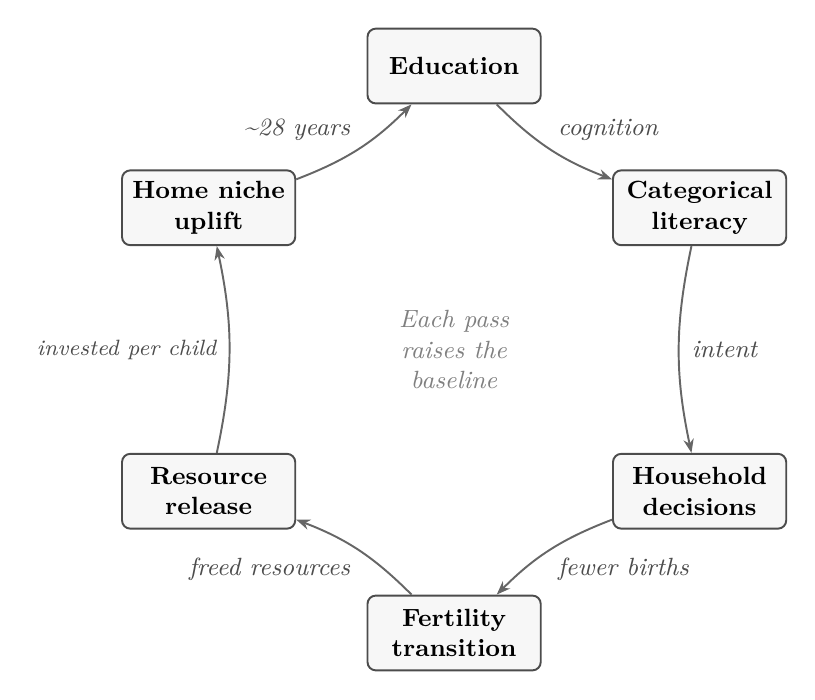
\begin{tikzpicture}[
  box/.style={rectangle, rounded corners=3pt, draw=black!70, fill=black!3,
              line width=0.7pt, minimum width=2.2cm, minimum height=0.95cm,
              font=\small\bfseries, align=center},
  elabel/.style={font=\small\itshape, text=black!70},
  >=Stealth,
  every path/.style={line width=0.7pt, draw=black!60}
]

% ── Loop nodes (hexagonal layout) ──
\node[box] (edu)  at (90:3.6)   {Education};
\node[box] (cat)  at (30:3.6)   {Categorical\\literacy};
\node[box] (hh)   at (-30:3.6)  {Household\\decisions};
\node[box] (fert) at (-90:3.6)  {Fertility\\transition};
\node[box] (res)  at (-150:3.6) {Resource\\release};
\node[box] (pt)   at (150:3.6)  {Home niche\\uplift};

% ── Loop arrows (clockwise, slight bend) ──
\draw[-{Stealth[length=5pt]}] (edu)  to[bend right=12] node[elabel, above right=-1pt] {cognition}    (cat);
\draw[-{Stealth[length=5pt]}] (cat)  to[bend right=12] node[elabel, right=1pt]        {intent}       (hh);
\draw[-{Stealth[length=5pt]}] (hh)   to[bend right=12] node[elabel, below right=-1pt] {fewer births} (fert);
\draw[-{Stealth[length=5pt]}] (fert) to[bend right=12] node[elabel, below left=-1pt]  {freed resources}  (res);
\draw[-{Stealth[length=5pt]}] (res)  to[bend right=12] node[elabel, left=1pt]         {\footnotesize invested per child} (pt);
\draw[-{Stealth[length=5pt]}] (pt)   to[bend right=12] node[elabel, above left=-1pt]  {\textasciitilde 28 years}         (edu);

% ── Centre annotation ──
\node[font=\small\itshape, text=black!50, align=center] at (0,0) {Each pass\\raises the\\baseline};
\end{tikzpicture}
\caption[The generational transmission loop]{The generational transmission loop. Absorption from the school niche installs categorical literacy in the individual brain; at population scale, the same absorption sustains literate CT as the society's transmission regime. Categorical literacy shapes household decisions; household decisions drive the fertility transition; fewer children per household releases resources; those resources raise the literacy of the next generation's home niche, lifting absorption of the school niche. Each pass through the \textasciitilde{}28-year cycle clicks the ratchet one notch.}
\label{fig:loop}
\end{figure}

\subsection{From Action to Talk: How Education Reaches Beyond the Household}\label{from-action-to-talk-how-education-reaches-beyond-the-household}

Education's effects start in the household but do not stay there. The
four radii shown in Figure~\ref{fig:radii} extend education's effects
outward from the Household decisions node of the generational loop
(Figure~\ref{fig:loop}), with decreasing durability as the radius
widens.

\begin{figure}[htbp]
\centering
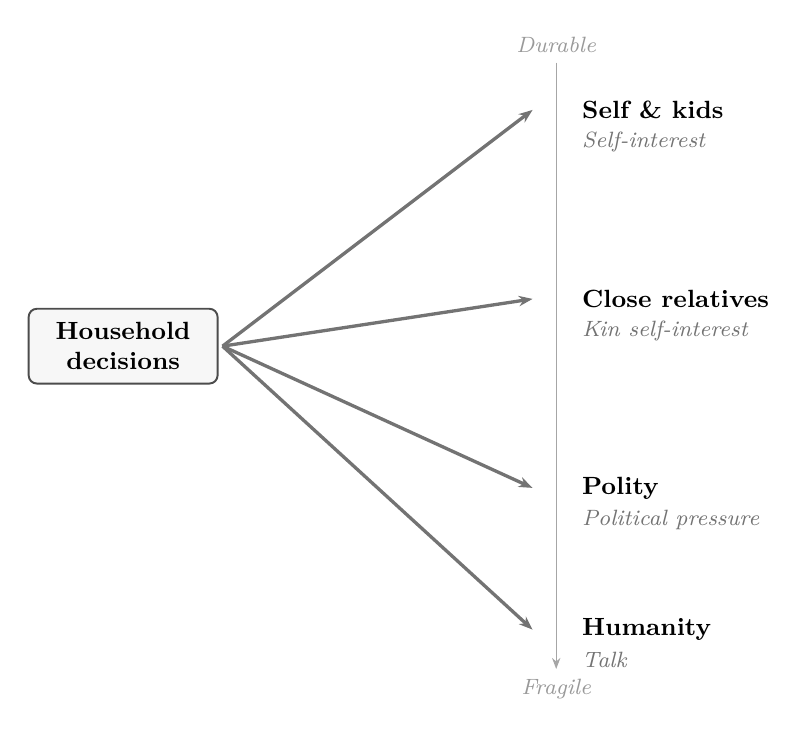
\begin{tikzpicture}[
  box/.style={rectangle, rounded corners=3pt, draw=black!70, fill=black!3,
              line width=0.7pt, minimum width=2.4cm, minimum height=0.95cm,
              font=\small\bfseries, align=center},
  >=Stealth,
  every path/.style={line width=0.7pt, draw=black!60}
]

% ── Anchor node on the left ──
\node[box] (hh) at (0,0) {Household\\decisions};
\coordinate (origin) at ($(hh.east)+(0.05,0)$);

% ── Four radii ──
\draw[-{Stealth[length=5pt]}, line width=1.2pt, black!55]
  (origin) -- (5.2, 3.0);
\draw[-{Stealth[length=5pt]}, line width=1.2pt, black!55]
  (origin) -- (5.2, 0.6);
\draw[-{Stealth[length=5pt]}, line width=1.2pt, black!55]
  (origin) -- (5.2, -1.8);
\draw[-{Stealth[length=5pt]}, line width=1.2pt, black!55]
  (origin) -- (5.2, -3.6);

% ── Durable/Fragile axis ──
\draw[-{Stealth[length=4pt]}, black!35, line width=0.5pt] (5.5, 3.6) -- (5.5, -4.1);
\node[font=\footnotesize\itshape, text=black!40, anchor=south] at (5.5, 3.6) {Durable};
\node[font=\footnotesize\itshape, text=black!40, anchor=north] at (5.5, -4.1) {Fragile};

\node[anchor=west, font=\small\bfseries, text=black] at (5.7, 3.0) {Self \& kids};
\node[anchor=north west, font=\footnotesize\itshape, text=black!55] at (5.7, 2.85) {Self-interest};

\node[anchor=west, font=\small\bfseries, text=black] at (5.7, 0.6) {Close relatives};
\node[anchor=north west, font=\footnotesize\itshape, text=black!55] at (5.7, 0.45) {Kin self-interest};

\node[anchor=west, font=\small\bfseries, text=black] at (5.7, -1.8) {Polity};
\node[anchor=north west, font=\footnotesize\itshape, text=black!55] at (5.7, -1.95) {Political pressure};

\node[anchor=west, font=\small\bfseries, text=black] at (5.7, -3.6) {Humanity};
\node[anchor=north west, font=\footnotesize\itshape, text=black!55] at (5.7, -3.75) {Talk};

\end{tikzpicture}
\caption[Four radii of educational effect]{Four radii of educational effect --- each a boundary draw
of the same coalitional in-group mechanism, with durability
decreasing as the boundary widens: action at the kin scale,
political pressure at the polity scale, talk at the humanity scale.}
\label{fig:radii}
\end{figure}

The home niche operates through action --- the household decisions of
educated adults. But education's effects extend beyond the household,
and the nature of that extension changes as the radius widens. Two
things widen it simultaneously: education expands the boundary of who
counts as ``my people'' --- coalitional psychology (Tooby \& Cosmides
2010) allows flexible group boundaries that education stretches from kin
to polity to humanity --- and it releases surplus, as educated parents have fewer
children and nearly all survive, freeing time, money, and attention.
The arc widens (who you invest in) and the constraint loosens (what you
can invest).

The result is four radii of effect, each a boundary draw of the
same coalitional in-group mechanism, each weaker than the last:

\begin{enumerate}
\item \textbf{Self and children.} Genetic in-group. The home niche
is action: the parents raise the child in front of them, and the
18-year biological channel guarantees delivery. Runs on
self-interest.

\item \textbf{Close relatives.} Kin in-group. Action on siblings,
nieces and nephews, cousins. Runs on self-interest extended by
kinship.

\item \textbf{Polity.} Institutional in-group. Education shifts
citizens' demands on the polity --- voting, organising, professional
norms, policy advocacy. The most likely channel is political
pressure: concrete, but mediated through institutions rather than
direct action. This is where the competing-priority pathway
(Section~\ref{the-generational-transmission-mechanism}) originates.

\item \textbf{Humanity.} Species in-group. Just talk: cross-border
exhortation, conferences, advocacy. No biological or institutional
channel of guaranteed delivery; the outcome depends on whether
someone elsewhere acts on the talk.
\end{enumerate}

The axis that predicts durability is motivational: the home niche
compounds because it runs on self-interest. Every non-education intervention requires
someone to keep serving past the point where self-interest would redirect
them. Revolutionary commitment, donor altruism, state fiscal discipline:
all are fragile because all run against the grain of normal human
motivation. Education runs with it. Non-education intervention buys
time; educational investment changes trajectory.

\subsection{Demographic Structure and the Fertility Transition}\label{demographic-structure-and-the-fertility-transition}

Fertility declines continuously as female education rises,
requiring no threshold to trigger. The
evolutionary mechanism is a shift in reproductive
strategy, not an override of the reproductive drive: in high-mortality
environments, the optimal strategy is quantity --- have many children
because some will die. Education changes both inputs to this calculus.
Child survival rises (fewer births needed to achieve the same number of
surviving children), and the planning horizon extends --- a literate
parent can see that investing more in fewer children produces better
outcomes than hedging with numbers. The drive to maximise offspring
success is unchanged; what changes is the strategy that serves it.

The steepest fertility decline occurs as the cohort crosses into
lower-secondary completion
(Section~\ref{gdp-has-no-independent-effect}). What this depth of
literacy gives the mother is capacity over preferences that already
exist --- the capacity to read a contraceptive instruction, understand
a health protocol, act on a desire not to be pregnant continuously.
This is the mother's own-literacy channel; in the within-country
panel the
active variation sits at lower-secondary depth, because primary is
already approaching ceiling for most of the panel period and the
year-on-year movement in literacy useful for contraceptive action runs
through lower-secondary expansion. On top of it, the grandparent's
literacy adds an independent signal across baselines
(Section~\ref{the-grandparent-channel}) --- never as large as the
parent's own, but never zero --- extending the kin/community radius
back one generation and giving the household additional capacity to
act even where the parent's own schooling is thin. Yet the demographic headwinds are also steepest here:
where total fertility rates are typically above 4, population growth is
rapid, and the gains from each educated cohort are diluted across a
larger and faster-growing next generation. As completion rises, fertility
falls, child survival improves, and household resources per child
increase. The home niche is a household mechanism. States can create
conditions for these decisions; they cannot make them.

The routing is mother-weighted but household-located: both parents act
on household decisions; mothers carry heavier weight on proximate care
because of the biology of pregnancy, nursing, and the daily allocation
of time during the dependency window. Cross-sectional microdata
identifies this within a single country at a single time. At the
country-panel scale, where state-led schooling expansion moves male and
female completion together, the household, not the individual woman, is
the empirical unit (Section~\ref{gdp-has-no-independent-effect}).

Human biology enforces the scale of these decisions. A woman who begins
bearing children at fifteen and has seven will still be pregnant or
nursing at thirty-five --- and the last child, born then, still needs
daily care when she is in her mid-forties. High fertility is not merely
correlated with constrained lives; it is the constraint.

Even in populations where life expectancy at birth is low, women who
survive to childbearing age typically live into their fifties or beyond;
the average is dragged down by infant and child death, not by adults
dying at forty. But survival does not mean freedom. The grandmother
hypothesis in evolutionary biology holds that human females live decades
past menopause precisely because post-reproductive women raised
grandchildren's survival odds. The long post-reproductive lifespan is
itself part of the transmission architecture. Cultural transmission
selected for extended juvenile dependency; extended juvenile
dependency selected for long post-reproductive lives. Together
they are the biological signature of the human developmental niche.

Fertility decline is not a proxy for women's empowerment --- it is the
first expression of it. Education gives capacity over preferences that
already exist: contraceptive availability alone does not produce the
shift; education does. The further dimensions of empowerment that the
literature measures --- labour force participation, household
bargaining power, political voice, economic independence --- follow
after fertility falls, as smaller families free time, resources, and
attention. Education produces the first move; the rest cascades from it.

\subsection{The State: Reach, Not Mechanism}\label{the-state-reach-not-mechanism}

The unit acted upon is the child during the eighteen-year window.
The state is not a substitute for the home niche. It constructs the
second niche --- the school niche --- that, combined with the home
niche, produces the transition state in which children absorb from
both simultaneously. Its reach is the number of children whose
childhoods are loaded by both niches together. Its pace is how
thickly it builds that niche: how many children enrolled, for how
many years, at what quality.

Lutz and Kebede (2018) document the empirical signature of this at
the global scale: state-led educational expansion shifts the
fertility curve down and the life-expectancy curve up at a speed
determined by how quickly the state reaches households whose home
niche still carries the illiterate CT regime. The state matters
because it sets the pace of the ratchet at the population scale; it
does not determine whether, once children have absorbed the school
niche, the adults they become will carry literate CT into the next
generation's home niche. That is guaranteed by the biology of the
dependency window.

What follows from that reach the state does not direct. The
convergence is emergent, in the precise sense a starling flock's turn
is emergent: it forms from millions of private household decisions,
each made for its own reasons, with no one coordinating them and
no one --- not the state, not the households --- perceiving the whole
they compose. No household joins a movement; no committee convenes
the fertility transition. The state thickens the school niche and
sets the pace; the pattern that follows is the population's own,
leaderless and unwilled.

This emergence is older than development. Self-organised collective
order is the ancient mode of a social species: the same evolved
sociality that lets a child learn from a non-kin adult
(Section~\ref{cultural-transmission-across-species}) runs the
population's coordination with no coordinator, and it ran the
illiterate world --- high fertility, high mortality --- as leaderlessly,
for millennia, as it runs this one. Biology supplies the emergent form,
common to both regimes; literate CT supplies only the direction ---
which equilibrium the flock turns toward. The convergence is what an
evolved social species does once the regime flips, not an anomaly
needing its own cause.

The pattern is unwilled, but the decisions it
is built from need not be; Section~\ref{the-decision} is the case for
making them deliberately.

The operative question, in any country that has not crossed the
development threshold, is not whether the state will invest in
education --- all states claim to --- but whether it invests with
\emph{singular priority}. Three regimes recur:

\begin{itemize}
\item \textbf{No priority.} The state does not build schools, does
not train teachers, does not ensure access. Only the home niche
exists, and it gates forward whatever CT regime it inherited.
Pre-industrial populations lived in this regime for millennia.

\item \textbf{Competing priority.} The state builds schools and
trains teachers, but education competes with health, nutrition,
security, governance, and other demands for budget and political
attention. The school niche exists but is thin: modest enrollment,
few years, variable quality. Absorption per child is limited, the
ratchet clicks one notch per generation, and the development
threshold is crossed at a multi-generational pace.
Chapter~\ref{country-histories} traces this through Sri Lanka's earlier
phases, India, and much of sub-Saharan Africa.

\item \textbf{Singular priority.} The state makes education the
unconditional focus and builds the school niche ahead of need ---
schools before children exist to fill them, teachers before
students exist to teach, standardisation before local pressure
demands it. Absorption per child is high because the school niche
is thick. The ratchet clicks several notches per generation, and
the development threshold is crossed within one. Knox's Scotland,
Meiji Japan, post-war Korea, Taiwan, and revolutionary Cuba all ran
this regime.
\end{itemize}

The household operates within whichever school niche the state
provides. Bangladesh from the 1990s illustrates the
home-niche/school-niche interaction. The state-led push for girls'
secondary education reached households whose home niche carried
illiterate CT. The girls who absorbed the school niche then
carried literate CT into the next generation's home niche, making
the household decisions --- fertility, health, investment --- that
produced the next generation's gains (Bora et al.~2022;
Section~\ref{four-further-cases}). Mullainathan and Shafir (2013) describe
the bandwidth tax of the illiterate home niche: evaluating delayed,
abstract returns requires the cognitive reorganisation that only
absorption from a literate niche produces. The state's reach
constructs the school niche; the home niche, once uplifted by a
first-generation school-niche absorber, compounds the gain across
generations.

\subsection{Why Education Is the Limiting Factor}\label{education-as-limiting-factor}

Childhood plasticity is bounded. The dependency window
(Section~\ref{the-dependency-window}) loads the cognitive substrate
across roughly eighteen years; once it closes, schooling reached
is schooling kept. Adult re-entry into formal schooling exists ---
literacy classes, mid-life degree completion, returning students
--- but at frequencies far below what would shift a country's
educational stock at population scale. The exceptions remain
exceptions.

By age twenty-five, education is fixed for life for a given cohort.
The country's adult educational distribution at any time is the sum
of cohort distributions already past that age. It can be added to
only by demographic turnover --- births of new children, ageing of
existing cohorts, deaths of older ones --- the process Lutz (2013)
names \emph{demographic metabolism}. Education stock changes at
the speed of that metabolism: a country shifts its adult
educational mix only as fast as new, more-schooled cohorts displace
older, less-schooled ones in the population.

This is not symmetric with other policy levers. Institutions can be
reformed in years; commercial regulation can be liberalised in a
parliamentary session; tax codes, property regimes, and trade rules
can be changed before lunch. The educational endowment of the adult
population cannot. It is the slowest-moving variable in the policy
ledger and, for that reason, the binding one. The ceiling on a
country's developmental trajectory is set by the educational stock
it has --- not by the institutions, the markets, or the rules layer
that change underneath an unchanged input.

This is why development under competing priority feels slow to
those who want it. The mix of educated and uneducated adults is
what it is at any moment, and the metabolism that would refresh
that mix runs at biological speed. Reformers reach for the levers
they can move --- legal codes, fiscal policy, market regulation
--- and find that the underlying trajectory does not change,
because the input the levers act upon is unchanged. The asymmetry
is also why education is sufficient as well as necessary: an
educated population can change institutions, rewrite rules, and
adopt new technologies at policy speed; an uneducated population
cannot, no matter how good the rules layer is.

Education (Section~\ref{the-decision}) is the only intervention
that alters the metabolism's input; singular priority is its
maximum-speed setting. A government that
gets the rules wrong can fix them next year. A government that gets
the schooling decision wrong loses a generation. The institutional
rebuttal in Section~\ref{the-institutional-challenge} is a
consequence of this argument, not an additional one.

This is also why no other variable has, or can have, education's
influence. The juvenile dependency window
(\S\ref{the-dependency-window}) is the only window in which the
cognitive substrate is loadable, and education is the only
intervention that loads it. Institutions, markets, technology,
capability provision --- every other lever the discipline names ---
act on adults already formed, on a substrate already set. They can
be applied, refused, optimised, or wrecked; they cannot remake the
input. The asymmetry is not a measured effect that further evidence
might overturn. It is the structure of the species. A variable that
acts on the substrate during the window is in a different category
from a variable that acts on the output once the window is closed;
that is the category education occupies alone.

The asymmetry runs inside education as well. The distance from no
formal education to any formal education is categorical: it is the
difference between a brain that has been reorganised by the
dependency window's loading and one that has not. The distance from
a bad school to a great school is marginal by comparison. The
curriculum wars argue over the second contrast and leave the first
contrast unmade.

The panel's measurement convention reflects the same logic. The
20--24 cohort age captures education at the point the schooling
decision has resolved for that cohort: schooling is substantially
complete, upper-secondary either achieved or not, and adult re-entry
rare enough that it does not materially shift the distribution
(Section~\ref{why-lower-secondary-completion}). The country's permanent
educational stock for that generation is what the 20--24 cohort
distribution shows.

\subsection{Why I Measure at Lower Secondary Completion}\label{why-lower-secondary-completion}

I measure development at lower secondary completion --- nine years
of schooling, finished at roughly age fifteen --- because that is
the point inside the long childhood at which enough has been loaded
for the resulting cohort to start acting through it. Three
independent considerations converge on that floor. The
argument is biological first; data availability follows.

First, the regime floor. By roughly fifteen, the biological,
reproductive, and cognitive thresholds of
Section~\ref{the-threshold-of-agency-transfer} are substantially in
place. The cultural-transmission regime is by then enough to be
acting through household decisions --- fertility, child survival,
the home niche the next generation inherits. Lower-secondary
completion is the operational marker: the point at which reading for
unfamiliar content, engagement with formal institutions, and
numeracy beyond counting become normal household activity rather
than skills the household has but does not use.

Second, the empirical floor. Lower-secondary is the level below which
full convergence on all three outcomes (TFR, LE, U5MR) does not
complete, with further completion compounding the signal continuously
beyond it (Lutz \& Kebede 2018). TFR crosses at lower lower-secondary
completion than LE; the threshold-crossing record and the reason are
in \S\ref{literate-ct}.

Third, the data is available where the threshold is. WCDE v3
supplies long-run lower-secondary completion estimates back to 1875
across the panel; higher-secondary and tertiary series cover
narrower windows and fewer countries. The measurement convenience
matches the threshold --- fortunate, not foundational.

The nine-year floor is not a ceiling on what biology supports.
Singapore, Taiwan, Korea, and the Nordic countries run the dose to
the end of the dependency window
(Section~\ref{the-window-supports-a-continuous-dose}); where the
option is given, most of the cohort continues. The window is
eighteen years; fifteen is the floor for when enough of the next
generation's regime is in place to act.

\section{The Prediction}\label{the-prediction}

The claim this chapter tests is that education is the necessary and
sufficient population-scale input for convergence.

A causal model, if real, entails empirical patterns that the data
must show (Pearl 2009). These predictions follow from the biology
set out in Chapters~\ref{longest-juvenile-dependency}--\ref{generational-transmission-and-state},
not from the data; they are deduced from the mechanism, not fitted
to outcomes. Chapter~\ref{the-panel} is the formal check. If the
mechanism is real --- if extended juvenile dependency creates a
biological channel for cultural transmission, and formal education
is the most powerful payload ever delivered through that channel ---
then six empirical patterns must hold. The outcomes across which
those patterns must appear --- fertility, longevity, offspring
survival --- are the classical fitness components of life-history
theory (Stearns 1992).

\begin{enumerate}
\item \textbf{Generational timing.} Because the home niche is
loaded through the juvenile dependency window (Level 1), which
closes around age 18 (Section~\ref{the-dependency-window}), and
educated children reach household agency --- first marriage,
first pregnancy, first independent health decision --- in the
early-to-mid twenties, education at time $T$ should register in
development outcomes at $T+{\sim}28$ (the biological generation
cycle, $\overline{\mathrm{MAC}} = 28.8$ years across the
expansion-phase panel, Section~\ref{the-generational-lag}) --- and,
where the 20--24 cohort at $T$ is already inside its own
reproductive and productive window, at shorter lags as well: log GDP
registers contemporaneously (lag~0, the educated worker's current
output), TFR at $T{+}5$ (the reproductive peak), and under-5
mortality at the childrearing window (lag 10--15). Life expectancy
at birth registers at that same childrearing window (lag~12): it is
mechanically dominated by child mortality, so the schooling that
moves it is the same schooling that moves under-five mortality, not a
separate adult-longevity clock a generation back. The lag signatures
are biological and outcome-specific; the independent grandparental
channel is separable only for TFR and U5MR
(Section~\ref{the-generational-lag}).\label{pred:timing}

\item \textbf{Multi-generational persistence.} Because home-niche
loading (Level 1) routes through the dependency window in every
generation
(Chapter~\ref{generational-transmission-and-state}), a parent's
educational depth installs cognition that the child installs in turn,
so education's predictive power should decay slowly across
generational depths (56, 84, 112 years). Income, which has no
transmission channel equivalent in bandwidth or duration to the
dependency window, should collapse within one
generation.\label{pred:persistence}

\item \textbf{Asymmetric disruption.} Because the payload lives in
the educated adult (Level 1), not in the institutions, income, or
infrastructure that delivered the schooling (Level 2)
(Sections~\ref{the-generational-transmission-mechanism}
and~\ref{the-state-reach-not-mechanism}), destroying the educated
population should reset generational progress, while destroying the
Level-2 shell while leaving the educated population intact should
not.\label{pred:disruption}

\item \textbf{GDP independence.} Because GDP is the
national-accounts face of the Level-2 (literate-CT) regime ---
services and the industrial conversion of materials done by educated
populations --- income carries no separate channel to development
outcomes. Once education's signal is stripped from GDP, what remains
should have no independent predictive power
(Section~\ref{gdp-has-no-independent-effect}).\label{pred:income}

\item \textbf{Universality.} Because both Level 1 (home-niche
loading through extended juvenile dependency) and Level 2
(cumulative cultural transmission through population-scale
schooling) are species-level capacities
(Chapters~\ref{longest-juvenile-dependency}--\ref{cultural-transmission}),
not institutional products, the pattern should hold across political
systems, cultures, geographies, and colonial
histories.\label{pred:universality}

\item \textbf{Collective action.} Household cognitive capacity
(Level 1) aggregates into societal coordination capacity (Level 2):
the same parents who plan family size and seek timely care also
substitute foods under shortage, coordinate migration, pressure
authorities for relief, sustain compliance with public-health
regimes, and run the institutions that respond to shocks --- the
Level-2 categorical claim (Section~\ref{literate-ct}). Societies
that do these things are societies whose households can. The capacity is one mechanism with many testable forms. The strongest
test is famines averted under severe food shocks
(Section~\ref{the-famine-test}). Adjacent forms: the fertility and
mortality transitions running together, the routine functioning of
democratic accountability where mass education has arrived, the
defensive capacity that has kept educated populations from being
colonised in the modern record. Where demographic pressure is also
present, the same capacity projects organised force outward
(Chapter~\ref{the-dark-parallel}). The capacity to avert
famine is not a separate faculty from the capacity to run the
demographic transitions or to defend against external projection
(Section~\ref{the-generational-transmission-mechanism},
Chapter~\ref{why-the-loading-in-childhood-is-invisible}) --- it is the same capacity
at scale.

Educated populations should display this capacity across its
range; uneducated populations facing equivalent pressures should not.
Where the asymmetry runs in the modern direction --- educated
populations no longer under demographic pressure, populations still
mid-transition under continued pressure --- the pressure cannot
translate into projection against the educated population, because the
projecting capacity is what is missing
(Chapter~\ref{convergence-and-peace}). Exceptions to the prediction
should require external force physically suppressing the educated
population's capacity to act.\label{pred:collective-action}
\end{enumerate}

Chapter~\ref{natural-experiments} tests them in natural experiments where the design is cleaner than the cross-country regression can deliver; Chapter~\ref{the-panel} then shows the population-scale signatures in the 185-country panel.

\subsection{Necessity and sufficiency, stated forward}\label{necessity-sufficiency-forward}

\textbf{Necessity, stated forward.} I claim that lower-secondary completion is necessary for the joint crossing of TFR$<$3.65 and LE$>$69.8. In the panel of seventy-three non-oil joint crossers with available data, I find no country that crossed with lower-secondary completion in the 20--24 cohort below 36\% at the year of crossing --- 35\% rounded, the necessity floor. I therefore predict that none of the thirty-one non-converged countries will jointly cross both demographic thresholds with lower-secondary completion below 35\%. Single-threshold crossings --- LE-only via oil rents, TFR-only via local shocks --- are not counterexamples; the claim is about the joint crossing. A country that lands both thresholds below 35\% breaks my necessity claim.

\textbf{Sufficiency, stated forward.} I claim that lower-secondary completion is sufficient for the joint crossing when the 20--24 cohort expands at 1.25 percentage points per year or more from below 10\% and the channel runs undisrupted. Among the rate-subset countries that meet these conditions in the historical panel, lags from passing the 35\% floor to joint crossing run from sixteen years (Cuba, 1958$\to$1974) to thirty-three years (Indonesia, 1984$\to$2017), with South Korea at thirty (1957$\to$1987) and China at twenty-six (1968$\to$1994). I therefore predict that any future country meeting both conditions will cross both demographic thresholds within thirty years of passing the 35\% floor --- thirty is my forward bet, tighter than Indonesia's historical thirty-three. A country that meets both conditions and does not cross within thirty years breaks my sufficiency claim. Cases where the channel is disrupted --- by war, occupation, sustained net emigration of the educated, or hollow content --- do not test sufficiency until the disruption ends; they fall under the hollow-education logic of Chapter~\ref{hollow-education}.


\section{The Natural Experiments}\label{natural-experiments}

The panel establishes the patterns. The natural experiments isolate
the mechanism under designs cleaner than cross-country regression can
deliver --- shocks that isolate one variable while holding the others
constant, or within-country cases that eliminate confounders
entirely. Each subsection below tests a prediction stated in
Chapter~\ref{the-prediction}.

\subsection{The Famine Test (Prediction~\ref{pred:collective-action})}\label{the-famine-test}

The famine test is the strongest empirical test of the collective-action prediction (Prediction~\ref{pred:collective-action}). The shock test asks whether education survives crisis. The famine test asks the converse: does education \emph{prevent} the most extreme form of crisis?

Every major famine since 1950 occurred in a low-education setting. Of 21 famines in the dataset, 19 occurred where lower secondary completion was below 50\%. The median education level at the time of famine was 19.6\%; the mean was 25.4\%. The two exceptions --- North Korea (1996, 100\% completion) and Yemen (2018, 68\%) --- both required external force physically preventing food access: totalitarian state control of distribution in the first case, naval blockade in the second. Where the educated population retained agency, famine did not occur.

The near-miss cases make the pattern sharper. Eighteen country-scale near-misses faced shocks comparable to or worse than those that produced famines elsewhere --- Cuba's 35\% GDP collapse when Soviet imports were cut by roughly three-quarters (1993), post-WWII Japan and Germany, Armenia under simultaneous blockade and war (1993), Ukraine under Russian invasion and grain blockade (2022), Kerala under the 1966 monsoon failure --- and none experienced famine. Their median education was 71.6\%, against 19.6\% for famine countries. The near-miss cases span the same decades as the famine dataset (1945--2022), so the comparison is not an era effect.

Educated populations do not starve. They reorganise supply chains, ration collectively, substitute crops, demand state response, and migrate strategically. Uneducated populations, facing the same shock, lack the household-level capacity to adapt and the political capacity to compel response. The mechanism is the home niche operating through the household: the same cognitive and behavioural repertoire that drives the fertility transition also drives famine prevention.

\textbf{Bihar and Kerala, 1966.} The within-country case eliminates every confounder except education. The 1965--66 national drought crashed India's grain production by 19\%. Bihar experienced famine: 70,000--130,000 excess deaths (Dyson \& Maharatna 1992). Kerala --- India's most food-deficit state, 40\% import-dependent, hit so severely that food riots erupted and the UK Parliament identified it as one of the ``most severely hit areas'' --- had no famine. Same Constitution, same free press, same central government, same democratic institutions. Bihar's literacy was 22\% (female: 9\%); Kerala's was 55\% (female: 39\%). (The 1966 figures are literacy rates --- the only education statistic available at state level for that year --- not the lower secondary completion measure used elsewhere in the paper; the gap runs in the same direction under any available measure.)

Sen's claim that ``no famine has ever taken place in a functioning democracy'' (Sen 1999) cannot explain the Bihar--Kerala divergence. Democracy was constant across both states. Education was not. Myhrvold-Hanssen (2003) challenges Sen directly on this point, arguing that Bihar 1966--67 meets any reasonable definition of famine and that the Indian media, ``although free and independent, did not provide reliable information.'' Drèze himself (quoted in Brass 1986) described the evidence that Bihar was a success story as ``precious little.''

What the Bihar--Kerala case isolates is that education is a
community-level shield, not a national one. The state apparatus was
the same across both; the Constitution was the same; the press was
the same. What differed was how many households in each state
collectively made educated decisions about food, migration, and
political pressure. Where most households can and do, the population
forms a shield that national institutions alone do not provide. Where
most households cannot, no national apparatus substitutes for the
missing mechanism. The same pattern extends into the deeper
historical record. The Madras Presidency famines of 1876--78 killed
an estimated five million people (Davis 2001) under the same imperial
administration that was feeding its own educated population at home.
Bengal 1943 and the earlier Irish famines of 1845--49 fit the same
structure. The population that starves is the uneducated one
regardless of which state nominally governs it; the educated
population does not starve, even when its government is the one
presiding over the starvation.

Kerala's own history confirms the mechanism. In 1943, Travancore (pre-independence Kerala) experienced famine under the same structural vulnerability --- extreme food-import dependence --- killing approximately 90,000 people. The difference between 1943 and 1966 was not democracy (Travancore had an elected legislature from 1932) but education: literacy had risen from approximately 30\% to 55\%. The educated population built the institutions --- universal public distribution, food committees, political mobilisation --- that prevented the same structural vulnerability from producing the same outcome.

\textbf{Ireland, 1845--1849.} Ireland is not an exception to the
prediction; it is the deepest historical confirmation, where the
cause of low literacy is itself diagnostic. The Great Irish Famine
killed approximately 1,000,000 people and drove a further 1,500,000
into emigration over the famine decade (Mokyr 1983;
Ó~Gráda 1999). Mortality concentrated in the Irish-speaking Catholic
west and south and was lowest in the Protestant east of Ulster, the
same geographic gradient that ran in pre-famine literacy. The
structural cause was not the potato blight, which struck the entire
island, but the prior colonial suppression of education. The Penal
Laws restricted Catholic schooling for most of 1695--1829; mass
schooling for the Catholic majority began only with the National
School system in 1831, 14 years before the blight, and reached
the famine zones thinnest.

The pre-famine census recorded aggregate
literacy at roughly 47\% for the population aged five and above, but
the distribution was sharply colonial: Protestant Ulster around 65\%,
Catholic Connacht and west Munster around 33\% (Ó~Gráda 1995). Mokyr's
(1983) county-level analysis found literacy a significant negative
predictor of excess mortality while potato acreage did not survive
the same specification, with female literacy carrying the strongest
signal; Ó~Gráda (1999) confirms the gradient. The same Crown, the same
Parliament, the same Poor Law, the same press --- and a population
whose education had been held below the community-shield threshold for
150 years by deliberate state policy. The prediction holds: famine
struck where literacy was lowest. What the Irish case isolates, that
the post-1950 dataset cannot, is the colonial mechanism that produced
the underlying education gradient over 150 years.

\subsection{Cambodia: Destructive Disruption (Prediction~\ref{pred:disruption})}\label{cambodia-the-home-niche-shadow}

Cambodia is the direct test of destructive disruption: what happens
when the educated population itself is destroyed, as opposed to
shocks that damage institutions, income, or infrastructure while
leaving the carriers intact (Section~\ref{the-shock-test}). Together
this subsection and the next test
Prediction~\ref{pred:disruption} as a pair --- destruction of the
carrier resets progress; destruction of everything else does not. Schools are the
delivery mechanism; the educated adult is the loading channel. The
Khmer Rouge destroyed the second and left the first repairable ---
buildings came back within a decade, but rebuilding the channel
required a generation of its own operation. The country experienced
severe disruption under the Khmer Rouge (1975--1979), during which
the education system collapsed. The
data shows two distinct stalls. The first is the exogenous shock itself.
The second --- a generation later --- is the mechanism's prediction: the
home-niche baseline is the binding constraint (Section~\ref{the-generational-transmission-mechanism}).

\begin{center}
\small
\begin{tabular}{@{}ll@{}}
\toprule
1975 & Khmer Rouge takeover; completion 10.1\% \\
1979 & Khmer Rouge falls; educated population destroyed \\
1985 & Completion 9.5\% --- \textbf{first stall} (system collapse) \\
1993 & Paris Accords; UN transitional authority ends \\
1995 & International reconstruction; completion jumps to 35.1\% \\
2010 & Plateau at 31--36\% --- \textbf{second stall} (parental baseline) \\
2011 & Recovery as post-disruption cohort's children enrol \\
\bottomrule
\end{tabular}
\end{center}

\textbf{First stall (1975--1985).} Completion was 10.1\% in 1975, fell to 9.4\% by 1980, and was still 9.5\% in 1985 --- a decade of zero progress.

\textbf{Recovery and second stall (1990--2010).} After the Paris Accords
and UN transitional authority (1991--1993), schools were rebuilt with
sustained international investment. Completion jumped to 35.1\% by 1995
on the back of that reconstruction. Then it stalled again. From 1995 to
2010, completion plateaued at 31--36\%, unmoved despite continued
external funding. The buildings were there; the teachers were there; the
money was there. Progress did not come. The 35\% plateau is what
competing-priority expansion looks like when it interacts with a
parental education shadow: international reconstruction dispersed
resources across health, infrastructure, governance, and education
simultaneously, while the parental cohort remained frozen at
\textasciitilde10\%. Korea proves singular priority can push far beyond
any parental baseline --- but Cambodia after 1991 was not Korea. The
plateau reflects dispersed investment meeting a damaged generational
base.

The first stall is the exogenous shock --- the regime destroyed the
education system. The mechanism predicts the second. It is the
generational shadow:
the children reaching secondary school in 1996--2010 were born
approximately 1982--1996 --- their parents were the cohort whose own
education was frozen at \textasciitilde10\% during 1975--1985 --- the
pre-disruption level, preserved in households even as the school system
collapsed. Countries that started at Cambodia's level in 1960 reached a
median of 21\% by 1985. The children of the frozen cohort inherited a
10\% parental baseline instead of a \textasciitilde21\% one; the plateau
reflects that missing growth. Recovery
from 2011 onward corresponds to the post-disruption cohort's children
finally dominating the school-age population. The regime fell in 1979,
but education remained frozen through 1985 (9.5\%). A generation
(\textasciitilde28 years) from the end of the educational disruption (1985), recovery follows from 2011 --- the generational lag the mechanism predicts (Prediction~\ref{pred:timing}).

Countries that started at Cambodia's level in 1960 reached a median of
46\% by 2015. Cambodia reached 36\%. The buildings came back in 1991;
the mechanism did not recover until 2011. That twenty-year gap is the home-niche shadow.

The shadow is not over. The grandparent channel
(Section~\ref{the-grandparent-channel}) predicts a second, deeper lag.
Children reaching adulthood in 2020--2025 have parents from the
post-reconstruction cohort (35--36\% completion) but grandparents from
the frozen cohort (9--10\%). At low baselines, grandparent education
predicts child outcomes independently of parent education, comparable
in magnitude to but never larger than the parent's own
($\beta_{gp}$\,=\,--0.048 vs $\beta_p$\,=\,--0.068 for fertility).
The Khmer Rouge fell in 1979; the parental shadow lifted in 2011;
the grandparent shadow persists through at least 2035, when the first
post-disruption cohort's children become grandparents themselves.


\subsection{Non-Destructive Shocks (Prediction~\ref{pred:disruption})}\label{the-shock-test}

Where Cambodia tested what happens when the carrier is destroyed,
the shock test asks the converse: what happens when institutions,
income, or infrastructure are shattered while the educated population
itself survives? Exogenous shocks that kill people depress life
expectancy. They do not reverse the fertility transition. The pattern holds across every shock type in the dataset.

\refstepcounter{table}\label{tab:shock}\addcontentsline{lot}{table}{\protect\numberline{\thetable}Exogenous shocks and development outcomes}Table~\thetable: Exogenous shocks and development outcomes.

{\small
\begin{longtable}[]{@{}
  >{\raggedright\arraybackslash}p{(\columnwidth - 8\tabcolsep) * \real{0.2000}}
  >{\raggedright\arraybackslash}p{(\columnwidth - 8\tabcolsep) * \real{0.1800}}
  >{\raggedright\arraybackslash}p{(\columnwidth - 8\tabcolsep) * \real{0.2200}}
  >{\raggedright\arraybackslash}p{(\columnwidth - 8\tabcolsep) * \real{0.2200}}
  >{\raggedright\arraybackslash}p{(\columnwidth - 8\tabcolsep) * \real{0.1800}}@{}}
\toprule
Shock type & Country & LE effect & TFR effect & Edu effect \\
\midrule
\endhead
Civil war & Sri Lanka & Delayed 12 yr & On path & None \\
State collapse & Russia & $-$5 yr (back) & On path & None \\
Pandemic (HIV) & South Africa & $-$9 yr (back) & On path & None \\
Income destruction & AFC (5 countries) & None & On path & Continued rising \\
Population destruction & Cambodia & Stalled & Lags & \textbf{Reset} \\
\bottomrule
\end{longtable}\addtocounter{table}{-1}% undo longtable's auto-step (we use manual \refstepcounter for labels)
}

\begin{minipage}{\dimexpr\textwidth-2em}
\scriptsize
\textbf{Notes:} LE effect: deviation from pre-shock trajectory. TFR
effect: deviation from education-predicted path. Sources: World Bank
WDI, WCDE v3. Sri Lanka in Section~\ref{four-further-cases}; Cambodia in
Section~\ref{cambodia-the-home-niche-shadow}.
\end{minipage}

TFR is a household decision running on the home niche --- internal to
the household, unreachable by war, virus, or collapsing state. LE depends partly on
whether external conditions allow survival. When the two diverge --- TFR
continuing its education-predicted decline while LE collapses --- the
divergence identifies the shock as external rather than educational.

\textbf{Russia} (99\% lower secondary completion, 1990). The Soviet
dissolution crashed life expectancy from 69.5 to 64.5 (1988--1994) ---
5 years lost in six. TFR, already at 1.89, continued below replacement
throughout --- 1.20 by 2000, never reversing. The state dissolved; the
educated population did not. LE returned to its pre-collapse level by
2009 (68.7) and reached 73.1 by 2019 --- surpassing the Soviet-era peak
by 3.6 years. Education predicts the recovery trajectory, not immunity
to state collapse.

\textbf{South Africa and the HIV epidemic.} South Africa tests
Prediction~\ref{pred:disruption} under a health shock whose biology
is exogenous to education. Between 1990 and 2005 LE fell from 62.9
to 53.9 (the largest peacetime LE reversal in modern history) while
TFR fell from 3.72 to 2.51 and lower-secondary completion rose from
64.5\% to 82.6\%. TFR registers contemporaneously to the mother's
own depth and tracked the lower-secondary expansion on schedule.
LE's behavioural response to a novel pathogen requires schooling
depth at acquisition age, set in the prior generation's window ---
the cohort entering reproductive age 1990--2005 grew up under
apartheid education too shallow to deliver it. Post-ARV, LE recovered
to 66.1 by 2019. The full mechanism --- apartheid stratification of the
1990 aggregate --- is in Section~\ref{south-africa-case}.

Cambodia (Section~\ref{cambodia-the-home-niche-shadow}) is the exception that
proves the rule: the only shock that breaks the household mechanism is
the one that destroys the household.

\subsection{The Colonial Test (Prediction~\ref{pred:universality})}\label{the-colonial-test}

The famous settler mortality instrument does not measure institutions. It measures whether Protestant colonisers --- who built schools --- survived.

Acemoglu, Johnson \& Robinson (2001) use settler mortality as an
instrument for institutional quality: where European settlers survived,
they built inclusive institutions; where they did not, they built
extractive ones. The instrument cannot distinguish this from an
alternative channel: where \emph{Protestant} settlers survived, they
built \emph{schools}. The Reformation made mass literacy a theological
obligation (Section~\ref{the-generational-transmission-mechanism}). The Counter-Reformation removed it. Protestant
colonisers (Britain, the Netherlands) transplanted mass education
systems. Catholic colonisers (Spain, Portugal, France, Belgium) did not.
AJR's instrument captures this difference and attributes it to
institutions.

The data separates the two channels. On AJR's 64-country base sample,
education at independence (1950 lower secondary completion) explains
52\% of the variance in current log GDP per capita; AJR's own
institutional measure (\emph{avexpr}, average expropriation risk
1985--95) explains 53\%. The two are highly collinear ($r = 0.62$):
settler mortality predicts both, because where Protestant settlers
survived they built the schools, and the schools made the inclusive
institutions possible. The
collinearity is the structural finding --- the IV identification AJR
claim cannot decompose the two channels because the same colonial-era
variation drives both. Coloniser religion alone explains 6\% of GDP
variance, but adding religion to a model that already contains
education raises R$^2$ from 0.518 to 0.521. Religion predicts GDP only
because it predicts education. Once education is in the model,
religion adds nothing. The channel is religion $\to$ schools $\to$
education $\to$ development.

The 2SLS first-stage diagnostics confirm the structural problem on
AJR's actual variable. Coloniser religion is a strong instrument for
education at independence (first-stage $F=10.71$, above the Stock \&
Yogo threshold) and a borderline one for AJR's avexpr measure
($F=9.61$, just below). The decisive test is the symmetric one:
\emph{avexpr is itself a strong instrument for education}
($F=37.13$, three times the threshold). AJR's own variable, on AJR's
own sample, predicts education with the same first-stage strength
required to call any instrument valid. The exclusion restriction is
empirically violated: settler mortality and avexpr both reach the
outcome through education \emph{and} through institutions, and IV
identification cannot decompose them. Full first-stage and
second-stage coefficients ($\hat\beta=+0.084$, $t=6.74$ when avexpr
instruments education) are in Table~\ref{tab:a6} (full replication in
\texttt{scripts/robustness/iv\_2sls\_colonial\_icrg.py}).

Latin America is the critical case. Spanish and Portuguese colonies were
settler colonial --- Europeans came and stayed in large numbers, built
cities, established legal systems. AJR's framework predicts that
settlement should produce inclusive institutions and therefore
development. It did not. AJR require an ad hoc distinction between
``inclusive'' and ``extractive'' settler colonialism to explain why Latin
America underperforms. The education account needs no such distinction:
Catholic settlers brought no mass education tradition. Spain had 0.6\%
primary completion for its own 1875 birth cohort; Portugal had 0.1\%.
They could not transplant what they did not possess. The educational
base at independence was correspondingly low (mean 11\% lower secondary,
1950), and development followed the education, not the institutions.

The settler mortality instrument is a
Protestant education instrument.

Ireland 1845--49 is the within-polity confirmation
(Section~\ref{the-famine-test}): one Crown, one Parliament, one legal
system --- institutions held constant by being one polity --- with
mortality tracking the literacy gradient the Penal Laws had carved over
150 years. Mokyr's (1983) county-level horse race on the Irish
cross-section already returned the same answer the 64-country sample
returns: literacy is the active variable; institutional proxies are not.

The Protestant channel connects to Easterlin's (1981) original insight:
the divergence in economic growth between early and late industrializers
tracked the divergence in mass schooling --- driven originally by the
Reformation's insistence on personal scripture-reading, which produced
mass literacy across Northern Europe. The distribution of development in
1960 was substantially the distribution of schooling in 1860. Goldin \&
Katz (2008) document the same transmission within the United States: the
``human capital century'' of 1910--1940, driven by the high school
movement, explains the majority of twentieth-century income growth --- a
within-country longitudinal result consistent with the cross-country
generational mechanism estimated here.

\section{The Country Histories}\label{country-histories}

The natural experiments and the country histories are both history. The natural experiments isolate the mechanism inside single shocks; the country histories show it running across full development trajectories --- schools built before factories, literacy before fertility decline, mothers' education before household reorganisation, in observable historical sequence. The panel's forward lag is a coefficient; in the histories, it is a calendar. The history carries the identification; the panel shows the resulting pattern is universal across the species.

Every country that developed did so by loading its children's long childhoods with formal schooling --- fast under singular priority, slower under competing priority, but always through the same eighteen-year window, under every political system, at every income level, on every continent. What is in each country's history is what happened to its children during that window: who built the schools, who reached them, what was loaded into the children, and what the resulting cohort then did as adults.

\refstepcounter{table}\label{tab:transition-year}\addcontentsline{lot}{table}{\protect\numberline{\thetable}Schooling commitment and year of crossing the development threshold}Table~\thetable: The empirical sequence --- each country's schooling commitment and the year it crossed the development threshold.

{\footnotesize
\begin{longtable}[]{@{\hspace{0pt}}l@{\hspace{6pt}}l@{\hspace{6pt}}l@{\hspace{6pt}}l@{\hspace{6pt}}l@{\hspace{6pt}}r@{\hspace{6pt}}l@{\hspace{6pt}}l@{\hspace{0pt}}}
\toprule
Country & Dev. & TFR crossed & LE crossed & Onset & Rate & Lag & Gen. \\
\midrule
\endhead
Taiwan & \textbf{\textasciitilde1970} & \textasciitilde1970 & \textasciitilde1970 & 1950s & 2.15 & \textasciitilde20 yr & \textbf{1} \\
S.\ Korea & \textbf{1987} & 1975 & 1987 & 1953 & 2.13 & \textasciitilde34 yr & \textbf{1} \\
Cuba & \textbf{1974} & 1972 & 1974 & 1961 (40\%) & 2.27 & \textasciitilde13 yr & \textbf{1} \\
Bangladesh & \textbf{2014} & 1995 & 2014 & 1990s & 1.30 & \textasciitilde24 yr & \textbf{1} \\
Sri Lanka & \textbf{1993} & 1981 & 1993 & 1940s--50s & 1.20 & \textasciitilde42 yr & \textbf{2} \\
China & \textbf{1994} & 1975 & 1994 & 1950s+CR & 1.50 & \textasciitilde42 yr & \textbf{2} \\
Kerala† & \textbf{\textasciitilde1982} & \textasciitilde1973 & \textasciitilde1981 & Early 20thC & --- & \textasciitilde65 yr & \textbf{3} \\
India & \textbf{2017} & 1996 & 2017 & 1950s & 0.87 & \textasciitilde67 yr & \textbf{3} \\
Uganda & \textbf{---} & TFR 4.39 & LE 67.7 & None & --- & --- & --- \\
\bottomrule
\end{longtable}\addtocounter{table}{-1}% undo longtable's auto-step (we use manual \refstepcounter for labels)
}

\begin{minipage}{\dimexpr\textwidth-2em}
\scriptsize
\textbf{Notes:} Developed = year both thresholds crossed (TFR
$<3.65$ \emph{and} LE $>69.8$, the 1960 United States values, World
Bank WDI). Expansion onset = year or level at which sustained
educational expansion began. Rate = average annual change in lower
secondary completion from expansion onset to development crossing,
in percentage points per year. Lag = years from onset to development
crossing. Generations = number of $\sim$28-year cycles. CR = Cultural Revolution (1966--76). Cuba's high
starting base (40\%) and the 1961 reconstruction of losses from the
post-revolution exodus shortened the lag below the typical
$\sim$28-year generation. $\dagger$~Kerala figures estimated from
India Sample Registration System and census records; all other
figures from World Bank WDI direct measurement.
\end{minipage}

The earliest modern example is Japan (1872): the Meiji compulsory
education ordinance, implemented through repurposed temples with
community teachers, no substantial budget. The sequence was mandate
before resources --- the state declared compulsory education and built
the infrastructure afterward.

Korea is the calibration case --- the fastest sustained expansion in
the WCDE dataset (Section~\ref{korea-and-philippines}). All other rows in
Table~\ref{tab:transition-year} are independent tests. The expansion rate determines
generations to crossing
(Section~\ref{the-generational-transmission-mechanism}): at Korea's
pace it compresses to one generation; at India's 0.87 pp/yr it spreads
across three.

Three parameters predict crossing time: starting base, expansion rate
relative to the Korea benchmark, and structural disruption. Disruption
delays LE crossing --- Sri Lanka's 12-year TFR-to-LE gap (1981→1993)
maps onto the civil war; China's 19-year gap (1975→1994) reflects
the residual from the 1959--61 famine working through adult cohorts. Korea, Taiwan, Cuba,
and Bangladesh had no comparable disruption. The predicted depths match:
Korea-pace cases in 20--34 years; half-Korea-pace in 42--45 years;
third-Korea-pace in 60--70 years. The crossing dates are the test, not
the inputs.

Read together, the cases hold across regime type (authoritarian,
democratic, socialist, post-colonial, military), ideology (Confucian,
Islamic, Catholic, Buddhist, Marxist-Leninist, Hindu-majority), and
income level --- \$1,038 per capita at Korea's expansion, \$1,159 at
Bangladesh's crossing. This is Prediction~\ref{pred:universality} in
its most direct form. What the cases add beyond the prediction is the
calendar: in each, schooling commitment precedes development by a
generation, observably and in order.

\subsection{Korea and the Philippines (Predictions~\ref{pred:timing} and~\ref{pred:universality})}\label{korea-and-philippines}

In 1950 the Philippines was ahead of Korea on income per capita, and started from a comparable educational base --- 22\% lower-secondary completion against Korea's 25\%. By 2000 Korea had crossed every development threshold; the Philippines had crossed none. The income advantage favoured the Philippines; the educational regime that followed did not. What separated them was what each country chose to load into its children's eighteen years.

Taiwan and Korea are the timing and regime-independence test. Both
were authoritarian during expansion; both crossed one generation after
sustained expansion began. Taiwan and Korea crossed earliest --- both
at benchmark pace, both state-driven from colonial bases built by
Japan (Taiwan 18\%, Korea 25\% completion by 1950). Korea expanded at 2.13 pp/yr, the fastest sustained
rate in the WCDE dataset; Taiwan followed a nearly identical trajectory.
Both had functioning markets --- what Sen calls ``growth-mediated
security'' --- but the growth was mediated by education, not the reverse.
State-driven singular expansion compressed development to 20--34 years
against the 40--70 years seen in competing-priority cases.

American colonial education in the
Philippines built that 22\% base over half a century. In 1960, the Philippines was one of the
most prosperous countries in developing Asia: GDP per capita of \$1,124
against Korea's \$1,038 (constant 2015 USD), ahead of Thailand (\$592),
Indonesia (\$598), and far ahead of India (\$313) and China (\$241). But
no post-independence government sustained the educational investment.
Korea made education the singular priority;
the Philippines drifted at roughly half that pace. The Philippines crossed TFR in 2003 and LE in 2017, then wobbled around the LE threshold through the pandemic; by 2022 it sat at TFR 1.9 and LE 69.5 --- effectively converged, two generations after Korea did so, at roughly half the pace of educational expansion. Education policy is a choice, not an inheritance. Income does not make the choice for you.

Korea also marks the observed maximum, not the ceiling itself. From the 1950 starting position of
twenty-five per cent lower-secondary, biology alone --- nine years from
policy decision to a fully loaded cohort --- would have delivered
universal completion at roughly twice the pace Korea achieved. Even
the WCDE record ran at about half of biological maximum. The ceiling sits well above,
not at, what any country has ever delivered. SDG~4's fifteen-year
window to 2030 for universal upper-secondary (UN 2015) is three
years longer than the biological minimum --- correctly ambitious,
feasible under singular priority. Where the target has been
missed it has been missed under competing priority, not biology.

\subsection{Kerala (Prediction~\ref{pred:universality} at sub-national scale)}\label{kerala}

Kerala tests the mechanism at sub-national scale: the same transition,
the same lag, \textasciitilde35 years ahead of India as a whole
(Kerala \textasciitilde1982; India 2017). Kerala
crossed at \textasciitilde1982 --- the paradigm case of
competing-priority expansion. Education had been building since the
early twentieth century through social reform movements --- gradual
accumulation through social reform and state investment ---
competing-priority, not singular-priority at Korea pace. TFR
crossed by \textasciitilde1973; LE followed \textasciitilde8 years
later. Kerala had extensive state provision --- public health, food
distribution, land reform --- but fertility declined because educated
women made the decision, not because provision was available
(Section~\ref{demographic-structure-and-the-fertility-transition}). The
Emergency sterilisations (1975--77) confirm the polarity: forced on
the least-educated northern states, they brought down the government
(Gwatkin 1979; Vicziany 1982); Kerala needed no coercion. State
coercion either arrives after education has done the work, or fails
where education has not.

The sub-national test has been run systematically. Drèze \& Murthi
(2001), using district-level panel data for 1981 and 1991, found that
women's education was the single most important predictor of fertility
differences across Indian districts, while urbanisation, poverty
reduction, and male literacy showed no significant association. The
cross-country result replicates within a single country at district
level.

Kerala by itself can be read as particular --- its history of social
reform setting it apart. The southern tier makes that reading harder to
sustain. Kerala, Tamil Nadu, Karnataka, and undivided Andhra Pradesh
reached replacement fertility ahead of the northern states often grouped
as BIMARU --- Bihar, Madhya Pradesh, Rajasthan, Uttar Pradesh --- every
southern state crossing before every northern one, the two tiers
separated by roughly a generation; in the most recent survey round Bihar
still stood at 2.76 and Uttar Pradesh only at replacement, while the
south had been below it for decades. The variable that orders the eight
is the level of schooling: female literacy ran 73\% in the south against
55\% in the north, ranking the states almost exactly against their
crossing dates (Spearman's $\rho = -0.85$). I read this as the
within-country form of the finding the panel returns. The southern states
are also, by most measures, better administered, and I do not claim to
separate that from their schooling within this contrast --- the two move
together. What the contrast does hold fixed is the institutions the
account names as primary: one constitution, one supreme court, one
property regime, one central bank, one body of federal law across all
eight states. Where those are common to every state, the development still
sorts by schooling.

\subsection{Four Further Cases}\label{four-further-cases}

Each row below identifies the specific prediction the case most
directly confirms.

\begin{longtable}[]{@{}llp{0.52\textwidth}@{}}
\toprule
Case & Crossed & Prediction tested and result \\
\midrule
\endhead
Sri Lanka & 1993 & \textbf{Prediction~\ref{pred:disruption}} (non-destructive shock). TFR crossed 1981; LE climbed to 69.0 by 1988, fell to 67.3 during the civil war, recovered to 70.0 by 1993. War disrupted the economy and life expectancy without breaking the home niche. \\
Myanmar & --- & \textbf{Prediction~\ref{pred:universality}} (regime independence). 73 years of military rule, GDP \$1,025 (2015), education at 0.6 pp/yr. TFR fell from 5.9 to 2.3; LE rose from 44.1 to 65.3 --- consistent with 43.5\% completion. The regime suppressed speed; it could not reverse what the home niche had already carried forward. \\
Cuba & 1974 & \textbf{Prediction~\ref{pred:universality}} (socialist regime). 40.3\% completion in 1960; post-revolution exodus removed the professional class. The 1961 campaign deployed 268,000 volunteers (Prieto 1981), replacing an elite that left with a mass baseline that stayed. Cuba and Taiwan --- Soviet-aligned and US-allied --- crossed within four years. \\
Bangladesh & 2014 & \textbf{Prediction~\ref{pred:income}} (income independence). 11.4\% completion in 1960, GDP \$1,159 at crossing; Nepal followed in 2022 at \$1,114, even lower. Two crossings below \$1,200 in the dataset. Sustained commitment to girls' education from the 1990s. TFR decline tracks female education expansion, not contraceptive distribution (Bora et al.~2022). \\
\bottomrule
\end{longtable}\addtocounter{table}{-1}% undo longtable's auto-step (we use manual \refstepcounter for labels)

\subsection{China (Prediction~\ref{pred:income} --- the support-led residual is education)}\label{china}

China is the direct test of income-independence against the
support-led-security thesis. Drèze and Sen attributed China's outcome
to direct health provision; the panel shows the residual was
education. China crossed in 1994. Three corrections to the standard
narrative.

First, what is called an educational catastrophe was
the largest educational expansion in Chinese history. The standard
framing conflates the disruption of university education --- a
small percentage of the population --- with the overall
trajectory. For rural China --- 80\% of the population
(National Bureau of Statistics 1982) --- the Cultural Revolution era
produced the largest population-weighted lower-secondary expansion in
the WCDE 1870--2015 record. Cohort-over-cohort gains run +10.6pp for
the birth 1951--55 cohort (in lower-secondary at CR onset), +15.0pp
for birth 1956--60 (peak rural 民办 era), and +10.7pp for birth
1961--65 --- adding roughly thirteen million additional lower-secondary
completers in the 1956--60 birth bracket alone, more than thirty times
South Korea's peak single-cohort gain and over a hundred and fifty
times Cuba's. The cohort that came of school age \emph{after} 民办
collapsed and before the 1986 compulsory-education law (birth
1966--70) shows the smallest gain in modern Chinese history, +2.3pp.
Community schools (民办学校) brought secondary education to
villages that had none (Pepper 1996; Unger 1982; Gao 2008).

Second, China is the most direct test of Drèze and Sen's
support-led-security thesis. Drèze \& Sen (1989, Table~10.6) show
China's under-5 mortality at 32\% of what GNP predicted --- the largest
deviation in their sample --- and attribute it to ``support-led
security'': barefoot doctors (赤脚医生), direct provision. But Sen
regressed on GNP and found a residual. That residual is education.

When life expectancy and under-5 mortality are matched on mean years of
schooling (age 20--24, $\pm$0.5~years of schooling, any calendar year;
the metric used in this section's outcome-matching, distinct from the
lower-secondary completion of the panel chapters --- the two move
together for China across the period) rather than GNP, China's
advantage reverses. China's LE was
\emph{below} education-matched peers from 1965 to 1991 --- 6.6~years
below at 1965, still 2.7 below at 1980, converging only in 1991 --- and
its U5MR was \emph{above} education-matched peers until 2000.\footnote{Mean years of schooling
computed from WCDE~v3 proportions (age 20--24, both sexes); LE and U5MR
from World Bank WDI. Peer pool is all country-years within $\pm$0.5
mean years of schooling of China's value at each year. The result is robust to peer-pool bandwidth: LE and U5MR gaps retain the same signs and comparable magnitudes at $\pm$0.25 and $\pm$1.0 mean years.} The barefoot
doctors were not producing exceptional outcomes; China was
underperforming what its education level predicted.

The barefoot doctors and the community school teachers came from the same
CR-era rural mobilisation (Gao 1999). The doctors were local, culturally embedded,
drawn from the villages they served --- optimally delivered provision.
When Deng dismantled the system after 1980, they left, because rational
people freed from revolutionary ideology redirected their labour toward
self-interest. The LE convergence rate was statistically unchanged:
$+0.31$~years/year before 1981, $+0.30$ after ($\beta_3 = -0.007$, $p =
0.82$). LE continued to rise --- from 64 to 69.8 by 1994 --- because
the educational baseline built into rural households did not leave with
the doctors. Drèze \& Sen (1989, pp.~215--221) document the resulting
health crises and rising rural medical costs (Gao 2008; Liu et
al.~2003), but these crises left no detectable mark on the trajectory.

China crossed to \emph{above} education-predicted LE in 1992 and to
\emph{below} education-predicted U5MR around 2000 --- two decades after
the barefoot doctors were gone. Mean years of schooling rose from 5.9
(1965) to 8.0 (1980) to 9.6 (2000), tracking both outcomes across both
eras.

Third, the TFR threshold was crossed in
1975 --- five years before the one-child policy. China's
fertility trajectory mirrors South Korea and Thailand's, both of
which achieved equivalent TFRs without compulsory policy (Cai 2010;
Babiarz et al.~2018). The policy did not cause the decline; it was imposed on a
transition already in progress, matching peers who reached the same
endpoint without coercion.

\subsection{South Africa: Apartheid Stratification and the PET Curve}\label{south-africa-case}

South Africa's 64\% lower-secondary completion in 1990 is an aggregate
masking apartheid stratification: near-universal white completion and
much lower Black completion produced a bimodal distribution invisible
in national data. That split is not only a measurement artefact; it
is the signature of a boundary drawn by identity --- one line doing
two things at once. It rationed schooling to the white enclave and
withheld it from the Black majority, then held the two apart so the
enclave's development could not cross to the rest. A developed phase
that cannot mix cannot lift its surround, and here the line that
walled it off was the same line that had denied the surround its
schooling. The country begins to cross only as that boundary opens and
the majority's own schooling expands --- which is what the post-1990
expansion traced below records. The population bearing the brunt of HIV had far
lower education than the headline figure suggests. The fall in TFR
from 3.72 (1990) to 2.51 (2005) is the lag-difference between TFR
and LE operating as predicted. Lower-secondary education drives
fertility decline at the contemporaneous lag (panel $R^2 = 0.71$ for
lower-sec~$\to$~TFR at \texttt{LAG\_TFR}), and the post-apartheid expansion of
lower-secondary (64.5\%~$\to$~82.6\% between 1990 and 2005) was
running through the shock --- the current mothers' own depth was
rising fast enough to flip fertility on schedule. The fall is
not a frozen home-niche baseline surviving external disruption ---
1990 would be too early to carry that claim, with TFR still at 3.72,
above the development threshold. It is the ordinary
lower-sec\-ondary-to-fertility mechanism continuing to run while the
prior generation's depth --- the cohort at acquisition age when the
epidemic hit --- remained too shallow in the affected majority to
deliver the behavioural response to a novel pathogen that deeper
schooling, accumulated earlier, carries.

The LE collapse runs through that secondary deficit. The Southern
African epidemic was driven at the acquisition stage by factors
education could not have prevented: low traditional circumcision
prevalence (8--11\% in the HIV belt vs 85--99\% in Muslim West
Africa), which three randomised trials showed provides a 60\%
biological reduction in male acquisition risk (Auvert et al.~2005).
Circular mining migration also created connected sexual networks
across the subcontinent. These are genuinely exogenous to education.

Education was in the story on both sides of the behavioural response.
Early in the epidemic, more educated Africans were \emph{more} likely
to be HIV-positive: greater mobility, more partners, more agency
exercised without information about a novel pathogen (Fortson 2008).
Once information existed, the gradient reversed: educated populations
changed behaviour first. The Botswana 1996 school-reform natural
experiment found each additional year of secondary schooling caused
an 8.1-pp cumulative HIV reduction (De~Neve et al.~2015). The same pattern
appears in rural Uganda, where educated individuals responded more
to prevention campaigns, and the
education--HIV gradient reversed from positive to negative between
1990 and 2000 (De~Walque 2007). Baker et al.\ (2008) formalise this
as the Population Education Transition curve: when a novel health risk
enters a population, the educated are early adopters (positive
gradient); once information exists, the educated change behaviour
first (gradient reverses). The pattern replicates across cigarettes,
processed food, and HIV --- education is the mechanism in both
directions, at the secondary-completion depth the behavioural response
requires.

South Africa's 1990 lower-secondary figure, once stratified, sat
below that depth for the majority who received the shock.

\section{The Panel}\label{the-panel}

\subsection{What the Panel Sharpens}\label{what-the-panel-sharpens}

One lever moves the whole panel. Lower-secondary completion moves
every development outcome --- income, fertility, longevity, child
survival --- each at the lag its own biology sets, and once it is in
the model nothing else adds to it. That is the regularity this chapter
establishes at the scale of the species.

I now turn to society-scale evidence: what the population did from
1950 to 2015, read through within-country fixed effects on the
144-country expansion sub-panel. The biology
(Chapters~\ref{longest-juvenile-dependency}--\ref{generational-transmission-and-state}),
the country histories
(Chapters~\ref{natural-experiments}--\ref{country-histories}), and the
falsification (Chapter~\ref{hollow-education}) identify the channel;
the panel sharpens it at the scale of the whole species. It does what
the case work cannot: show that education, fertility, longevity, and
child survival moved together across the full universe of countries;
that log GDP per capita, stripped of education's contribution, predicts
none of the development outcomes; that the pattern holds in every
region, era, and income band; and that none of it depends on the
estimator, from regularised linear regressions to a country-blind
transformer (Section~\ref{every-method-agrees}). The objection that the
mortality decline is exogenous medical technology is answered
separately (Section~\ref{the-deaton-objection}).

\subsection{The Specification}\label{the-specification}

Every panel result in this chapter comes from one estimating equation.
For country $i$, a development outcome $Y$, and a lag $L$ set by the
biology of the channel,
\[
Y_{i,\,t+L} \;=\; \alpha_i \;+\; \beta\,E_{i,t} \;+\; \varepsilon_{i,t},
\]
where $E_{i,t}$ is lower-secondary completion (both sexes, age 20--24)
in year $t$, $\alpha_i$ is a country fixed effect, and $L$ is the
outcome's biological horizon --- $0$ for GDP, $5$ for fertility, $12$
for life expectancy and under-five mortality, and $28$ for the
child-education step where the outcome $Y$ is the next cohort's own
completion (Section~\ref{the-generational-lag}). Outcomes enter in logs
where the table so notes. I estimate $\beta$ within countries and
cluster the standard errors by country.

Three design choices carry the specification, each argued where it does
its work. I read $\beta$ only within countries --- the fixed effect
$\alpha_i$ absorbs everything time-invariant (geography, founding
institutions, culture, colonial inheritance), so it comes from a
country's own schooling and its own later outcomes, never from
comparisons between countries. I lag every outcome forward of the
schooling that predicts it, so the cause precedes the outcome and the
forward structure closes the reverse reading
(Section~\ref{the-generational-lag}). And I do not control for GDP,
because income sits on the causal path --- schooling builds the
population that produces it --- so holding it fixed would block the
pathway and fold education's effect into a downstream proxy
(Section~\ref{gdp-has-no-independent-effect}). None of this is
knife-edge: each outcome's signal rises and falls gradually around its
window, so the finding is a property of the mechanism, not the exact
year read.

This is the whole apparatus the argument needs on the page. The
headline robustness --- that no estimator, from regularised linear
models to a country-blind transformer, moves the answer --- is in
Section~\ref{every-method-agrees}. The full battery (Frisch-Waugh-Lovell,
unique-$R^2$ decompositions, the 20-test diagnostic suite, robustness
sweeps, and the marginal-effect machinery) is in \texttt{scripts/},
indexed by \texttt{scripts/ECONOMETRICS.md}.

\subsection{The Generational Lag}\label{the-generational-lag}

The same regression $\text{edu}(T) \to \text{outcome}(T{+}L)$ measures
different mechanisms at different lags $L$. The panel uses four
timescales, anchored on the biological generation cycle.

\paragraph{Four time constants, not to be conflated.} The argument
carries four distinct intervals, and collapsing any two of them
misreads the panel. (i)~The \emph{juvenile dependency window}, roughly
eighteen years, is the span over which the child is loaded; agency
transfers inside it, around fifteen
(Section~\ref{the-threshold-of-agency-transfer}). (ii)~The
\emph{measurement age} is the 20--24 cohort, where completion is read
once schooling has resolved; its midpoint, about twenty-two, is the
origin the forward lags are counted from --- not the age of agency, and
not birth. (iii)~The \emph{per-outcome biological lag} is the distance
from that measurement to when each outcome registers: zero for income,
five for fertility, twelve for life expectancy and child survival.
(iv)~The \emph{generational cycle} is the parent-cohort-to-child-cohort
step --- the education-to-education lag and the headline $T{-}28$, with
empirical cohort interval $\overline{\mathrm{MAC}} = 28.8$ years. The
lags in (iii) are short because the measured cohort is already inside
its own reproductive and working window; the cycle in (iv) is long
because it waits for that cohort's children to reach the same age.
Different clocks, one biology.

Because childbearing, childrearing, and the working life each spread
across a range of ages rather than concentrate on a single year, and
education's effect on every outcome is continuous, the lag profile is
smooth: each outcome's signal rises and falls gradually around its
mechanism's window, with no knife-edge at any particular year. The
specific lag I read an outcome at, within its biologically plausible
window, is therefore not load-bearing --- the result is a property of
the mechanism, not an artifact of lag selection, and the lag-sweeps in
this section and the next confirm it. I report each outcome at the
center of its window for interpretability, not because the finding
turns on the choice.

\paragraph{The biological generation cycle ($\sim$29 years).} The
cohort-weighted mean age at childbearing pooled across the
expansion-phase panel (UN WPP 2024, $n=1{,}609$ country-years, $177$
countries) is $\overline{\mathrm{MAC}} = 28.8$ years. The interval
moves only $\sim$1.0 year across lower-secondary completion bins
($29.3$ at low education, $28.2$ at high) --- educated women delay
first birth but bear fewer children, and the mean barely moves. This
invariance is what makes one generational step a well-defined unit
at population scale. The 28-year cross-generation step --- the lag for
edu-to-edu transmission and the joint forward-prediction headline --- is a
slight underestimate of the empirical cycle; the lag-sweep profile
(Section~\ref{the-shape-of-the-response})
is smooth enough that the existing $T{+}28$ results carry through.

\begin{center}
\footnotesize
\begin{tabular}{@{}p{3.4cm}p{4.2cm}p{6.7cm}@{}}
\toprule
Timescale & What it measures & Mechanism \\
\midrule
Contemporaneous (lag 0 for GDP; lag 5 for TFR) &
The 20--24 cohort's education and its near-term outcome ---
log GDP at the same year; TFR at $T{+}5$, when the cohort
reaches its reproductive peak. &
The cohort is already in its reproductive and productive window;
literacy acts in real time. Mothers read contraceptive instructions
and act on them; educated workers contribute to current GDP. \\
\addlinespace
Childrearing window (lag 10--15; U5MR and LE) &
The 20--24 cohort's education and both under-five mortality and
population life expectancy 10--15 years later. &
The cohort's own children must be born and survive to age 5 before
the survival outcome registers. Life expectancy at birth is
mechanically dominated by child mortality, so it moves with the same
childrearing-window schooling rather than on a separate adult-longevity
clock a generation back. \\
\addlinespace
Cross-generation step ($\sim$25--30 years) &
The 20--24 cohort at $T$ and outcomes observed at $T{+}28$: their
daughters' education stock, the next generation's TFR via their
daughters' decisions, and the next generation's U5MR via the
system-level health environment the now-grandparental generation
built. &
One full generational step. Parent $\to$ child education in the
language of the lag-decay table; equivalently grandparent $\to$
grandchild TFR from the $T{+}28$ vantage. \\
\bottomrule
\end{tabular}
\end{center}

Reading each outcome forward of the education that predicts it ---
whatever its biological lag --- disciplines the panel against
reverse causality: education at $T$ precedes every outcome it
predicts, so the arrow cannot run backward.

\paragraph{The leader's policy timeline.} A leader who funds today's
primary and lower-secondary kids invests in cohorts aged 6--15.
Those kids reach age 21 in 15 years and start to dominate the
20--24 cohort; the minimum-visible policy effect is about 15
years. This is a forward-projection statement about a different
cohort --- the kids in school today --- not a panel-testable lag.
The panel measures the cohort that already finished; the leader's
timeline is about the cohort that hasn't.

\subsection{The Convergence in Aggregate}\label{convergence-in-aggregate}

At population scale the six core variables move together
(Table~\ref{tab:summary}). Across the 185-country universe,
1975--2015, parental completion roughly doubles and child
completion rises by about a third, life expectancy rises by 7.7
years, total fertility falls by about a third, under-five mortality
falls by 60\%, and GDP per capita rises by about half. The parental column lags the child column by one
generation by construction --- the early-period parental mean
corresponds to the 1950--1964 cohort of the same countries. The
chapter reads convergence as this co-movement of population-scale
means.

\refstepcounter{table}\label{tab:summary}\addcontentsline{lot}{table}{\protect\numberline{\thetable}Period means, six core variables}Table~\thetable: Period means, six core variables.

{\small
\begin{longtable}[]{@{}lrrr@{}}
\toprule
Variable & 1975--1989 & 1990--2004 & 2005--2015 \\
\midrule
\endhead
Parental lower-sec completion (\%, $T{-}28$) & 26.4 & 39.4 & 53.9 \\
Child lower-sec completion (\%, $T$)          & 54.5 & 62.2 & 71.1 \\
Log GDP per capita (const.\ 2015 USD)         &  8.07 &  8.19 &  8.52 \\
Life expectancy at birth (years)              & 62.4 & 65.5 & 70.1 \\
Total fertility rate (births/woman)           &  4.40 &  3.63 &  2.95 \\
Under-5 mortality (per 1{,}000 live births)   & 91.0 & 66.8 & 39.2 \\
\bottomrule
\end{longtable}\addtocounter{table}{-1}% undo longtable's auto-step (we use manual \refstepcounter for labels)
}

\paragraph{Sample and sources.}
Education from WCDE v3 (Lutz et al.~2021): lower-secondary completion
for the 20--24 cohort, both sexes, completed (not enrolled). All
percentages refer to this measure unless noted. GDP per capita
(constant 2015 USD), life expectancy, TFR, and under-five mortality
from World Bank WDI. The headline regressions run on the
\emph{expansion sub-panel} --- the 144 countries / 945
country-years for which child-year lower-secondary completion sits
in $[10\%, 90\%]$, the active-transition window. This is the
mechanism's own selection rule: countries already at the ceiling
have nothing more to teach the panel about transition, and countries
yet to enter have not yet loaded the channel.
Full summary statistics and source tables are in
Appendix~\ref{appendix-data}; the residualisation extension to
$T=1960$--$1990$ is described in
Section~\ref{gdp-has-no-independent-effect}; the long-run
28-country subsample (1900--2015) backs the
multi-generational-decay finding in
Section~\ref{education-vs-gdp-as-predictors-of-attainment}.

\paragraph{The 15 USSR republics.}
Goskomstat's 1960--1990 lower-secondary reporting is approximately
honest for the six European-core republics (Baltics, Belarus, Ukraine,
Moldova) and inflated 2.6 to 4.0 standard deviations on log U5MR for
the eight Caucasian and Central Asian republics east or south of
Moscow's longitude (Chapter~\ref{hollow-education} develops the
falsification). The expansion-window screen removes all fifteen by
construction; the headline is unchanged by their exclusion
(Section~\ref{exclusion-robustness}).

\subsection{Education vs.\ GDP at Population Scale}\label{education-vs-gdp-as-predictors-of-attainment}
\label{gdp-has-no-independent-effect}
\label{completion-as-the-operative-variable}

The reason is mechanical before it is statistical: income sits on
neither the demand side nor the supply side of these outcomes. On the demand side, the outcomes are
household decisions --- how many children, how they are fed, when care is
sought --- made in the brains of educated adults, not bought with income.
On the supply side, the same educated population produces the people who
deliver development --- the doctors, nurses, and teachers --- in numbers
that make their work cheap in local terms, so a country need not be rich
to staff a clinic or a school. Korea schooled its population before it
earned (Section~\ref{korea-and-philippines}); Bangladesh's fertility and
child mortality fell while it stayed poor. The gap between high skill and
low local price is real enough to arbitrage --- it is what medical
tourism rides, expert care at a fraction of the rich-world cost, and the
same gap purchasing-power adjustments exist to capture. Income rises
alongside the same education and so predicts the outcomes in raw form,
but it adds nothing once education is in: it is neither where the decision
is made nor what supplies the service. The residualisation below is that
fact in statistical form.

Where it matters most --- countries still building their education
systems --- education predicts the next generation's attainment three
times better than log GDP per capita does. The amplification curve
--- $\beta_g > 1$ at low baselines, $\to 0$ at saturation --- is the
population-scale signature of niche-stacking arithmetic. Once log
GDP is residualised against education and only the leftover is used
to predict outcomes, the leftover predicts essentially nothing. The
two findings are the same finding viewed from two sides.

\paragraph{The amplification headline.}
Table~\ref{tab:headline} estimates child lower-secondary completion at $T$
on parental completion 28 years earlier, on the active-expansion
subsample (parental completion below 30\%), with and without
contemporaneous log GDP per capita. Both columns use the identical 672
country-years / 106 countries.

\refstepcounter{table}\label{tab:headline}\addcontentsline{lot}{table}{\protect\numberline{\thetable}Education predicts child lower secondary completion one generation later}Table~\thetable: Education predicts child lower secondary completion one generation later.

{\small\setlength{\tabcolsep}{4pt}
\begin{longtable}[]{@{}lc@{}}
\toprule
 & Child lower secondary completion ($t$) \\
\midrule
\endhead
Parent edu ($t-28$)   & 1.434*** \\
                      & (0.092)  \\
\midrule
Country FE            & Yes      \\
$R^2$ (within)        & 0.693    \\
Observations          & 672      \\
Countries             & 106      \\
\bottomrule
\end{longtable}}\addtocounter{table}{-1}% undo longtable's auto-step (we use manual \refstepcounter for labels)

\begin{minipage}{\dimexpr\textwidth-2em}
\scriptsize
\textbf{Notes:} Country FE; country-clustered SE in parentheses;
$^{*}p<0.10$, $^{**}p<0.05$, $^{***}p<0.01$. Putting log GDP
into the same regression as a structural check barely moves the
parental coefficient ($1.434 \to 1.320$, SE 0.074) while GDP attaches
only a weakly significant 5.58 pp per log-unit (SE 3.19) and lifts
within-$R^2$ only to 0.724 --- GDP is downstream of education at
societal scale, and the residualisation block below strips it out
cleanly.
\textit{Produced by:} \texttt{scripts/tables/table\_1\_stepwise.py}.
\end{minipage}

Among countries where the expansion is still active, a 1-pp rise in
parental lower-secondary completion raises child completion one
generation later by \textbf{1.43 pp} ($t=15.5$). Adding
contemporaneous log GDP barely moves the parental coefficient
($1.434 \to 1.320$); GDP attaches only a weakly significant 5.58 pp
per log-unit on the same 672 country-years. The stability of
education's coefficient and the fragility of GDP's significance is the
signature. The active-expansion screen removes the 15 USSR republics
by construction, leaving the headline unchanged
(Section~\ref{exclusion-robustness}).

The same comparison at three parental cutoffs on the GDP-merged panel
(Table~\ref{tab:cutoff}) returns education leading GDP at every level
of the expansion; the parental coefficient is significant at $p<0.01$
in every row.

\refstepcounter{table}\label{tab:cutoff}\addcontentsline{lot}{table}{\protect\numberline{\thetable}Education versus log GDP per capita as predictors of child lower secondary completion}Table~\thetable: Education versus log GDP per capita as predictors of child lower secondary completion.

{\small\setlength{\tabcolsep}{4pt}
\begin{longtable}[]{@{}lcccccc@{}}
\toprule
Cutoff & Edu $\beta$ (SE) & Edu $R^2$ & GDP $\beta$ (SE) & GDP $R^2$ & N & Countries \\
\midrule
\endhead
$<$10\%  & 2.380*** (0.329) & 0.613 & 16.518*** (4.164) & 0.292 & 313  & 62  \\
$<$50\%  & 1.044*** (0.059) & 0.670 & 17.514*** (3.861) & 0.249 & 863  & 119 \\
Full     & 0.707*** (0.058) & 0.561 & 17.381*** (3.742) & 0.265 & 945 & 144 \\
\bottomrule
\end{longtable}}\addtocounter{table}{-1}% undo longtable's auto-step (we use manual \refstepcounter for labels)

\begin{minipage}{\dimexpr\textwidth-2em}
\scriptsize
\textbf{Notes:} Each row is a single-regressor within-country fit
of child lower secondary completion at $T$ on its predictor: parental
education one generation earlier ($T{-}28$) for the Edu columns,
contemporaneous log GDP per capita ($T$) for the GDP columns.
Country fixed effects; country-clustered standard
errors in parentheses. $^{*}p<0.10$, $^{**}p<0.05$, $^{***}p<0.01$.
``Cutoff'' restricts the sample to country-years with parental lower
secondary completion below the threshold; ``Full'' is the expansion
sample (945 country-years, 144 countries, child-year completion
in $[10\%, 90\%]$) --- the broadest specification the paper's claim
covers, not the GDP-merged subset.
The cutoff rows are the active-expansion subsamples; the Full row is
what the within-country fixed-effects estimator returns on the
broadest sample, included so the reader can compare. Edu/GDP $R^2$ ratios:
$2.1\times$ ($<$10\%), $2.7\times$ ($<$50\%), $2.1\times$ (Full); the
ordering holds across the full 10\%--90\% sweep, confirming the
amplification regularity.
\textit{Produced by:} \texttt{scripts/residualization/by\_gdp\_cutoff.py}.
\end{minipage}

\paragraph{Each generation gains more than it inherits.}
The generational amplification coefficient $\beta_g$ is the
within-country slope of child completion on parental completion at the
one-generation lag (Glossary). $\beta_g > 1$ means a 1-pp rise in the
parental cohort predicts a more-than-1-pp rise in the child cohort
--- the state's school niche is extending reach above what the home
niche alone carries. $\beta_g \to 0$ at high baselines is ceiling
compression (distinct from Lutz \& Kebede's cross-level finding that
education's effect on LE shows no diminishing returns from primary
through tertiary). On the long-run 1900--2015 panel, $\beta_g = 3.10$
below 20\% parental completion, 1.91 below 50\%, 1.26 below 90\%, and
1.05 unrestricted; within countries it traces the same compression
curve from low to high baseline (Figure~\ref{fig:beta-baseline}).

\begin{figure}[htbp]
\centering
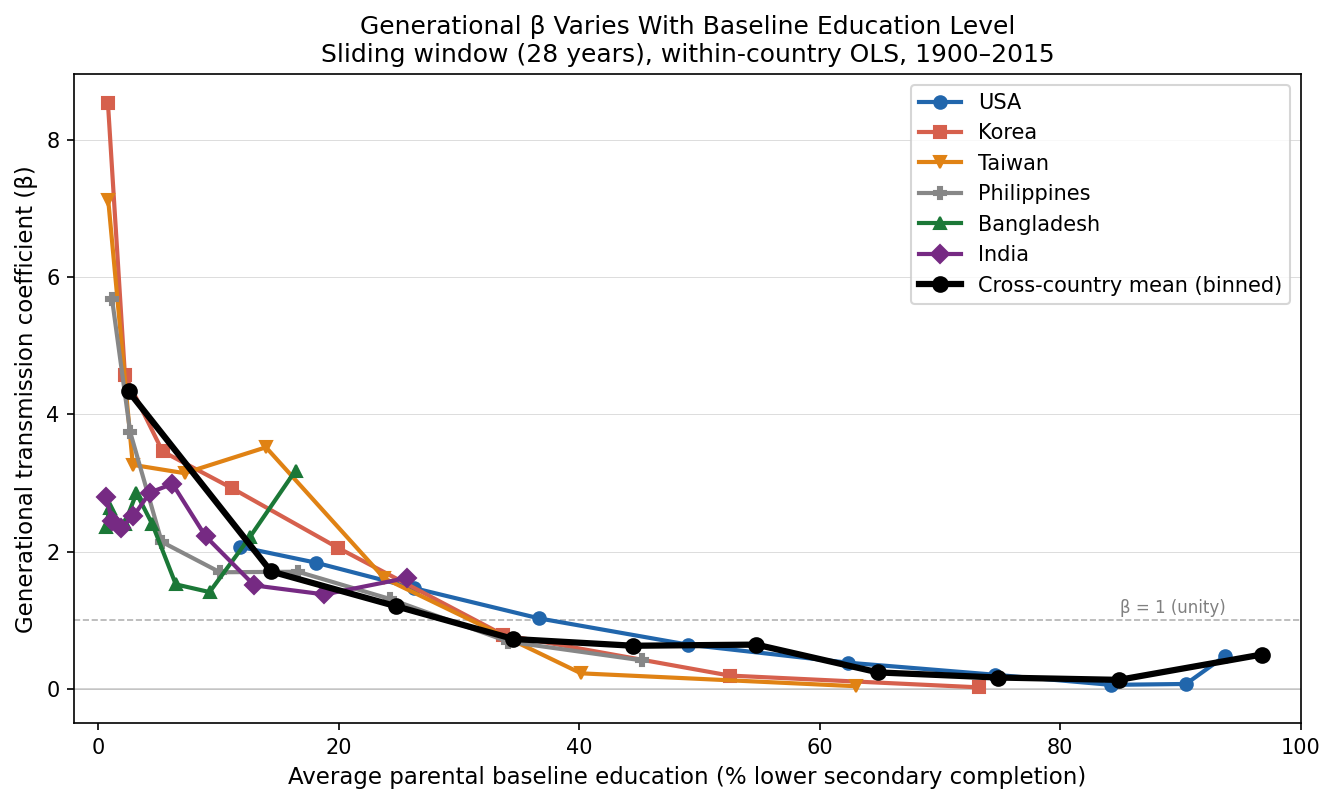
\includegraphics[width=\textwidth]{figures/beta_vs_baseline.png}
\caption[Generational $\beta_g$ versus baseline education level]{Generational $\beta_g$ varies systematically with baseline
education level. Each thin coloured line: 28-year sliding window
within one country, against the window's parental baseline. Thick
black line: cross-country mean across 185 countries
($n=1{,}312$ country-windows), binned by parental baseline. Illustrative
country trajectories (USA, Korea, Taiwan, Philippines, Bangladesh,
India) are labelled; the universality claim sits with the black
line. $\beta_g>1$ at low baselines reflects state reach; $\beta_g\to0$
reflects ceiling compression (WCDE v3 long-run cohort reconstruction
1875--2015; \texttt{scripts/wcde/long\_run\_generational.py}).}
\label{fig:beta-baseline}
\end{figure}

\paragraph{Quality vs.\ quantity in cross-section.}
The within-country panel (this section) shows lower-secondary
completion capturing $R^2 = 0.67$ for TFR (lag 5), $0.43$ for LE
(lag 12), and $0.46$ for U5MR (lag 12) --- the load-bearing evidence is
within countries as they expand schooling. A complementary 2015
cross-section ($n=66$--$67$ countries with HLO test-score data) races
lower-secondary completion against HLO cognitive quality on each
outcome. In the cross-section, HLO dominates: for TFR, lower-sec
$\beta_z = -0.19$ ($p = 0.14$), HLO $\beta_z = -0.51$ ($p < 0.01$);
for U5MR and LE the HLO edge is larger still
(Table~\ref{tab:composition}). HLO is not absorbed by adding
grandparent-generation lower-sec as a stock control: with lower-sec
at $T$, lower-sec at $T{-}28$, and HLO jointly, HLO's coefficient
holds at $\beta_z = -0.54$ ($p < 0.001$). Education quality, where
measured, is genuinely informative across all three outcomes. The
panel and the cross-section answer different questions --- "what
moves when a country expands schooling" versus "what differentiates
countries today" --- and lower-secondary coverage remains the
operational policy lever in both.

\refstepcounter{table}\label{tab:composition}\addcontentsline{lot}{table}{\protect\numberline{\thetable}Quantity vs.\ quality in 2015 cross-section}Table~\thetable: Quantity (lower-secondary completion) vs.\ quality (HLO) in 2015 cross-section.

{\small\setlength{\tabcolsep}{6pt}
\begin{longtable}[]{@{}lcccc@{}}
\toprule
Outcome ($T{=}2015$) & Quantity $\beta_z$ ($t$) & Quality $\beta_z$ ($t$) & Both-model $R^2$ & $n$ \\
\midrule
\endhead
TFR        & $-0.19$ ($-1.5$)\hphantom{**}    & $-0.51$ ($-3.4$)*** & 0.45 & 66 \\
log(U5MR)  & $-0.16$ ($-1.7$)\hphantom{**}    & $-0.70$ ($-7.6$)*** & 0.78 & 67 \\
LE         & $-0.12$ ($-1.1$)\hphantom{**}    & $+0.83$ ($+7.7$)*** & 0.62 & 67 \\
\bottomrule
\end{longtable}}\addtocounter{table}{-1}% undo longtable's auto-step (we use manual \refstepcounter for labels)

\begin{minipage}{\dimexpr\textwidth-2em}
\scriptsize
\textbf{Notes:} Cross-sectional 2015 horse race. All variables
standardised so $\beta_z$ is the per-standard-deviation response.
Quantity = lower-secondary completion at 2000 (the parent generation's
own 20--24 cohort education, WCDE v3); Quality = harmonised learning
outcome (HLO) test scores at secondary level from Angrist et
al.\ (2021). Both specifications include log population and HC1
robust SEs. $^{***}p<0.01$. The cross-section reflects between-country
variance; the within-country panel result (lower-sec captures $R^2 =
0.67$ for TFR at lag~5) carries the load-bearing claim. HLO is not
displaced by adding grandparent-generation lower-sec ($T{-}28$) as a
cumulative-stock control --- it captures something cross-country
distinct from accumulated coverage.
\textit{Produced by:}
\texttt{scripts/hanushek\_horse\_race\_comprehensive.py} and
\texttt{scripts/diagnostics/horse\_race\_with\_earlier\_cohort.py}.
\end{minipage}

Completion is the panel's operative variable because at population
scale the question is whether the child sat inside the channel long
enough for the categorical reorganisation to consolidate; the theory
of why completion measures exposure rather than learning is in
Chapter~\ref{categorical-brain-reorganisation}.

\paragraph{What rules out chance.}
A permutation null reshuffling the parent--child match across
countries (200 iterations) places the observed slope more
than 50 SDs above either null --- the within-year null, which
preserves global temporal trends, and the full shuffle, which
breaks every systematic link
(\nolinkurl{scripts/robustness/permutation_null.py}). Common
trends, panel autocorrelation, and serial correlation cannot
generate the coefficient by chance. Within countries male and female
lower-secondary completion expand together (within-country
correlation $>0.9$); the home niche moves as a unit, and the
country panel cannot decompose by sex. The cross-sectional
microdata literature locating the channel in mothers specifically
(Caldwell 1979; Schultz 2002; Jensen 2010; Duflo 2012) is
identified at the within-country individual level and is consistent
with the panel result: the channel is mother-weighted in routing
and household-located in measurement.

Non-depreciation of the channel under destructive disruption is
the Cambodia test (Section~\ref{cambodia-the-home-niche-shadow}).

\paragraph{GDP residualised: the null.}
Take each country's log GDP per capita and residualise out the part
that education produced (Frisch-Waugh-Lovell;
\texttt{scripts/residualization/education\_vs\_gdp.py}); use only what
remains to predict development outcomes. The residual predicts nothing
(Table~\ref{tab:residualisation}). This is not an artifact of which
variable is stripped: run the residualisation the other way --- take
education's unique contribution beyond GDP against GDP's unique
contribution beyond education --- and education's signal comes back
13.3$\times$ larger (the reverse-direction reading below), with a
symmetric permutation null confirming the asymmetry on every outcome.
Were the two merely collinear, both directions would return symmetric;
they do not.

\refstepcounter{table}\label{tab:residualisation}\addcontentsline{lot}{table}{\protect\numberline{\thetable}Residualised GDP analysis: education vs.\ log GDP per capita as predictors}Table~\thetable: Residualised GDP analysis -- education vs.~log GDP per capita as predictors.

{\footnotesize\setlength{\tabcolsep}{3pt}
\begin{longtable}[]{@{}lccccc@{}}
\toprule
Outcome ($T{+}\text{lag}$) & Edu $R^2$ & GDP $R^2$ & Resid GDP $\beta$ (SE) & Resid $p$ & Resid $R^2$ \\
\midrule
\endhead
Life expectancy   & 0.428 & 0.192 & \hphantom{$-$}0.160 (1.418) & 0.91 & \textbf{0.000} \\
Total fertility   & 0.669 & 0.292 & \hphantom{$-$}0.004 (0.324) & 0.99 & \textbf{0.000} \\
Child education   & 0.524 & 0.295 & \hphantom{$-$}2.845 (3.472) & 0.41 & \textbf{0.005} \\
Under-5 mortality & 0.457 & 0.170 & 2.933 (9.494)  & 0.76 & \textbf{0.001} \\
\bottomrule
\end{longtable}}\addtocounter{table}{-1}% undo longtable's auto-step (we use manual \refstepcounter for labels)

\begin{minipage}{\dimexpr\textwidth-2em}
\scriptsize
\textbf{Notes:} Entry-cohort design (entry $\geq$10\%, ceiling
$\leq$90\%); country FE; lower-secondary completion at $T$, outcome
at $T{+}\text{lag}$ where lag is biologically anchored per outcome
(TFR: lag $=$ LAG\_TFR, reproductive peak; LE and U5MR: lag $=$
childrearing window, LE being mortality-dominated; child-edu: lag
$=$ LAG\_GENERATION, the cross-generation step);
$T=1960$--$1990$;
country-clustered SE in parentheses. Residualised GDP is log GDP per
capita after Frisch-Waugh-Lovell residualisation against education.
Each outcome is on its own max-sample (sample sizes vary because
LE/TFR/U5MR/child-edu have different country-year coverage). The
residual-GDP null also survives restriction to the common intersection
sample across all four outcomes; that variant, along with the
unique-$R^2$, Maddison-backfilled, and ceiling-sweep variants, is in
\texttt{scripts/residualization/} and leaves the headline intact.
\textit{Produced by:} \texttt{scripts/residualization/education\_vs\_gdp.py},
\texttt{scripts/tables/regression\_tables.py}.
\end{minipage}

A 1-pp rise in lower-secondary completion at $T$ predicts, at each
outcome's biological lag, a gain of $+0.19$ years of life, $-0.058$
births per woman, and $1.33$ fewer under-five deaths per thousand; the
same-magnitude response to residualised log GDP is statistically
indistinguishable from zero in every row. Education explains 0.43 to
0.67 of within-country variation; the leftover-GDP $R^2$ is at most
0.019, and it stays there across the range of biologically plausible
lags, from the childrearing window out to a full generation
(\texttt{scripts/robustness/lag\_sensitivity.py}). Education
is doing essentially all the predictive work.
A country-resampling bootstrap and a full-shuffle permutation null
confirm the asymmetry directly: education's coefficient sits far outside
its null on every outcome, while residualised GDP --- education stripped
out of it --- sits inside its own
(\nolinkurl{scripts/robustness/permutation_null_symmetric.py}).

\paragraph{Why controlling for GDP is the wrong move.}
The prior is Prediction~\ref{pred:income}: GDP is the national-accounts
face of the Level-2 (literate-CT) regime, so residualised log GDP per
capita should have no independent predictive power once education's
contribution is stripped. The biology gives the direction; the panel
tests it. The educated population produces the GDP, so income is
downstream of education at every scale that matters: controlling for
GDP at the country-panel level controls for education running through
national accounts. The empirical claim is that once you stop doing that ---
strip GDP of education's contribution and use only the leftover ---
the leftover predicts nothing. The Asian Financial Crisis
(Section~\ref{the-shock-test}) shows the same separation in observable
time: GDP collapsed across five countries while lower-secondary
completion continued uninterrupted in every one. The shell
can be destroyed; the channel survives. The reverse-direction reading
sharpens it from the panel side: on the expansion sample ($n=537$),
parental-generation GDP alone predicts child education substantially
($\beta=19.5$, $R^2=0.335$), but adding parental education collapses
GDP's coefficient by 69\% to $\beta=6.1$ and adds only $R^2=0.021$
beyond education. Education's unique contribution beyond GDP is
$R^2=0.280$ --- 13.3$\times$ larger. GDP transmits through education,
not vice versa.

\paragraph{Robustness to baseline stratification.}
The pooled level-U5MR residGDP $\times$ Post-2000 interaction is
$+34.0$ ($p=0.022$); the pre-2000 within-country residGDP slope is
$-0.37$ ($p=0.018$). But the test that matters is whether residGDP
predicts mortality at a \emph{given} parental-education baseline, and
it does not: stratifying by parental lower-secondary completion, no
individual bin shows a residGDP coefficient that clears bootstrap
significance, and the within-bin meta-estimate's 95\% CI includes zero
at every one of the chapter's three timescales (full bin test,
bootstrap CIs, and composition detail in
\texttt{scripts/ECONOMETRICS.md}). The pooled signal is between-bin
composition: pre-2000 active-expansion cells sit at lower parental
completion than post-2000 cells, on a U5MR distribution that fell
sharply over the period. Within bins, given a country's parental
education, residual GDP does not predict mortality.

The Lutz and Kebede (2018) 1990--2010 child-mortality acceleration
is real. Vaccines, oral rehydration, vitamin A, IMCI, GAVI, the
MDGs delivered absolute reductions in deaths per thousand. The
acceleration runs through the schooled mothers of the 1970s and
1980s expansions reaching childbearing age and using those tools.

\subsection{The Shape of the Response}\label{the-shape-of-the-response}

Each outcome responds to lower-secondary completion at the lag where
its mechanism runs. Log GDP is contemporaneous --- the educated
worker contributes to output in the same year. A woman's own
fertility (TFR) follows about five years on, as her cohort reaches
its reproductive peak; her children's survival (U5MR) registers at
the childrearing window, about twelve years on. Life expectancy at
birth moves on that same childrearing clock --- lag~12 --- because it
is mechanically dominated by child mortality, not by a separate
adult-longevity channel a generation back. None
of these outcomes carries a clock of its own. They do not drift
upward with calendar time; they move when schooling moves, and they
have risen across the post-war decades only because schooling spread
across those decades. Time is not the cause --- education is --- and
the four outcomes co-move because the same lever drives each of them.
The panel evidence below is the within-country signature: as a
country expands lower-secondary, each outcome moves at its own lag.

\refstepcounter{table}\label{tab:edu-outcomes}\addcontentsline{lot}{table}{\protect\numberline{\thetable}Lower-secondary completion and development outcomes at canonical lag}Table~\thetable: Lower-secondary completion and development outcomes at canonical lag per outcome.

\noindent\textit{Panel A: Lower-secondary completion at $T$ $\to$ each outcome at its canonical lag (per \texttt{scripts/\_shared.py}): GDP at lag~0; LE at lag~12 (childrearing window); TFR at lag~5 (cohort at reproductive peak); U5MR at lag~12. Each row is one outcome; the coefficient is education-only. Adding contemporaneous log~GDP as a control barely changes any coefficient (Notes).}

{\small\setlength{\tabcolsep}{3pt}
\begin{longtable}[]{@{}lc@{}}
\toprule
Outcome (lag)         & Coefficient \\
\midrule
\endhead
log GDP (lag 0)       & +0.0185*** \\
                      & (0.0014)   \\
log(LE) (lag 12)      & +0.0042*** \\
                      & (0.0003)   \\
log(TFR) (lag 5)      & $-$0.0165*** \\
                      & (0.0005)   \\
log(U5MR) (lag 12)    & $-$0.0327*** \\
                      & (0.0014)   \\
\midrule
Country FE            & Yes \\
N (GDP row)           & 1{,}812 \\
N (LE row)            & 1{,}976 \\
N (TFR row)           & 2{,}155 \\
N (U5MR row)          & 1{,}575 \\
\bottomrule
\end{longtable}}\addtocounter{table}{-1}% undo longtable's auto-step (we use manual \refstepcounter for labels)

\begin{minipage}{\dimexpr\textwidth-2em}
\scriptsize
\textbf{Notes:} Each outcome regressed on lower-secondary completion
at $T$ at its canonical lag per \texttt{scripts/\_shared.py}: log
GDP at lag~0 (\texttt{LAG\_CONTEMPORANEOUS}); LE at lag~12
(\texttt{LAG\_LE}, childrearing window); TFR at lag~5
(\texttt{LAG\_TFR}, cohort at reproductive peak); U5MR at lag~12
(\texttt{LAG\_CHILDREARING}). Country FE throughout;
country-clustered SE in parentheses; $^{*}p<0.10$, $^{**}p<0.05$,
$^{***}p<0.01$. Coefficients are semi-elasticities (proportional
change in outcome per pp rise in lower-secondary completion).
Adding contemporaneous log~GDP at $T$ as a control barely moves any
coefficient: LE $+0.0039$ (0.0004), TFR $-0.0153$ (0.0008), U5MR
$-0.0290$ (0.0021), on the GDP-merged samples (N $=$ 1{,}633 / 1{,}812
/ 1{,}253 respectively); the log~GDP row is unchanged because the
outcome is itself log~GDP. The
cross-generation ($T{+}28$) variant is retained as a
forward-prediction identification robustness; see
Section~\ref{gdp-has-no-independent-effect} for the reverse-direction
check (GDP at $T$ predicting child education at $T{+}28$).
\textit{Produced by:} \texttt{scripts/wcde/table\_contemporaneous.py}.
\end{minipage}

Reading Panel~A: each 1-pp gain in lower-secondary
completion at $T$ predicts, each outcome at its biological lag
(Notes), 1.85\% higher GDP per capita (lag~0), 0.42\% higher life
expectancy ($\approx$0.29 years at $\text{LE}=70$; lag~12), 1.65\%
lower TFR ($\approx$0.06 fewer children per woman at
$\text{TFR}=3.5$; lag~5), and 3.27\% lower under-five mortality
(lag~12). All four are within-country
effects; every Panel~A coefficient is significant at
$p<0.01$. Across the four outcomes the predictor's coefficient barely
moves once log~GDP enters as a control (Notes) --- the
population-scale signature that GDP is downstream of education, not a
parallel channel.

\paragraph{Four generations of reach.} Figure~\ref{fig:lag-100} extends
the lag-28 finding to four generations. The standardised within-country
$|\beta|$ for lower-secondary completion predicting each outcome
decays smoothly from lag 28 through lag 112; every outcome remains
significant at $p<0.001$ at four-generation depth (minimum $|t|=5.9$, TFR).
Under-5 mortality carries the deepest signature ($|\beta|=0.331$ at
lag 112, $|t|=24.4$); LE, TFR and child education show the same
smooth monotonic decay. No other input has comparable reach: log GDP
per capita's $R^2$ falls below education's by lag 20--25 and cannot
be tested past lag $\sim$45 on raw WDI data, by construction --- the
pre-1960 subsistence baseline ($\sim$\$400--600 constant 2015 USD) has
no cross-country variation to test before literate populations
existed. The construction-bounded backfill check is in
\texttt{scripts/robustness/backfill\_all\_outcomes.py}.

\begin{figure}[htbp]
\centering
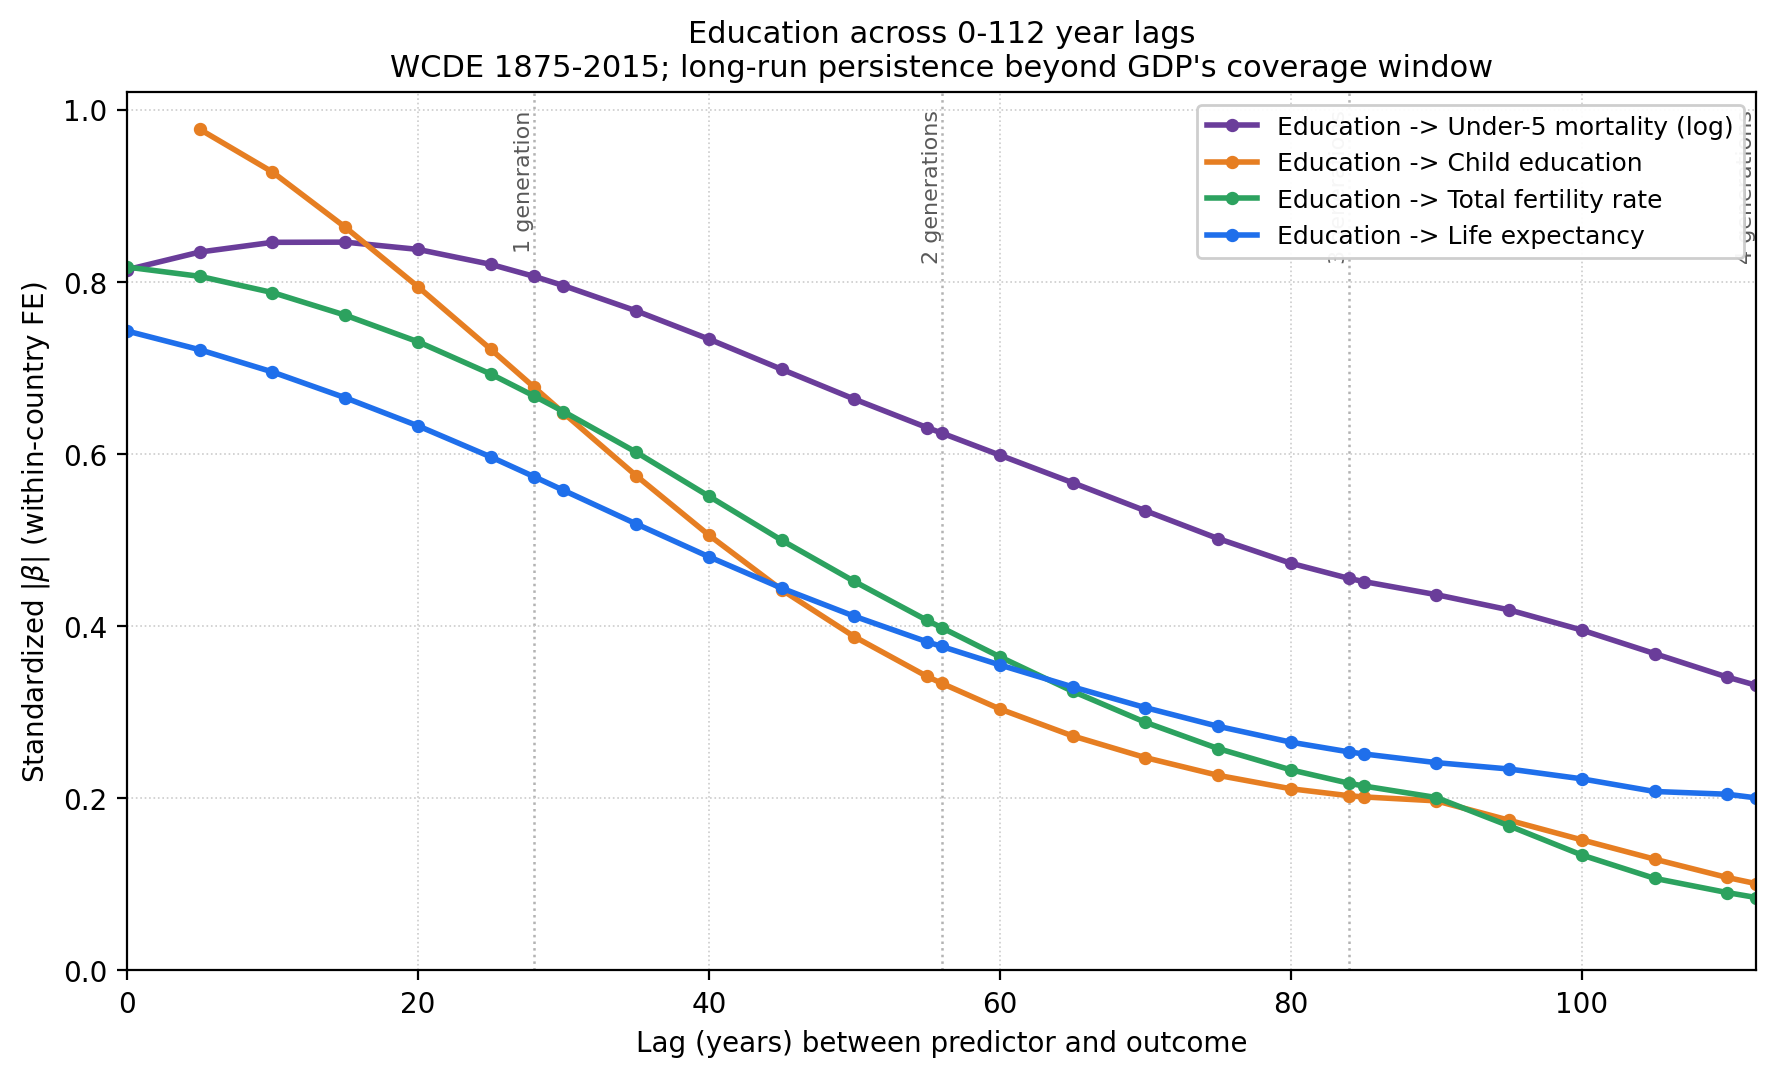
\includegraphics[width=\textwidth]{figures/outcomes_beta_by_lag_4b.png}
\caption[Education across lags 0--112 years]{Education across lags 0--112 years.
Standardised within-country $|\beta|$ for lower secondary completion
predicting four development outcomes, extended to four-generation
depth (WCDE v3 cohort reconstruction 1875--2015). Generational
horizons 1--4 marked.}
\label{fig:lag-100}
\end{figure}

\subsection{The Grandparent Channel}\label{the-grandparent-channel}
Does the grandparent's education predict outcomes \emph{independently}
of the parent's? Under biological anchoring --- parent education at
$T-5$ (the parental cohort at reproductive peak in the outcome year)
and grandparent education at $T-33$ --- both channels carry
independent, highly significant signals on fertility everywhere in
the panel. In the full panel $\beta_p=-0.050$ and $\beta_{gp}=-0.011$
(both $p<0.01$; $n=1216$, 152 countries); within-$R^2$ rises from
0.56 to 0.59 once grandparent education is added. Restrict to
countries where parental completion is below 50\% and both
coefficients grow: $\beta_p=-0.068$, $\beta_{gp}=-0.048$ (both
$p<0.001$; $n=464$, 80 countries); within-$R^2$ jumps from 0.69 to
0.74. The parent's coefficient is everywhere larger; the
grandparent's coefficient never collapses to zero. The largest
grandparent signal is on child survival (U5MR, at the childrearing
lag --- parent at $T{-}12$, grandparent at $T{-}40$): in the full
panel $\beta_{gp}=-0.020$ on log U5MR, slightly larger in absolute
terms than the parent's ($\beta_p=-0.018$); within-$R^2$
rises from 0.407 to 0.653 once grandparent education is added
($n=825$, 165 countries). Table~\ref{tab:grandparent} collects the
cited coefficients.

\refstepcounter{table}\label{tab:grandparent}\addcontentsline{lot}{table}{\protect\numberline{\thetable}Grandparent channel: parent-only vs.\ parent + grandparent}Table~\thetable: Grandparent channel --- parent-only vs.\ parent + grandparent education.

{\footnotesize\setlength{\tabcolsep}{3pt}
\begin{longtable}[]{@{}lccccc@{}}
\toprule
Outcome (sample) & Parent-only $\beta_p$ & + GP: $\beta_p$ & + GP: $\beta_{gp}$ & within-$R^2$ & $n$ (ctry) \\
\midrule
\endhead
TFR (level, parent $<$50\%) & $-0.096$*** & $-0.068$*** & $-0.048$*** & 0.69$\to$0.74 & 464 (80) \\
log U5MR (full panel)       & $-0.033$*** & $-0.018$*** & $-0.020$*** & 0.41$\to$0.65 & 825 (165) \\
\bottomrule
\end{longtable}}\addtocounter{table}{-1}% undo longtable's auto-step (we use manual \refstepcounter for labels)

\begin{minipage}{\dimexpr\textwidth-2em}
\scriptsize
\textbf{Notes:} Grandparent (GP) education predicts outcome via the
biologically appropriate lag per outcome: for TFR, parent at $T-5$
(parental cohort at reproductive peak in the outcome year) and
grandparent at $T-33$; for U5MR, parent at $T-12$ (childrearing
window) and grandparent at $T-40$. Country FE; country-clustered
SE. The TFR row uses lower-secondary completion in levels on the
low-baseline subsample (parent completion $<50\%$); the U5MR row uses
log U5MR on the full panel. Parent and grandparent
education are drawn from the same within-country series and are
structurally correlated: in a country undergoing sustained expansion
both regressors trend together, so the marginal grandparent signal
collapses once parental baselines saturate. The low-baseline
restriction in the TFR row isolates the regime where they vary enough
to separate.
$^{**}p<0.05$, $^{***}p<0.01$.
\textit{Produced by:} \texttt{scripts/robustness/grandparent\_effect.py},
\texttt{scripts/robustness/grandparent\_effect\_all\_outcomes.py}.
\end{minipage}

The pattern is what the
generational gate predicts: at low baselines each educated person in
the household adds independent weight; at high baselines the parent
has internalised everything the grandparent could offer. This
generates a falsifiable prediction the panel cannot test directly: any
educated elder inside the child's kin/community radius (co-resident
grandparent, aunt, village exemplar) should raise grandchild outcomes
beyond what the parent's education predicts; equivalent elders
present only on paper (deceased, non-resident) should not. DHS
co-residence data can test it.

\subsection{Universality Across Subsamples}\label{universality-across-subsamples}

The mechanism is universal --- and universal in a stronger sense than a
stable coefficient. A relationship that stays positive in every region
shows it does not vanish anywhere; it does not, by itself, show the same
mechanism runs everywhere, since unlike pathways can each yield a
positive slope. The test is whether the \emph{whole signature} repeats:
not one coefficient but the coordinated response of all four outcomes,
each at its own biological lag. It does. Two tests, panel and residual.

\emph{Panel, eleven subsamples.} Re-estimating Column~1 of
Table~\ref{tab:headline} on eleven subsamples (six regions, two
child-cohort eras, three within-sample GDP terciles) produces eleven
positive coefficients, every one significant at $p<0.01$, with $\beta$
ranging from 1.258 (Middle East \& N.~Africa, n=67) to 2.562 (South
Asia, n=58). Sub-Saharan Africa, where most of the remaining 20\% of
humanity sits, returns $\beta=1.270$ (SE 0.144, $R^2=0.692$, n=312,
40 countries) --- tracking the full-sample headline. Re-estimating not
that single coefficient but the full per-outcome specification
(Table~\ref{tab:edu-outcomes}: lower-secondary completion at $T$ $\to$
log GDP at lag~0, log~TFR at lag~5, log~LE and log~U5MR at lag~12) on the
same eleven subsamples reproduces the entire signature: in every
subsample GDP rises, fertility falls, life expectancy rises, and child
mortality falls, each at its canonical lag --- all 44 coefficients
(eleven subsamples $\times$ four outcomes) carrying the predicted sign
and significant at $p<0.01$. A different mechanism in each region could
not produce one coordinated four-outcome pattern at the same four lags
everywhere. Era and tercile
splits rule out post-Cold-War and income-band artefacts. The
universality claim is also tested on the institutional literature's
own preferred sample: on AJR's (2001) 64-country former-colony base,
colonial-era education explains a near-identical share of log GDP
variance as AJR's \emph{avexpr} institutional measure
(Chapter~\ref{what-every-framework-was-reaching-for},
\S\ref{the-institutional-challenge}), and the settler-mortality
instrument identifies the educational channel as well as the
institutional one.

\emph{Residuals, eight over-performers.} Some countries are educating
children far beyond what their parents' generation would predict.
Country fixed-effects residuals from a within-country regression of
child on parent lower-secondary completion at the 28-year lag, using
the full child-education panel (1875--2015, 185 countries), identify
eight at $T{+}28 = 2015$: they are uniformly poor.

\refstepcounter{table}\label{tab:over-performers}\addcontentsline{lot}{table}{\protect\numberline{\thetable}Education over-performers (2015 FE residuals)}Table~\thetable: Education over-performers (2015 FE residuals).

\begin{longtable}[]{@{}lll@{}}
\toprule
Country & FE residual above baseline & GDP per capita (2015) \\
\midrule
\endhead
Maldives & +37.2 pp & \$9,645 \\
Bhutan & +25.5 pp & \$2,954 \\
Cape Verde & +24.9 pp & \$3,415 \\
Viet Nam & +22.6 pp & \$2,578 \\
Tunisia & +20.8 pp & \$4,015 \\
Nepal & +17.9 pp & \$876 \\
Bangladesh & +17.5 pp & \$1,224 \\
India & +14.9 pp & \$1,584 \\
\bottomrule
\end{longtable}\addtocounter{table}{-1}% undo longtable's auto-step (we use manual \refstepcounter for labels)

\begin{minipage}{\dimexpr\textwidth-2em}
\scriptsize
\textbf{Notes:} Each within-country residual is
child lower-secondary completion at $T{+}28$ minus the within-country
slope $\hat{\beta}$ multiplied by parent completion at $T$, country-demeaned;
$\hat{\beta}$ is estimated by country fixed-effects OLS across the
\emph{full} child-education panel (1875--2015, all 185 countries),
not the active-expansion sample of Table~\ref{tab:headline}. The figure reported is each
country's residual at $T=1990$ --- child cohort observed in 2015. The
residual measures deviation from the country's own historical trend
predicted by the within-country slope. It is not a comparison against
other countries at similar income, region, or other observables; a
country can be a positive residual here simply because its child
generation rose faster relative to its own parents than the panel
slope predicts.
\textit{Produced by:} \texttt{scripts/tables/regression\_tables.py}.
\end{minipage}

Nepal at \$876 (2015), Bangladesh at \$1,224, Vietnam at \$2,578.
Income is not the prerequisite for educational over-performance. The
robustness battery (alternative cutoffs, lag lengths, PPML, balanced
subpanel, Barro-Lee replication, the 20-test econometric battery) is
in \texttt{scripts/} (Section~\ref{what-the-panel-supports}).
None reverses the ordering, and no check reduces the education/GDP
$R^2$ ratio below 2.1$\times$.

\subsection{Every Method Agrees}\label{every-method-agrees}

The within-country panel above used ordinary least squares with country
fixed effects. A reader trained in econometrics will ask how much of the
education-load-bearing result depends on that one functional form. To
answer without leaning on a single estimator, I ran the same prediction
problem --- features at $T$ predicting outcomes at the canonical lag ---
through a spread of model classes under country-clustered five-fold
cross-validation: countries, not observations, are split across folds,
so every scored country is fully unseen in training. Each method's
education contribution is the drop in out-of-fold $R^2$ when the
education feature block is zeroed at inference.

The within-fixed-effects estimator itself cannot be cross-validated this
way --- a held-out country's fixed effect is unidentified, so the linear
class is represented by its regularised members, ridge and lasso. To
those I add two tree ensembles and a universal transformer encoder
trained with no country identity in its inputs, so it cannot memorise a
single country.

\refstepcounter{table}\label{tab:spec-curve}\addcontentsline{lot}{table}{\protect\numberline{\thetable}Education's out-of-fold $R^2$ contribution across five model classes}Table~\thetable: Education's out-of-fold $R^2$ drop when the education block is removed, country-clustered five-fold, each outcome predicted at its biological lag (LE@12, TFR@5, U5MR@12) on its own single-target panel.

{\small\setlength{\tabcolsep}{6pt}
\begin{longtable}[]{@{}lccc@{}}
\toprule
Method & $\Delta R^2$ (LE) & $\Delta R^2$ (TFR) & $\Delta R^2$ (U5MR) \\
\midrule
\endhead
Ridge (CV-tuned)      & 0.195 & 0.252 & 0.245 \\
Lasso (CV-tuned)      & 0.256 & 0.360 & 0.273 \\
Random forest         & 0.222 & 0.353 & 0.400 \\
Gradient boosting     & 0.191 & 0.330 & 0.367 \\
Universal transformer & 0.234 & 0.262 & 0.394 \\
\bottomrule
\end{longtable}}\addtocounter{table}{-1}

\begin{minipage}{\dimexpr\textwidth-2em}
\scriptsize
\textbf{Notes:} Out-of-fold $R^2$ drop from zeroing the education block
(WCDE current and cohort-historical attainment, Barro--Lee shares,
derived gender-gap terms). Each outcome is predicted at its own
biological lag (LE@12 via \texttt{LAG\_LE}, TFR@5, U5MR@12) on a
single-target panel. Transformer values are medians across 30 seeds;
the linear and tree methods are single CV-tuned fits.
Country-clustered folds throughout. \textit{Produced by:}
\texttt{scripts/ml/chapter9/spec\_curve.py~--parent} and
\texttt{aggregate\_parent\_vantage.py}.
\end{minipage}

The five rows return the same answer. Education's out-of-fold
contribution stays in the same band across every estimator, and the
transformer --- which imposes no functional form and cannot memorise a
country --- sits inside that band rather than above or below it. The
result is not an artifact of the panel's estimator.

\paragraph{Education against income, head to head.} The cleanest single
cut pits education against its main rival. I trained the transformer on
the full feature set, then ablated one block at a time and measured the
loss in held-out accuracy. Removing education costs the model between a
third and over half of its held-out accuracy --- $0.31$ for life
expectancy, $0.31$ for fertility, $0.52$ for under-five mortality.
Removing GDP costs almost nothing --- $0.02$, $0.002$, and $0.007$ for
the same three. On unseen countries, with no functional form imposed,
education does an order of magnitude more work than income.

\paragraph{What these methods establish.} Across estimators that impose
no shared functional form, education's population-scale contribution
survives every guard against overfit, country memorisation, and chance.
The biology and the natural experiments establish the channel; this
battery confirms that its signature is real. The placebo falsifications
(six transformations, including replacing education with absolute
latitude), the out-of-fold country counterfactuals, the
double-machine-learning causal estimate, the walk-forward projection,
and leave-one-out fits are in \texttt{scripts/ECONOMETRICS.md}.

\subsection{What the Panel Supports}\label{what-the-panel-supports}

The variables the channel's signature is read in are not the contested
kind, and the country is not the unit that matters in them. Fertility, life
expectancy, and length of life are counts of what individual bodies do
--- each birth, each survival, each life a separate realisation of the
same mechanism running in the same organism. A country-year rate is only
the tally of millions of those bodies inside an administrative boundary
the biology does not recognise; the evidence is the bodies, and they
number in the billions across every region and era. This is the register
of medicine, not of the cross-country regression: a mechanism fixed in
the human organism is established on the organism --- at the within-country
individual level (Chapter~\ref{generational-transmission-and-state},
Section~\ref{the-deaton-objection}) --- and holds for the
species, as a clinical finding holds for every human without being
re-run nation by nation. The panel collapses those billions into country
rates because the country is the unit the data exists in, not the unit the mechanism lives in --- which is
why it is the translation and not the proof; the proof's reach is the
species, and the count of countries is an artifact of the lens.

The
chapter reads those population-scale signatures rather than estimating a
treatment effect --- signatures of a structural channel that
Chapters~\ref{longest-juvenile-dependency}--\ref{generational-transmission-and-state}
deduce and Chapters~\ref{natural-experiments}--\ref{country-histories}
identify in observable time. The natural experiments in
Chapter~\ref{natural-experiments}, the country histories in
Chapter~\ref{country-histories}, and the USSR falsification in
Chapter~\ref{hollow-education} are the rigorous work.
Section~\ref{education-as-limiting-factor} gives the structural
reason no other variable could have carried the panel signature: the
cognitive substrate is loadable only during the juvenile dependency
window, and education is the only intervention that loads it;
institutions, markets, and technology act on adults already formed.
The standard toolkit --- two-way fixed effects, instrumental
variables, the marginal-control battery --- is built for a different
question; Section~\ref{methodological-frontier} sets out why it runs
downstream of this channel rather than reaching it. The reader who wants to push on the panel will find every
specification, robustness check, and variant in \texttt{scripts/} on
GitHub, indexed by \texttt{scripts/ECONOMETRICS.md}:
common-sample, Maddison-backfill, and ceiling-sweep variants of
the residualisation; the country-shuffle permutation null; and the
20-test panel-diagnostic battery --- including the staggered-adoption
DiD, IV contests, and TWFE diagnostics run for completeness.

\section{Hollow Education: What the Soviet Anomaly Tests}\label{hollow-education}

The mechanism predicts: if a population is reported to be educated but does not actually undergo categorical reorganization in the childhood window, then fertility and mortality will not shift to match the reported education. The Soviet 15 provide the natural experiment.

The paper's empirical engine is lower-secondary completion --- the
floor at which the cultural-transmission regime begins acting
through household decisions
(Section~\ref{why-lower-secondary-completion}). I take the series
from the WCDE v3 reconstruction (Lutz et al.\ 2021) because it
reaches back to 1875 on a consistent definition and passes the
phenotype tests laid out in Section~\ref{phenotype-test-ussr}. On the 185-country panel,
WCDE reports near-universal lower-secondary completion for the
fifteen Soviet republics by 1970.

But that near-universal reporting masks two different realities, and
the cleanest witness to the gap is fertility. A pro-natalist state
that awarded medals for large families had no reason to fake its birth
rates down, so fertility alone reports truthfully on the schooling.
The eight republics east or south of Moscow (Georgia, Armenia,
Azerbaijan, Turkmenistan, Uzbekistan, Tajikistan, Kyrgyzstan,
Kazakhstan) carry fertility that tracks their low-education neighbours,
not their reported credential; the six republics to the west (Belarus,
Ukraine, Lithuania, Latvia, Estonia, Moldova) carry fertility that
matches the schooling they report. The split is categorical, not a
gradient, and it falls at Moscow's longitude (Section~\ref{moscow-meridian}).

Child mortality reproduces the same line, but as the conservative
witness rather than the clean one. A state that inflates its schooling
deflates its mortality by the same hand: in rural Central Asia Soviet
child mortality was reported three to four times too low, and old-age
survival inflated by age exaggeration (Anderson \& Silver 1986). The
under-five residuals that locate the anomaly therefore understate the
true gap, not invent it --- and even understated, they fall exactly
where fertility does. The six western republics sit within
$\pm 1\sigma$ of the global education-phenotype fit on log U5MR; the
seven eastern republics with multi-year data sit 2.6 to 4.0$\sigma$
above what their reported lower-secondary completion predicts
(Uzbekistan's series begins only in 2020; Table~\ref{tab:moscow-meridian}).
Belarus at 629 km west of Moscow shows a U5MR residual of
$+0.43\sigma$; Georgia at 451 km east shows $+2.58\sigma$. Crossing the
Moscow meridian moves a republic from ``consistent with reported
education'' to ``phenotype catastrophically inconsistent with reported
education'' in a single jump.

The chapter treats this as a diagnostic, not a footnote. It is a
natural experiment run in reverse: the input side is corrupted, and
the corruption pattern reveals the social geography of the corrupting
institution. The Soviet metropole reported European-core educational
standards uniformly across its empire. Where the underlying
population was European-core --- Slavic west, Lutheran-Catholic
Baltics --- the report was approximately true. Where the underlying
population was Muslim or Caucasian periphery, the report was
metropolitan fiction.

In the childhood frame, hollow education is exactly this: the
eighteen-year window did not get loaded with the cognitive
architecture the schooling was supposed to install --- whether
because the schooling was thin, the attendance partial, or the
credential itself fictional over a population the state could not
see. The credential measures only what was reported; the phenotype
measures what entered the window.

The diagnostic yields three payoffs. First, a credibility case for
the panel: the active-expansion screen and the hollowness flag
independently exclude the same fifteen republics, so the headline
results are robust to USSR exclusion by construction. Second, a
reconciliation with the
Hanushek--Woessmann ``knowledge capital'' line (2008, 2012): the HLO
test-score measure, which the field has read as an alternative to
completion-based education, turns out to be a multi-generation
integrated output of completion itself. Third, a sharpened thesis on
what schooling transmits. The cognitive architecture loaded in the
dependency window is what produces the development response in TFR
and LE --- and, through the same mechanical link, in under-five
mortality; the credential without the phenotype does not. Hollow
education is not education.

\subsection{The Anomaly}\label{the-anomaly}

Of the 154 countries that have crossed the developmental threshold
by 2022, 24 were post-socialist --- 13 USSR republics plus 11 Warsaw
Pact and Yugoslav successors. The post-socialist crossers follow a
pattern nothing else in the panel matches. Among market-economy
crossers, the median country reached 90\% lower-secondary completion
16 years \emph{before} crossing the developmental threshold. Among
post-socialist crossers, the median country reached 90\% at the
crossing year. Among the USSR core, Turkmenistan crossed 57 years
after the reported date at which it reached 90\%. Either these
republics had reached 90\% decades before their fertility and
longevity trajectories responded --- a 50-year mechanism gap with no
precedent --- or the 90\% was not what it claimed to be.

The rest of the chapter tests the second hypothesis. Under the
paper's mechanism, reported education at year $T$ should produce a
phenotypic response within a generation, each outcome at its own
biological lag. Where it does not, either the
mechanism is wrong or the reported education is wrong. The mechanism
passes across the panel outside one bloc: 171 of the 185 countries
behave as it predicts, and the 14 Soviet republics with a phenotype to
test (Uzbekistan drops out of the panel on data coverage) share a
single origin --- one statistical office. Within that bloc the test
does not break uniformly; it splits the republics at Moscow's
longitude, as the chapter opening previewed. The European-core
republics to the west show the phenotypic response their reported
education predicts, while the republics to the east and south do not
(Section~\ref{moscow-meridian}). The failure is the periphery the
metropole could not see, not the credential itself.

\subsection{What WCDE Reports vs What Was Observable}\label{what-wcde-reports}

Three ground-truth checks against contemporaneous non-Soviet
neighbors --- Iran, Turkey, Afghanistan, Pakistan --- with comparable
pre-1917 educational baselines:

\textbf{Gender parity in 1970.} Central Asia reports a mean
female-minus-male lower-secondary completion gap of $-2.7$ pp (near
parity). Iran, Turkey, Afghanistan, and Pakistan report a mean gap
of $-15.6$ pp, with several countries at $-11$ to $-18$ pp.
Near-parity in 1970 rural Central Asia, with no comparable
pre-Soviet mass-schooling infrastructure, diverges sharply from
what comparable-baseline societies were producing the same decade. The
Baltics' reported near-parity is plausible (pre-1940 European
educational infrastructure); the Central Asian figure is not.

\textbf{Primary minus lower-secondary.} By construction, primary
completion must exceed lower-secondary completion: one cannot
complete the latter without the former. In 1980, non-Soviet neighbors
show a mean primary-minus-lower-secondary gap of $+21.0$ pp --- a fifth of the
cohort completes primary without continuing to lower-secondary.
Central Asia shows $+1.6$ pp: virtually every child who completes
primary is reported as completing lower-secondary as well. This
holds across individual Central Asian republics. Near-complete
continuation is not what normal school systems produce; it is what
uniform reporting produces.

\textbf{Raw 1970 levels.} Kazakhstan 94\%, Turkmenistan 95\%,
against Iran 22\%, Turkey 22\%, Pakistan 16\%, Afghanistan 6\%. A
70-percentage-point gap from comparable pre-1917 baselines, built in
half a century, is not what rural agricultural populations produced
in this period anywhere else on the planet. Later cognitive evidence
is consistent: Kyrgyzstan's 2009 PISA score of 350 sits at the low
end of the global distribution; Turkmenistan, Uzbekistan, and
Tajikistan do not participate in international assessments; Baltic
PISA scores at 500--535 are consistent with their reported
education and with separate pre-1940 educational infrastructure.

\subsection{The Phenotype Test}\label{phenotype-test-ussr}

The mechanism predicts that educational input at $T$ produces
phenotypic output within a generation, each outcome at its own
biological lag. Where disruption and lag are excluded, as they are
here, absent output isolates the input: the reported education did
not occur, or occurred empty of content.
Figure~\ref{fig:ca-vs-iran} shows the test for under-5 mortality.

\begin{figure}[H]
\centering
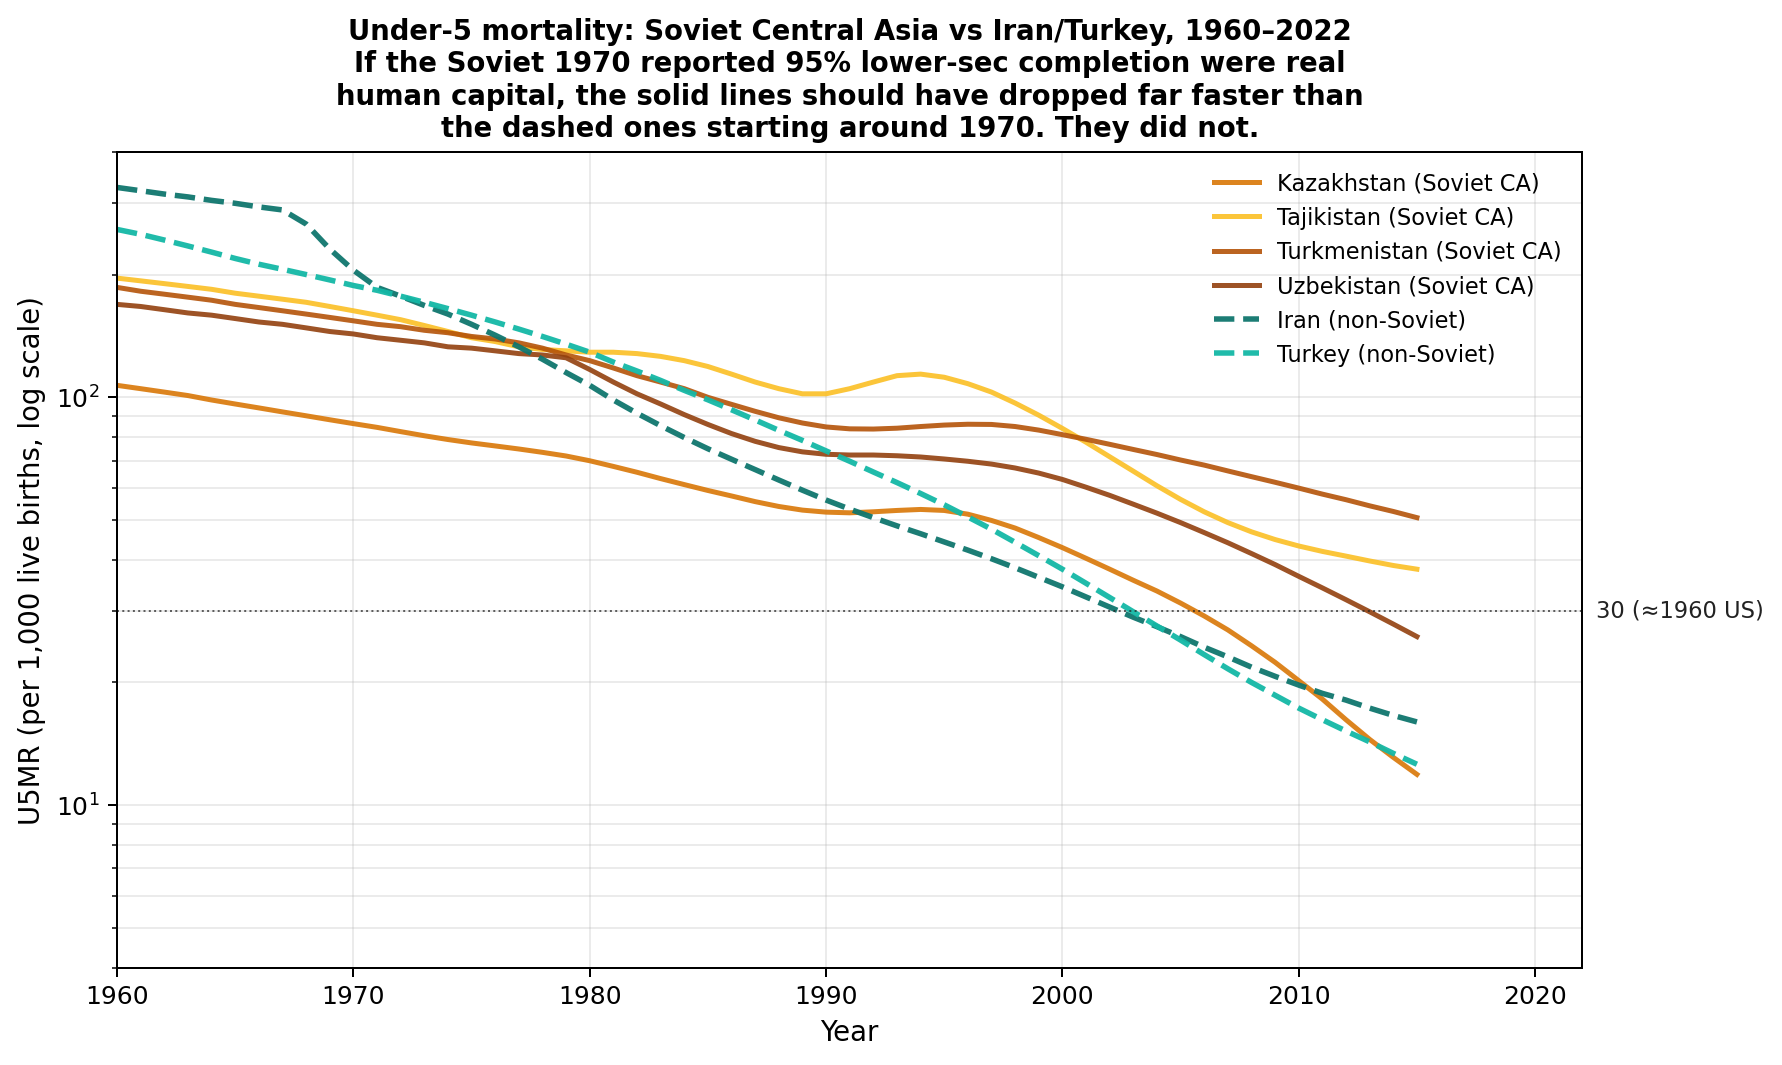
\includegraphics[width=0.95\linewidth]{figures/central_asia_vs_iran_turkey_u5mr.png}
\caption[Under-5 mortality trajectories, 1960--2010]{Under-5 mortality trajectories, 1960--2010. Central Asian
and Slavic USSR republics (colored lines) start 1960 with large
U5MR head starts over Iran (327 per 1,000) and Turkey (258). By
2010, Iran (20) has overtaken every Central Asian country except
Kazakhstan. Under the mechanism, the country with four times the
reported education in 1970 should dominate its neighbor permanently;
no later catch-up should be able to reverse a head start built on
five-times-larger secondary completion. The crossover says the head
start was not real. \emph{(Source: World Bank WDI.)}}\label{fig:ca-vs-iran}
\end{figure}

Iran 1960 $\to$ 2010: 327 $\to$ 20 per 1,000 (94\% decline).
Kazakhstan 1960 $\to$ 2010: 107 $\to$ 20 (81\% decline). Turkey 2010
at 17 beats every Central Asian country, Kazakhstan included. If the
1970 Soviet 95\% had been real, Central Asia should have dominated
Iran and Turkey permanently. But the head start was partly a reporting
artifact: the Soviet live-birth definition excluded the most fragile
newborns, understating infant mortality by 22--25\% empire-wide and by
a factor of three to four in rural Central Asia, where deaths went
unregistered or were misattributed to the second year of life
(Anderson \& Silver 1986). The reported 107 was a floor; the true
figure was far higher. What arrived after 1991 was not a Central Asian
collapse but honest counting --- Iran did not overtake the periphery so
much as the periphery's numbers stopped being made. Iran and Turkey are running on
school systems that delivered actual cognitive skill to the mothers
whose children survived.

TFR tells the same story more quietly. Central Asian fertility
trajectories from 1960 onward are indistinguishable from Iran's and
Turkey's. There is no 1991 kink --- the trajectories run smoothly
through Soviet dissolution as if the state had had no independent
effect on the household decision. What moved was the same thing
that moved in Iran: mothers becoming literate in their own dialect,
one generation ahead of the crossing.

The fertility test isolates the anomaly to one place, not to an
ideology. Under WCDE the Central Asian and Caucasian republics carry
a $+2.0$ SD fertility residual against the global fit, while the
Slavic republics, the Baltics, the Warsaw Pact, and Yugoslavia all sit
within a quarter of a standard deviation --- their fertility matches
their reported schooling. The anomaly is not socialism; it is the
metropole reporting on populations it could not see.

\subsection{The Moscow Meridian}\label{moscow-meridian}

The fifteen Soviet republics split categorically at Moscow's
longitude. Table~\ref{tab:moscow-meridian} shows the per-country
phenotype residual against the global non-USSR fit (lower-secondary
completion at $T$ predicting LE and log U5MR at $T$, 1960--2020),
ordered by signed east-of-Moscow distance.

\refstepcounter{table}\label{tab:moscow-meridian}\addcontentsline{lot}{table}{\protect\numberline{\thetable}Phenotype residual per Soviet republic vs east-of-Moscow distance}Table~\thetable: Phenotype residual per Soviet republic vs east-of-Moscow distance, WCDE lower-secondary completion age 20--24, global non-USSR fit.

{\small\setlength{\tabcolsep}{4pt}
\begin{longtable}[]{@{}lrrr@{}}
\toprule
Republic & East-of-Moscow (km) & LE residual ($\sigma$) & log U5MR residual ($\sigma$) \\
\midrule
\endhead
Latvia            & $-844$  & $-1.06$ & $+0.75$ \\
Estonia           & $-804$  & $-0.89$ & $+0.57$ \\
Lithuania         & $-771$  & $-0.81$ & $+0.35$ \\
Belarus           & $-629$  & $-0.96$ & $+0.43$ \\
Moldova           & $-547$  & $-1.41$ & $+1.87$ \\
Ukraine           & $-444$  & $-0.95$ & $+1.09$ \\
Russia (metropole) & $0$    & $-1.40$ & $+1.13$ \\
Armenia           & $+431$  & $-1.42$ & $+2.77$ \\
Georgia           & $+451$  & $-1.51$ & $+2.58$ \\
Azerbaijan        & $+765$  & $-2.20$ & $+3.63$ \\
Turkmenistan      & $+1{,}291$ & $-2.31$ & $+4.00$ \\
Tajikistan        & $+1{,}934$ & $-2.20$ & $+3.73$ \\
Uzbekistan        & $+1{,}961$ & $-1.00$ & $-{}^{a}$ \\
Kyrgyzstan        & $+2{,}285$ & $-1.80$ & $+3.23$ \\
Kazakhstan        & $+2{,}422$ & $-1.90$ & $+2.69$ \\
\bottomrule
\end{longtable}}\addtocounter{table}{-1}% undo longtable's auto-step (we use manual \refstepcounter for labels)

\begin{minipage}{\dimexpr\textwidth-2em}
\scriptsize
\textbf{Notes:} Residuals are mean of country-year residuals against
the global non-USSR education-phenotype fit at each year, scaled by
the year-specific residual standard deviation. East-of-Moscow distance
is the great-circle distance along the parallel through Moscow,
signed positive eastward. $^{a}$Uzbekistan's WCDE lower-secondary
data covers only year 2020, no overlap with U5MR.
\end{minipage}

Three readings.

\textit{The west-east discontinuity.} The six westward republics
show U5MR residuals of $+0.35$ to $+1.87\sigma$ (mean $+0.84$). The
seven eastward republics with multi-year data show $+2.58$ to
$+4.00\sigma$ (mean $+3.23$). The categorical jump occurs at Moscow's
longitude and is not bridged by closer eastward republics: Georgia at
451 km east shows $+2.58\sigma$, more than three times the residual
of Latvia at 844 km west.

\textit{Distance is a proxy, not the mechanism.} The U5MR residual
scales with great-circle distance from Moscow at $r = +0.86$
($n = 13$, Russia and Uzbekistan excluded). But within the eastward
subgroup the slope is
essentially flat ($r = +0.27$): once a republic is on the periphery
side, additional distance buys little additional inflation. Within
the westward subgroup the slope is positive but driven entirely by
Moldova --- the only westward republic the metropole did not consider
European-core (Romanian-speaking, late annexation in 1940,
predominantly rural).

\textit{The mechanism is bureaucratic, not deliberative.} The Soviet
system reported on the assumption that all republics had achieved
European-core educational standards. For the European-core
populations themselves, the assumption was approximately true and the
reports were approximately honest. For the Muslim Central Asian and
Christian Caucasian populations the assumption was false and the
report was a metropolitan fiction. The discontinuity at Moscow's
longitude tracks the empire's identity boundary, not its
administrative structure. Formal Politburo representation does not
predict the residual: Kazakhstan had a full Politburo member for
17 years (Kunaev, 1971--1987) and shows the same inflation as
Tajikistan which had none; Lithuania and Estonia had zero Politburo
voice and the cleanest residuals on the panel.

The sharpened reading: the Soviet metropole could not lie about its
own kind without immediate phenotypic embarrassment, so for the
European core the reports stayed honest. For the periphery, the lie
was containable --- the populations were far, ethnically distant,
illegible to the center, and produced no senior cadres who would
correct the record. The phenotype test is what eventually broke the
containment.

\textit{A blind confirmation.} The gradient is not an artifact of the
global linear fit that produced the residuals above. The universal
transformer of Section~\ref{every-method-agrees}, retrained on the
148-country expansion panel --- which excludes all fifteen republics by
construction (Section~\ref{exclusion-robustness}) --- predicts each
republic's child mortality from its reported features
alone. Its prediction errors reproduce the meridian from the other
side: the western republics land $+0.23\sigma$ above their predicted
under-five mortality and the eastern republics $+1.43\sigma$ above, and
the error scales with east-of-Moscow distance at $r = 0.78$. A method
that shares no machinery with the regression --- no global
education--phenotype fit, no Soviet data in training --- recovers the
same boundary. (The correlation is read in level space; in log space it
is dominated by the seed-unstable residuals of the very low-mortality
western republics and is not the comparison.) This is corroboration,
not identification: the identification is the discontinuity itself.

\subsection{Hanushek's HLO Is Compounded Parental Transmission}\label{hanushek-reconciliation}

The last forty years of development economics has increasingly
treated test-score-based ``learning outcomes'' as the real
human-capital variable, with completion treated as a noisy proxy.
The Hanushek--Woessmann ``knowledge capital'' line makes this
argument most explicitly: test scores predict growth, years do not,
and where years and tests disagree the test is what matters.

The Soviet case is the first hard test of that line against the
paper's generational mechanism. Over the contested cohort, HLO
secondary scores and reported lower-secondary completion disagree
catastrophically: Kyrgyzstan's 2009 HLO of 350 against 2010 reported
completion of 99\%; Albania's 412 against 96\%. If HLO is the real
human-capital signal and completion is noise, the paper's headline
claims should survive stripping the contested cohort, which they do
(Section~\ref{exclusion-robustness}). If completion is the real
signal and HLO is downstream, HLO should be predicted by past
completion --- and crucially, by completion that runs further back
than current schooling, since the stack of categorical capacities
is built across generations: each generation installs rungs the
next inherits as the home niche.

Figure~\ref{fig:lag-sweep} resolves it. On a 77-country panel
excluding USSR, HLO secondary today is regressed on lower-secondary
and primary completion at year $2010 - L$, for $L = 0$ to $60$ in
5-year steps. The curve is broad and approximately flat across the
full sweep. Lower-secondary completion explains R² $=$ 0.504 at lag
0 and R² $=$ 0.539 at its peak (lag 10). Primary completion explains
R² $=$ 0.469 at lag 0, peaks at lag 25 (R² $=$ 0.549), and is still
at R² $=$ 0.489 at lag 60. Primary completion 60 years before the
test --- the 1950 cohort, more than two generations back --- explains
nearly half the cross-country variance
in today's teenagers' test scores, essentially as much as current
schooling does (the bootstrap does not statistically separate the two).

A 2,000-draw country-resampling bootstrap confirms the shape but does
not pin the specific peak: the 95\% CI on the peak-versus-lag-0 R²
difference includes zero, placing the peak \emph{somewhere} between
current schooling and the 1950 cohort more than two generations back
(full sweep in \texttt{scripts/ECONOMETRICS.md}). What the
cross-section rules out is the alternative that lag 60 collapses: the
R² stays at 0.489 against 0.469 for the freshly-completed cohort's
primary, flat where it should not be flat if HLO measured contemporary
schools.

\begin{figure}[H]
\centering
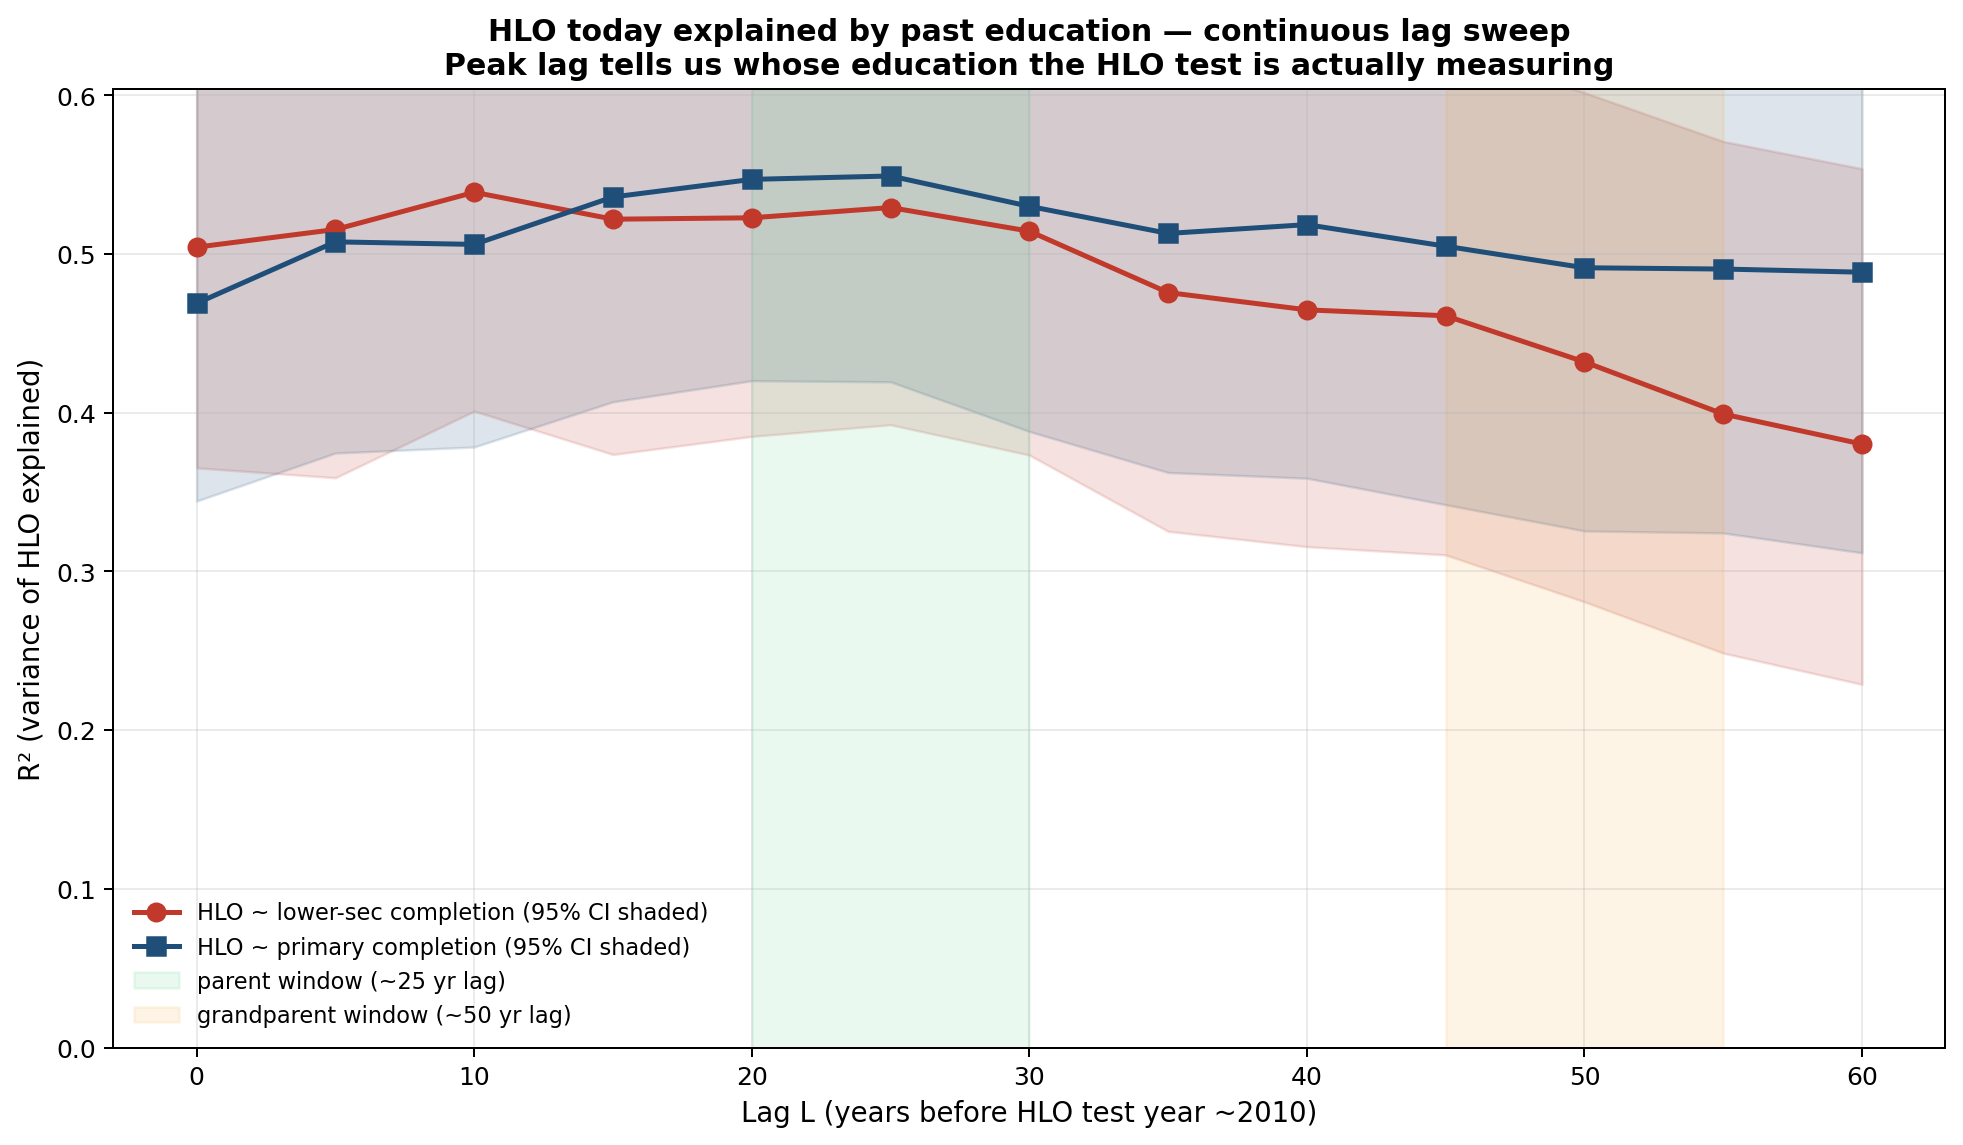
\includegraphics[width=0.95\linewidth]{figures/hlo_vs_education_lag_sweep.png}
\caption[HLO secondary today versus WCDE completion across a lag sweep]{HLO secondary today regressed on WCDE completion at year
$2010 - L$, for $L = 0, 5, \ldots, 60$. Shaded bands are 95\%
country-resample bootstrap CIs (2{,}000 draws). The curve is broad
and flat across the full lag sweep; primary completion at lag 60
(1950, more than two generations back) explains R² $=$ 0.489 of
today's variance, against R² $=$ 0.469 for the freshly-completed
cohort's primary. The freshly-completed cohort is a worse predictor
than either parental or grandparental-generation completion.
\emph{(Source: Angrist et al.\ 2021 for HLO, WCDE v3 for completion.)}}\label{fig:lag-sweep}
\end{figure}

The direct test on the parental window: HLO secondary today
regressed on lower-secondary completion in 1990 (the parent cohort's
20--24 education) gives R² $=$ 0.523, $\beta = +1.94$ HLO points
per percentage point, $t = 9.1$, correlation $0.72$, on 77 countries
with USSR excluded. Fifty-two percent of cross-country
variance in Hanushek's cognitive-skills measure is the paper's
quantity measure, lagged one generation. The residual variance is
what school systems add \emph{above} the home-niche baseline: China ($+111$ points),
Viet Nam ($+111$), Singapore ($+93$), Portugal ($+76$), Japan,
Finland, Korea --- East Asian education reforms and select rich
systems do deliver real additional rungs above what the parental
generation transmitted. The negative residuals --- South Africa
($-116$), Ghana ($-108$), Albania ($-86$), Montenegro ($-72$) ---
mark school systems that undershoot the parental baseline, a
credential-inflation diagnostic independent of the Soviet case.

HLO is not a snapshot of current school quality. It is a
multi-generational education stock measured at the cohort that sat
the test. The mechanism predicts this directly: each generation's
schooling is encoded in the parents' inventory of installed rungs,
which becomes the home niche the next generation absorbs the school
niche through
(Chapter~\ref{generational-transmission-and-state}). Compounding across
generations produces the variance HLO measures: the one-generation link is
direct and strong here, the deeper generational depth is carried by the
panel's grandparent channel (Section~\ref{the-grandparent-channel}), and the
lag sweep shows only that the cross-section is consistent with reach beyond a
single generation. Contemporary schools add the visible residual. The cross-country institutional-quality
confound that the test-score literature has long worried about
(``these countries are just better at everything'') is addressed by
the panel's country fixed effects
(Chapter~\ref{the-panel}) and by the Korea/Philippines matched pair
(Section~\ref{korea-and-philippines}), which holds institutional
quality roughly constant and varies only the schooling regime,
alongside the wider natural experiments and country histories
(Chapters~\ref{natural-experiments}--\ref{country-histories}). The lag-sweep is itself cross-sectional --- HLO is
observed once per country, so the within-country fixed-effects
machinery that anchors the rest of this chapter does not apply
directly to it. It sits inside the surrounding identification
structure as a consistency check: the cross-section behaves the way
the panel's mechanism predicts. The causal weight is carried by the
panel and the matched-pair experiments; the lag sweep is the test of
whether HLO --- read across the right time horizon --- still tells
the same story.

The horse race Hanushek called for partitions as the mechanism
predicts: every outcome loads on the same lower-secondary completion,
each read forward at its own biological lag rather than on a separate
depth of schooling.
Section~\ref{the-generational-lag} reports the full
quantitative partition.

\subsection{The Panel Excludes the Republics By Construction}\label{exclusion-robustness}

The expansion-sample headline design already excludes the 15 USSR
republics by construction: their reported lower-secondary completion
sat above the 90\% ceiling by 1975, placing them outside the
active-transition window the regression covers. Re-running the
panel with the USSR republics flagged as excluded changes nothing
because they were never inside the sample: the parental-education
coefficient stays at $\beta=0.707$ ($n=945$, $144$ countries,
$R^2=0.561$); LE, TFR, and U5MR forward-prediction $R^2$s also
hold identically ($0.384$, $0.630$, $0.650$). The Goskomstat
reporting concern affects countries the expansion-window design
already screens out.

This is not survivorship under contamination. It is two independent
design choices pointing at the same set of countries. The
expansion-window screen is mechanism-driven: the panel covers
countries while the parental-to-child completion ratchet is still
operating (10\%--90\% lower-secondary in the cohort). The Soviet
republics fall outside that window for the same reason any saturated
system does. The reporting concern and the regression scope converge.

One sentence summarizes the chapter. My mechanism identifies which
Soviet numbers were not real; the panel's expansion-window screen,
designed on entirely separate grounds, excludes those same republics
from the headline regression. It is the kind of agreement between
two independent constructions that one does not get by accident.

\section{What Every Framework Was Reaching For}\label{what-every-framework-was-reaching-for}

% A-prefix group removed: colonial-test table now numbers continuously with body.
%


The argument stands on the preceding chapters; this chapter reads what the field had almost found, not for confirmation but for what every prior framework had been reaching toward.

Every framework in this chapter answers one question: what makes some nations develop and others not? It is an old question, and it has been answered before by the differences between peoples --- by race and civilisational rank in the nineteenth century, by culture and creed after Weber, by institutions and income in our own. Each answer was discredited by the next, and each failed the same way, because development is not a property some peoples have and others lack. It is what one universal inheritance --- the long childhood --- produces once it is loaded with literate cultural transmission; and the childhood is the same in every human population, loaded in some and not yet in others. What differs across the accounts below is never the people and never the childhood, only the loading: whether it happened, how deep, how fast, and whether it was real. The loading does not invent cooperation, nor the institutions built from it --- those are what our social inheritance has always built --- but it adds effects no pre-industrial empire ever produced, the fertility, survival, and longevity gains, and it changes the scale at which the institutions hold (Section~\ref{literate-ct}).

Two of the frameworks below --- Sen and Drèze (§\ref{sen-and-dreze-two-routings}) and Easterlin (§\ref{easterlins-question}) --- reach the loaded childhood from the other side; I complete them rather than rebut them.

\subsection{Smith and the Loaded Labour}\label{smith-and-the-loaded-labour}

Smith (1776) founded the modern account of wealth on specialisation, taking as given the loaded Scottish labour that Knox's parish schools had produced over the preceding century (Section~\ref{specialisation-requires-loaded-labour}). The founding error propagated through two distinct descendant lines. The wage-frame line --- Smith to Schultz to Becker (Section~\ref{human-capital-and-the-wage-frame}) --- prices the loaded labour rather than naming what loaded it. The capabilities frame --- Sen (Section~\ref{sen-and-dreze-two-routings}) --- enumerates what educated agency produces without specifying the categorical reorganisation that makes the agency possible. Both lines rest on the substrate; both omit it from their causal accounts.

Smith found the engine of wealth in self-interest twice: we owe our dinner to the baker's self-love, not his benevolence, and the merchant seeking only his own gain is led by an invisible hand to serve an end no part of his intention. But self-love is the one human constant --- it bought no dinner and served no public for the three hundred thousand years before schooling. What changed in his Scotland was the population, not the motive: eighty years of parish schooling had made strangers legible enough to weigh, price, contract, and credit one another (Section~\ref{specialisation-requires-loaded-labour}). His hand is invisible because no one moves it; the schooling was invisible because everyone did. He found two marvels in self-love and missed the one beneath both --- the loaded labour that was the only reason self-love had anything to coordinate.

The cost is not conceptual alone. Policy built on Smith tells countries to specialise into export markets to get rich. Korea did the opposite; Taiwan did the opposite; Bangladesh did the opposite. Each built the substrate first and the specialisation followed. The mechanism predicts this ordering; Smith's frame, taken as primary, reverses it.

\subsection{Human Capital and the Wage Frame}\label{human-capital-and-the-wage-frame}

Schultz (1961) and Becker (1964) founded the human capital school on the observation that education raises individual wage productivity and can be treated, economically, as an investment yielding private returns. The framework is the operating frame of labour economics and much of education policy. Measurement of the private return to individual schooling is well developed within it.

The mechanism is that, in the first-generation transition from illiterate to literate, the private labour-market return is the secondary channel. Education's primary effect during that transition is not on the newly-educated person's wages but on their children's lives --- through the cognitive and decision-making traits transmitted parent-to-child (Chapter~\ref{generational-transmission-and-state}). A mother's education shows up in her children's mortality, nutrition, and school completion at effect sizes that dwarf its effect on her own wages. The Gakidou et al.\ (2010) decomposition (Section~\ref{the-deaton-objection}) captures this at population scale during the developing-country transition window: a half-of-mortality-decline intergenerational effect, not a labour-market effect.

Human capital theory treats this downstream effect as an externality and sometimes adds it to private returns. The mechanism reverses the ordering for the transition itself. During the illiterate-to-literate crossing, a parent's effect on her children is primary; the private wage return on her own schooling is the smaller, more variable side channel. Every country whose population crossed the educational threshold received the developmental compounding, whether or not the policy frame named the mechanism correctly. Korea, Taiwan, and Cuba did it in one generation under singular priority; the others did it slower under competing priorities, but the channel ran the same way. Once a population is past the threshold and home niches are fully literate, the intergenerational effect compresses toward the ceiling and the wage return becomes the dominant marginal signal --- but by then the developmental work is done.

The framework's narrower consequence is a misdirection of measurement. Decades of Mincerian wage-return estimation now anchor the policy question of whether schooling is ``worth it'' in developing countries. The answer from wage data is contingent and often uncertain. The answer from intergenerational outcome data is uniform and large. The disagreement is a frame choice, not a measurement dispute.

Underneath the frame choice is a category error about what kind of thing education is. Human capital theory files it as an asset: a stock a person accumulates and owns, that earns a private return and passes down by ownership within a lineage. Everything the frame guards against follows from that filing --- that the schooling of the advantaged might merely track their resources, that its worth is whatever a wage can be made to reveal, that a poor population catches up only as fast as it can build the stock. But the developmental payload is not an asset. It is the content of the second inheritance system (Chapter~\ref{generational-transmission-and-state}), and that system was never gated on ownership or descent. A resource-gated asset could not be loaded into the children of the unschooled poor at all --- yet that is exactly what every working school system does, which is why the private wage return can stay small and uncertain while the intergenerational effect stays large and uniform. And an asset compounds slowly and dynastically, whereas the payload of an inheritance system spreads on a same-species channel in a single transmission cycle: the one-generation crossings of Korea, Taiwan, and Cuba are the signature of a payload crossing, not a stock accumulating. The discipline priced the payload as if it were capital, and then predicted the dynastic, gradual, resource-bound catch-up that the panel refuses to show.

Galor's Unified Growth Theory (2011) extends the human-capital frame to the aggregate transition: rising returns to skill trigger a quantity--quality switch in fertility, which produces sustained growth. The empirical signature is the same one I report --- TFR falls as education rises --- and the cross-country panel is consistent with both engines. The mechanisms are not interchangeable. UGT's engine is the wage-return signal; mine is the categorical reorganisation that the dependency window installs whether or not the wage signal is present. The country histories identify the channel. Korea under Park, Cuba under Castro, Bangladesh through the 1980s and 1990s, and Mao-era China all expanded mass schooling under regimes where market returns to skill were absent, distorted, or politically suppressed. State commitment, not wage signal, drove the loading in each case. The shared scatter plot is what the two engines agree on; the country histories are where they part.

Heckman (2006; Heckman \& Cunha 2007; Heckman \& Mosso 2014) is the
human-capital strand that has reached furthest toward the window.
The empirical claim --- that returns to investment in cognitive and
non-cognitive skills are highest in early childhood and compound
across the life cycle --- runs in the same direction as the
dependency-window argument: what is loaded in the juvenile window has
higher leverage than anything added later. The Perry Preschool and
Abecedarian follow-up data and the technology-of-skill-formation
framework are the rigorous individual-level version of part of the
population-scale claim I make. The distance is still a layer. Heckman
prices the skills installed in the window and pushes policy toward
earlier investment within a still-monetised return framework; the
mechanism here is that the window itself is a species-level fact,
that the categorical reorganisation it permits is not reducible to a
stock of priceable skills
(Section~\ref{categorical-brain-reorganisation}), and that the
developmental compounding runs through population-scale home-niche
routing rather than individual labour-market wages. The frames agree
on the policy implication for the early years; they disagree on what
the early years are doing, and on whose returns matter. The closer
alignment is with Easterlin
(Section~\ref{easterlins-question}) and Lutz \& Kebede (2018), which
this paper extends rather than displaces.

\subsection{Growth Theory and the Residual}\label{growth-theory-and-the-residual}

Solow (1956) founded modern growth accounting on a production function with capital, labour, and exogenous technology. The Solow residual --- the share of cross-country output growth unexplained by measured capital and labour --- is what the substrate looks like when you refuse to name it. Treating labour as an undifferentiated input assigns the unexplained share to ``technology'', but technology is not a free input falling on the economy from outside it. Educated populations produce technology, and educated populations are what absorb it. The residual hides the substrate at the creation end and at the adoption end at once. Without categorical literacy at scale, the residual is small or zero --- the pre-1800 record is the test. With it, the residual is the population's own output measured as if it came from nowhere.

Romer (1986, 1990) closed Solow's gap by treating technology as endogenous --- produced by R\&D spending inside the economy and non-rival in use. The move from exogenous to endogenous technology is a real advance, and the post-Romer growth literature is built on it. The engine still has no name. Ideas are produced by educated populations and spread among educated populations; the R\&D-spending variable Romer measures is the budget line through which a country routes a small fraction of an already-educated workforce into formal research. The substrate is what makes the routing possible at both ends --- researchers who can produce the ideas, and a downstream population that can absorb and apply them. Solow says technology is exogenous and unmeasured; Romer says technology is endogenous and measurable as R\&D; neither names the educated population that produces ideas at the source and adopts them at the destination.

Mankiw--Romer--Weil (1992)\footnote{David Romer; not the Paul Romer of the preceding paragraph.} augmented Solow's production function with human capital as a stock variable --- secondary enrolment of the working-age population --- and reported that the augmented model explains most of cross-country income variation. This is the closest the growth literature comes to naming the substrate, and it is the most-cited move in the discipline. It still does not name it. The stock is priced as a labour-input multiplier, schoolyears monetised through wages, which is the same engine UGT runs at the aggregate scale (Section~\ref{human-capital-and-the-wage-frame}). What MRW measures is the cumulative output of past schooling cohorts entering the labour market; what it does not measure is the dependency-window loading that put them there, the home niche that gates absorption, or the household decisions through which the stock's children produce the next cohort's outcomes. MRW prices what was loaded without naming what loaded it.

The arc from Solow through Romer to Mankiw--Romer--Weil is the discipline working at the wrong layer. The residual was never a measurement gap to be closed by adding R\&D or human capital as a stock; it was the trace of the substrate --- the educated population, registered in the data as a number with no obvious owner. The growth literature has been pricing what loaded the labour without naming what loaded it --- the same error Smith made (Section~\ref{smith-and-the-loaded-labour}), with mathematics added.

\subsection{Diamond and the Geographic Objection}\label{diamond-geographic-objection}

Diamond (1997) argues that geography --- the distribution of domesticable plants and animals, the east--west axis of Eurasia, the biogeographic inheritance of different continents --- explains the differential trajectory of human populations. The argument is historical and long-run; it is not primarily about the post-1950 development window the panel here covers. On its own horizon it is largely right. Populations that inherited rich substrates of domesticable species developed settled agriculture earlier, accumulated food surpluses, and built the first stratified societies on those surpluses.

What the geographic frame cannot do is substitute for the mechanism that translates the geographic inheritance into developmental outcomes at any given point in time. The substrate for which environments could be rebuilt --- the long juvenile dependency (Chapter~\ref{longest-juvenile-dependency}) and the cultural-transmission channel (Chapter~\ref{cultural-transmission}) --- has geographic prerequisites in its deep evolutionary history; that is not in dispute. What geography does not do is fix the moment at which a particular country decides whether to put children in classrooms, and at what pace.

The Korea/Philippines pairing carries the point at country level (§\ref{korea-and-philippines}): the Philippines ahead in 1950 on income per capita, on lower-secondary completion, and on colonial educational inheritance, and behind by 2000 on every development outcome. Geography did not flip the rank order; the educational regime did. The panel is full of such pairings.

Geography is the substrate on which the mechanism runs. It is not the mechanism. The confusion of the two levels is the same shape as Smith's confusion of specialisation with the loaded labour specialisation operates on.

\subsection{Sen and Drèze: Two Routings, One Mechanism}\label{sen-and-dreze-two-routings}

Sen (1999) and Drèze and Sen (1989) are the closest frameworks to the one I make. The distance is a single step: what generates the capabilities.

Sen argues that development is what people are able to do and to be, not what they earn. The list of capabilities --- to live a long life, to be literate, to participate politically --- is the right list, and measuring development in those terms is a correction of the GDP-primary frame. Drèze and Sen's claim that democracy with a free press prevents famine is a genuinely novel observation largely right on its own evidence.

What the frame underdetermines is the mechanism that produces the capabilities in the first place. Sen treats them as parallel expressions of human freedom --- coequal axes of wellbeing. The mechanism is that they are serial consequences of a single substrate. Educated cognition makes categorical choice possible (Chapter~\ref{education-as-payload}); categorical choice, applied at the household scale, produces the fertility transition, the mortality transition, and the political capacity that the capabilities list comprises. The list is the output of one mechanism, not a set of independent dimensions: educated cognition is not one capability on the list, but the capability to have capabilities.

The distinction matters most for the growth-mediated / support-led dichotomy. Drèze and Sen describe two routings of fiscal resources --- through market growth or through state service provision --- and identify democratic accountability as the feature that determines which populations receive which routing. Both routings, in their own data, produce development only where they reach an educated population. The China case (Section~\ref{china}), matched on mean years of schooling to the fastest movers in the support-led list, shows the residual attributed to ``support-led'' routing is education itself. Costa Rica was treated as a similar exception in the 1980s --- high life expectancy at low income, attributed to its universal-coverage health system --- but South Korea, which began that period at much lower income and lower life expectancy than Costa Rica, ran the substrate path harder and now has substantially deeper schooling; by the 2010s Korea overtook Costa Rica on life expectancy and continues to climb past it. The residual that distinguished Costa Rica was real but bounded; substrate growth eventually overtook it. Bihar and Kerala (Section~\ref{the-famine-test}), under one constitution and one national press, isolate the mechanism: where most households are educated, the community-level shield forms and famine does not arrive; where most households are not, the shield does not form and press coverage alone does not substitute.

The frame is the same frame, read one layer deeper. The fiscal routing is how resources arrive; the educated household is where they become the capability.

\subsection{Schooling and Learning}\label{schooling-and-learning}

Pritchett (2013) argues that schooling in many developing countries fails to produce learning: children sit in classrooms for years and finish unable to read, do arithmetic, or reason at grade level. The measurement is accurate; cross-national assessments confirm wide gaps between years of schooling and measured proficiency. The policy consequence Pritchett draws is that schooling quality, not schooling coverage, is the development variable.

The biology disagrees on the mechanism. Duration of exposure to the categorical, symbolically organised environment of formal schooling is what restructures cognition (Chapter~\ref{education-as-payload}). Test scores measure one narrow output of that restructuring at a particular moment in a child's life; they do not capture the restructuring that has already taken place. The restructuring itself is observable at the neural level, not inferred from behaviour (Section~\ref{categorical-brain-reorganisation}). These structural changes persist whether or not the curricular content on which they were installed is retained for a particular test. The panel is the population-scale evidence: within countries, as lower-secondary completion expands, fertility, under-five mortality, and life expectancy all move (Chapter~\ref{the-panel}). The cross-country horse race in which cognitive test scores out-predict completion (Table~\ref{tab:composition}) is not the counterexample it appears to be --- I show in Section~\ref{hanushek-reconciliation} that those same test scores are themselves predicted by the previous generation's years in school, so the cognitive quality Pritchett would substitute for coverage is in large part coverage already compounded one generation back. A child with nine years of low-quality schooling in rural Bangladesh reaches adulthood with a different cognitive architecture than a child with three years of high-quality schooling, and the household-scale behaviour that follows reflects the first child's architecture, not the second's score.

The schooling-without-learning frame is a level-of-measurement mistake. Learning is measured in content absorbed; the mechanism is that schooling's primary effect is categorical --- the brain's reorganisation toward symbolic and propositional thought --- and that content is the disposable vehicle on which duration rides (Section~\ref{duration-over-fidelity}). This is a strong claim, and it implies that the curriculum wars that dominate education policy are second-order. The historical record is the test.

Four successful educational expansions ran through ostensibly different content regimes and converged on the same outcome. The convergence itself is the point: the wrapper at the entry of each expansion shed toward secular categorical instruction, because the categorical reorganisation schooling installs (Section~\ref{categorical-brain-reorganisation}) does not require doctrine and the doctrine drops away.

Scotland after 1560 taught scripture. Knox's parish schools were designed to make every child capable of reading the Bible, because Protestant salvation required direct textual access and Knox did not trust intermediaries. The content was religious at the entry. Over the following two centuries the curriculum secularised --- arithmetic, geography, classical letters, and eventually the natural sciences entered the parish schoolhouse, and the scripture share fell. The categorical instruction that produced the highest parish-level literacy in Europe by Smith's lifetime --- the loaded labour Smith observed in the pin factory (Section~\ref{smith-and-the-loaded-labour}) --- was secular by the time it scaled. Scripture was the starter; secular categorical schooling was what it became.

France under the Ferry Laws (1881--1882) taught secular classical literature, republican history, and a standardised national curriculum designed specifically to displace religious instruction. France entered where Scotland arrived. The effect was mass literacy across the French population, independent of whether the pupil retained the Latin declensions or the list of French kings.

Cuba in 1961 taught literacy through revolutionary primers --- Castro's speeches, political slogans, revolutionary narrative. The doctrine was the surface. The teaching underneath was secular: phonemes, letters, reading sentences, doing arithmetic. By the time Cuba's literacy brigades had completed the campaign, the population had been categorically reorganised through secular instruction wrapped in revolutionary content, and the subsequent schooling system that built on it taught the same secular categorical material every other modernising schooling system teaches. Cuba's development trajectory --- fertility transition, mortality transition, life expectancy tracking high-income countries despite low GDP (Section~\ref{four-further-cases}) --- followed.

Bangladesh expanded schooling through the 1980s and 1990s with a secular curriculum that, by Pritchett's own measurement, produced substantial learning deficits. The content was weak in exactly the sense that motivates the schooling-without-learning critique. The effect was a fertility transition and a mortality transition that place Bangladesh among the paper's policy over-performers (Section~\ref{universality-across-subsamples}).

Scripture-then-secular, secular-by-design, revolutionary-wrapper-on-secular, weak-modern-secular. Four entry conditions, one trajectory: secular categorical instruction at scale. The wrappers selected who built the schools and how the expansion was sold; they did not select what the schools did to the children inside them. Duration of exposure to secular categorical instruction selected whether the cognitive reorganisation happened at all. The curriculum wars mistake the wrapper for the payload.

Coverage is the primary policy variable. Quality is a second-order adjustment on top of coverage, not a substitute for it.

\subsection{The Deaton Objection}\label{the-deaton-objection}

Deaton (2013) attributes the post-1950 mortality decline to global health technology diffusion largely independent of education. The argument is: vaccines, antibiotics, oral rehydration therapy, and safe-water knowledge are cheap, globally available, and easily applied; once the technology is invented, populations benefit without needing to understand the science behind it; the curve rises because the technology spreads.

The distribution of outcomes does not agree. Vaccines have been globally available since the 1960s; under-five mortality fell sharply in some populations and barely moved in others over the same decades. The technology diffused; the outcomes did not, uniformly. Between the existence of a vaccine and a vaccinated child sits a household decision --- to locate the clinic, to trust the schedule, to complete the series, to act on subsequent infection warning signs. Each of those is a small act of categorical reasoning on a medical claim. Educated mothers make those decisions reliably; uneducated mothers make them variably. Gakidou et al.\ (2010), decomposing the global mortality decline, attributed roughly half of the post-1970 reduction in under-five mortality to gains in women's education.

The panel confirms the channel: if technology operated independently of education, residualised GDP would retain predictive power once education is partialled out; it does not (Section~\ref{gdp-has-no-independent-effect}).

The objection also has a date, and the date refuses it. I run the same
within-country regression of cohort education on later life expectancy
and child mortality on the only populations whose vital registration
reaches the nineteenth century: the early-industrialising states whose
mortality the Human Mortality Database records and whose cohort
education the WCDE series carries back to 1870, restricted to outcomes
before 1945 --- before antibiotics or mass childhood vaccination
existed anywhere in the sample. The education coefficient is already
present and already signed the way the modern panel signs it: life
expectancy $+0.404$ (cluster SE $0.095$), under-five mortality
$-2.977$ (cluster SE $0.636$). Fit that pre-antibiotic era alone and
ask it to predict mortality from 1960 forward --- the decades Deaton
attributes to technology --- and the same coefficients carry across the
regime break ($+0.566$ and $-3.464$). The relationship that lowered
child mortality before the antibiotic is the relationship that lowers
it after.

That window is not pre-medicine; it is the sanitation and germ-theory
revolution itself --- clean water, sewers, the science of Snow, Koch,
and Pasteur. But that revolution is the ratchet running
(Section~\ref{the-human-ratchet}), not a wave arriving from outside it:
its science came from the thin elite layer Mokyr names the Republic of
Letters, which grows out of the loaded mass beneath it
(Section~\ref{innovation-and-the-cultural-substrate}); its waterworks
were built by educated states; and its hygiene was adopted household by
household by populations already literate enough to act on a pathogen
they could not see. Education produced the technology at one end and
absorbed it at the other. Deaton's diffusion has no exogenous end: both
ends are the educated population.

The technology is necessary. It is not sufficient. The mechanism that converts the technology into outcomes is the educated household, one child at a time, and the community-level threshold at which that conversion becomes routine.

\subsection{The Methodological Frontier and Its Limits}\label{methodological-frontier}

Two methodological waves have organised the discipline's empirical
frontier for the past three decades. The credibility revolution
(Angrist, Card, and Imbens --- instrumental variables, regression
discontinuity, and difference-in-differences) and the randomised-trial
movement in development economics (Banerjee, Duflo, and Kremer ---
field experiments on poverty alleviation). Both produce
rigorous local effects of marginal interventions inside operating
systems. Neither reaches the channel I identify, and the
reasons are methodological in the strict sense.

The credibility-revolution toolkit estimates causal effects of small
treatments by exploiting natural variation that approximates random
assignment. The country histories the paper rests on
(Chapter~\ref{country-histories}) and the matched-pair natural
experiments (Chapter~\ref{natural-experiments}) are clean
comparisons of exactly the kind the credibility revolution
methodology aspires to. What the discipline's headline applications
of these methods have not done is converge on the channel as the
developmental cause, because the methods have been pointed at
marginal questions inside already-loaded systems --- the wage return
to one extra year of schooling, the test-score effect of class size,
the labour-supply response to a minimum-wage change. Each finding is
rigorous; collectively they accumulate without converging on the
channel, which is not a marginal question.

The randomised-trial methodology runs small experiments inside
operating educational systems: deworming, conditional cash transfers,
teacher incentives, textbook delivery. These produce defensible local
effects on the margin of an already-loaded system. They cannot run
a population-scale channel-loading experiment because no IRB will
randomise 50 million children to twenty years of no schooling. History
ran those experiments.

Korea and the Philippines began 1950 with comparable colonial
education bases --- the Philippines if anything ahead, on
lower-secondary completion and per-capita income alike
(Section~\ref{korea-and-philippines}); political accident assigned one
to singular educational priority and the other to competing
priorities; one generation later the developmental trajectories had
diverged completely.
North Korea and South Korea began 1953 as the same population on
either side of a frontline; the channel diverged; the outcomes
diverged. Cuba ran a literacy campaign in 1961 that loaded the
population in eighteen months and crossed the development threshold by
1974. Cambodia's educated cohort was destroyed in four years and the
developmental trajectory tracked the cohort's recovery rather than
income's. China after 1949 and Niger after 1960 began as comparably
impoverished, comparably illiterate states; one founded itself on
mass-education commitment and the other did not; seventy years of
compounding policy is the experiment.

These are natural experiments at the right scale --- not randomised, but with the treatment assigned independently of the outcome, which is what the inference requires. The treatment
is political commitment to mass education, assigned by historical
accident with respect to outcome. The control is the country that did
not get the treatment. The outcome is observable a generation later.

The hollow-education case (Chapter~\ref{hollow-education}) completes
the design. The Soviet republics carried reported lower-secondary
completion among the highest in the world over a channel that was
hollow; in the language of randomised trials, this is a
manipulation-check failure --- the treatment administratively imposed
without actually loading the variable the theory claims is causal, and
the outcome does not follow. The channel is what matters, not the
schooling reported on paper.

The credibility-revolution and field-experiment methodologies are
appropriate for the questions their applications address: marginal
effects of marginal interventions inside operating systems. Applied to the
question of why populations develop, the methodology cannot reach the
mechanism because the mechanism does not operate at the margin. It is
the channel itself. Borrowing that toolkit's vocabulary to defend the
finding would borrow the yardstick those tools were calibrated against,
and the channel is not on that yardstick. Evolutionary biology, in the
200 years since Wallace,
has established the mechanism --- drawing on comparative primatology,
ethnography, developmental psychology, archaeology, life-history
theory, and the evolutionary anthropology that synthesises them.
Those methods have produced a settled picture of what the human
species is. Development economics has produced a
sequence of frameworks --- Big Push, structural adjustment,
institutions, randomised intervention --- that replace rather than
extend each other. One field has named the underlying mechanism;
the other has measured its outcomes without naming what produces them.

The asymmetry has a cause, and it is not the diligence of either
field. Economics begins only when the childhood is already finished
--- loaded or not --- and takes its output as the primitive:
preferences, the human-capital stock, institutions, all entered as
givens the apparatus never watches form. Whether that childhood was
loaded or left empty is the one thing it cannot see, because it reads
the finished output the same way on either side. And everything it
measures is second-order to that childhood. Income, institutions,
markets, regulations are not the cause of development but the
operations of a population the loading already produced --- the
surplus an educated people generate, the structures they hold
(Section~\ref{the-institutional-challenge}), the exchange they
coordinate, the rules they can write and enforce. Income itself, the
quantity the discipline reaches for, sits inside that second-order
layer (Section~\ref{gdp-has-no-independent-effect}). Biology measures the
first-order term directly: the organism itself, in counts that hold
for the species (Section~\ref{what-the-panel-supports}). A field that
can reach only the second-order layer can price what the cause
produced; it cannot find the cause.

My natural experiments deliver the population-scale
identification the field's methodology aspires to and cannot run. Where the discipline has
read those experiments as ``case studies'' to be supplemented by
something more rigorous, I read them as the rigorous part.
The regressions are the supplement.

\subsection{The Institutional Challenge}\label{the-institutional-challenge}

Acemoglu and Robinson (2012) argue that institutions --- inclusive versus extractive --- are the primary determinant of long-run development. The question is which way the causal arrow runs.

I claim the arrow is asymmetric: education builds institutions, but institutional quality does not measurably accelerate the next generation's schooling. The forward arrow is real; the back arrow is near-zero in the panel.

Institutions act on the adults a country has. Schools act on the children it will have. The window for arranging humans is open continuously; the window for making them is fixed by biology and closes around eighteen. A generation spent reforming institutions optimises the arrangement of an unchanged input. A generation spent schooling the children changes the input itself, and the next generation's institutions are built by different humans. The asymmetry is general: education runs at the speed of demographic metabolism (Lutz 2013); every other policy lever runs at policy speed (Section~\ref{education-as-limiting-factor}).

Institutions are built by educated populations. The civil servants, judges, journalists, health workers, and administrators who constitute institutional capacity are the educated cohort. Without the underlying educated population, institutional reform produces forms without function. Controlling for institutions is controlling for a product of education.

An institution is not a thing a country has; it is an equilibrium it holds against decay. The people who run any institution act in their own interest, and so do the people shut out of it --- that is the baseline, not a flaw: incumbents capture it for rent, challengers tear it down to raise their own on the same terms. Every empire that rose had institutions adequate to its rising, and every one of them rotted, because the resting direction of an institution left to its own incumbents is toward extraction. So the presence of good institutions cannot be what explains development --- good institutions are read off success after the fact, and they do not stay good. What holds the equilibrium against the rot is continuous pressure from below, and only an educated population can sustain it: a population that can read, coordinate as strangers at scale, monitor the institution, and make itself too costly to ignore. The check that matters sits in the population, which renews every generation, not in the elite, whose incentives are the same in every generation. Reform from the top rearranges the adults a country already has and reverts when they do; schooling changes who the next generation is. Institutions are reasonable now, where no empire's stayed reasonable before, not because the people running them became virtuous but because a literate population forces them to work.

This is where I part from the institutional account at the root. Acquiring institutions was never the hard part. We are a shared-intentionality species (Tomasello 2014): cooperation, and the building of institutions out of it, is our default --- not a late achievement, but the baseline. The small ancestral band had institutions; every human group builds them. So the question is never how a people comes to \emph{have} an institution. It is whether, at the scale of millions, the institution can be \emph{held} --- and holding is a matter of force, not virtue. The costliness that forces an institution to work is not a special property of institutions; it is the whole of what any recognition rests on. A rival honours your claim only while crossing you costs more than honouring it. Property, the vote, the right not to be starved so that revenue can be collected --- each is a recognition extended exactly as far as its denial can be made expensive, and no further. An institution is the durable shape that balance of force settles into, mistaken after the fact for the source of the recognition it only records. What the evolved inheritance cannot supply is the holding at population scale. Cooperation is destroyed by the free-rider --- the member who takes the collective good and returns nothing --- and the only thing that suppresses him is being seen: the band caught him by sight, the cultural group by reputation, and both detectors go blind at the scale of millions of strangers (Tomasello 2016). The incumbent who captures the institution for rent is that free-rider at the radius where sight and reputation no longer reach, and what restores the cost on him is a population literate enough to see the capture at a distance. A crowd is not strength. A population that can read, coordinate as strangers, monitor, and withhold in concert is --- and mass literacy is the one renewable source of it.

Seen this way, the engine the institutional account proposes --- the virtuous circle, in which inclusive institutions widen the franchise and spread secure property rights of their own momentum --- is a balance of force misread as a property of the institution. Post-revolution England is held up as the birthplace of inclusive institutions --- but inclusive for whom? About 400{,}000 men could vote before the Reform Act of 1832; after the celebrated extensions of 1832, 1867, and 1884, roughly 40\% of adult men still could not, and no woman voted on equal terms until 1928. The same Parliament, in those same decades, ran the largest extractive machine in history: as many as ten million dead in the Bengal famine of 1770 under Company rule, one million dead inside the United Kingdom itself in the Irish famine of the 1840s, three million in Bengal again in 1943. The franchise extensions are read as the circle improving itself; they are nothing of the kind. Each is a bloc --- workers, tenants, women --- grown literate and coordinated enough to make its exclusion cost more than its admission. Nothing in the institution reached out to include them; they forced the door. Property tells the same story in its hardest form, because property is zero-sum where the vote is not: securing the landlord's title \emph{was} extinguishing the commoner's customary right, and the Company's secure claim on Bengal's revenue \emph{was} the famine. The right and the expropriation are one act seen from two sides of an edge, and the edge is who could make a claim expensive to deny --- the propertied man who could organise and vote on the inside, the Irish tenant and the Bengali peasant and the unenfranchised on the outside, at the same time, under the same rules. Where a population was kept illiterate by design --- the colonies --- it could generate no counter-pressure, and extraction ran unopposed through the same inclusive Parliament. ``Inclusive'' is not a property of an institution; it names who currently has the educated strength to stand inside the radius. The boundary of inclusion is the boundary of educated pressure (Section~\ref{from-action-to-talk-how-education-reaches-beyond-the-household}); the same scaled coordination that pulls the metropolitan worker inside extracts the colony (Chapter~\ref{the-dark-parallel}).

Institutions are therefore not a parallel cause. The developmental variable was never whether a country has institutions but whether, at the scale of millions, they hold and include rather than rot and extract; and that is set by the educated population beneath them. A court, a ministry, a bank, a registry is a structure for coordinating non-kin at a scale the band never reached, held by written rule and symbolic role rather than by kinship and line of sight. It is not that stranger-cooperation is absent from our inheritance --- it is that the inheritance enforces it only at band scale, and the apparatus that carries it to the scale of millions, the writing and the registry and the law and the literate population that can wield and read them, is what literate CT supplies (Section~\ref{literate-ct}). Agriculture built large polities before that flip --- on a literate elite over an illiterate-CT population --- and that complexity rose and then collapsed (Section~\ref{literate-ct}); only the flip to a whole literate population makes the scaled coordination hold. The scale an institution can reach is bottlenecked by the population's literacy, not the reverse. The capacity is the point, not the virtue: the same scaled coordination that builds a public-distribution system builds a war machine (Chapter~\ref{the-dark-parallel}).

Country fixed effects absorb time-invariant institutional characteristics. Time-varying institutional change is itself driven by education. Qatar (\$69,000 per capita, stable institutions by standard measures) delivered 3.1 percentage points below its generational education baseline in 2015. The institutions were present; the educational commitment was not; the development did not compound. The Philippines (Section~\ref{korea-and-philippines}) confirms the same point from the opposite direction: equivalent initial institutions, slower education, slower convergence. The same contrast appears within a single country: India's southern states and its northern BIMARU states sit under one set of national institutions, and their development still sorts by how much schooling each reached (Section~\ref{kerala}).

India has had democratic institutions, an independent judiciary, and a free press since 1947. China had none. China expanded lower secondary completion from 10\% to 75\% in 40 years (1950--1990) at 1.6 pp/yr --- under Mao, the Cultural Revolution, and the Great Leap Forward. India expanded from 10\% to 37\% in the same 40 years at 0.7 pp/yr --- with every institutional advantage the literature claims to matter. India's institutions did not accelerate education; China's absence of them did not prevent it. Among countries in the active-transition window (lower-secondary completion 10--90\% at decade start), the mean expansion rate peaked at 1.52 pp/yr in the 1960s --- before most postcolonial institution-building --- and fell to a trough of 0.74 in the 1990s, when the inclusive-institutions consensus was at its strongest. The series rebounded to 1.29 in the 2010s. Speed and institutional maturation do not co-move; in this panel they run counter.

Autocracy does not predict education speed. Merging Polity5 time-varying regime scores with the WCDE completion data (160 countries, 1950--2020, lagged 20 years to match the regime that made the schooling decision), polity2 explains less than 0.7\% of the variance in education gain rates --- the same null holds at 0-year and 15-year lags. Democracies are slightly faster on average: 10.3 pp/decade against 8.1 for autocracies at the 20-year lag.

What autocracy produces is not speed but \emph{variance}: 74\% of autocratic countries fall below the democratic median gain rate, but the fat right tail includes Korea and Cuba. Autocracies populate both the fastest and the slowest education trajectories in the dataset. Among 50 countries that transitioned, 30 were faster under democracy (paired mean $= +0.6$ pp/decade, $p = 0.57$).

Regime type is a variance amplifier, not a cause. The decision variable is education policy (Section~\ref{the-decision}), and it is orthogonal to regime type.

The colonial instrumental-variable contest (Section~\ref{the-colonial-test}) makes the same point from the institutional literature's own preferred instrument and its own 64-country base sample: education and AJR's expropriation measure are near-collinear ($r=0.62$) and explain near-identical shares of current GDP, because they share one colonial-era upstream cause. I read that cause as educational, the literature as institutional; the structural test follows in Table~\ref{tab:a6}.

This is not a heterodox reading. Glaeser, La Porta, López-de-Silanes \& Shleifer (2004) reached it from inside the institutional literature's own tools: the standard institutions measures are themselves outcomes, not primitives; the settler-mortality instrument predicts human capital at least as readily as it predicts institutions; and the dictatorships that grew --- Korea, Taiwan, China --- did so by accumulating schooling under exactly the institutions the account calls extractive. They argued it on growth and the cross-section. I argue it on the full panel, and on the outcomes growth does not reach --- fertility, life expectancy, child survival --- with the window mechanism beneath it and the back-arrow null behind it.

\refstepcounter{table}\label{tab:a6}\addcontentsline{lot}{table}{\protect\numberline{\thetable}Colonial education vs.\ AJR's avexpr as predictors of current GDP}Table~\thetable: Colonial education vs.~AJR's avexpr as predictors of current GDP.

\begin{longtable}[]{@{}lr@{}}
\toprule
Predictor & R$^2$ (log GDP 2020) \\
\midrule
\endhead
Education at independence (1950 lower sec) & 0.518 \\
AJR \emph{avexpr} (institutions, 1985--95) & 0.525 \\
AJR settler mortality (\emph{logem4}) & 0.544 \\
\bottomrule
\end{longtable}\addtocounter{table}{-1}% undo longtable's auto-step (we use manual \refstepcounter for labels)

\begin{minipage}{\dimexpr\textwidth-2em}
\scriptsize
\textbf{Notes:} AJR's base sample (n=61 with all data after
WCDE/WB merge). Education and AJR's avexpr explain near-identical
shares of log GDP variance because they share the same colonial-era
upstream cause. Education at WCDE v3, GDP at World Bank WDI (constant
2015 USD), avexpr and logem4 from AJR (2001) replication archive.
\end{minipage}

\subsection{Innovation and the Cultural Substrate}\label{innovation-and-the-cultural-substrate}

Aghion and Howitt (1992) is the Schumpeterian extension of Romer --- innovation as serial creative destruction, with the same R\&D-driven engine and the same substrate gap (Section~\ref{growth-theory-and-the-residual}). Mokyr is the harder target, because he reaches further than any major economist toward a cognitive-cultural substrate.

Mokyr (1990, 2002, 2009, 2016) argues that the Industrial Revolution was driven by a cultural substrate: the Republic of Letters, the rise of contestable beliefs, the seventeenth-century turn toward useful knowledge, and the Enlightenment's institutionalisation of open scientific inquiry. The argument has the right shape. A cognitive-cultural state of a population produces sustained technological growth; the state is historically specific and politically contingent; without it, the same material conditions produce no industrial transition. Mokyr is the only major economist who has reached for the substrate as a causal frame --- not merely priced it as a stock, the way MRW does --- and the substrate he names is real.

Mokyr's framework distinguishes propositional knowledge (the elite epistemic shift) from prescriptive knowledge (artisan technique and useful know-how), and treats the connecting institutions --- mechanics' institutes, learned societies --- as the transmission belt between them. The causal weight nonetheless runs from the elite tier down: contestable beliefs in the Republic of Letters change the norms, and the norms propagate to artisans through institutional channels.

The frame names the wrong layer. The Republic of Letters played in salons, journals, and learned societies of perhaps a few thousand correspondents across Europe; the Industrial Revolution was assembled by hundreds of thousands of parish-school graduates working looms, lathes, and forges in workshops across Britain. Knox's parish schools (Section~\ref{specialisation-requires-loaded-labour}) produced the loaded labour that made Smith's pin factory possible a century before Mokyr's Enlightenment thinkers met. Mokyr describes the elite layer; the population layer is in the data underneath his account, not central to it.

The two layers are not parallel; the elite rises from the population substrate. The engineers, philosophers, and experimentalists Mokyr describes are a small fraction --- a hundredth, a thousandth --- of a loaded population. Indian and Chinese brains in 1900 were no less capable than the engineers from those countries now filling Silicon Valley; what changed is that both populations were loaded through schooling. Take the loading away and the same brains do the work their forefathers did --- subsistence agriculture, the labour of the unloaded. Song China, Abbasid Baghdad, and Renaissance Italy produced elite cognitive cultures without industrial transitions because the elite was thin and the population beneath it was not loaded. The Chinese imperial examination system selected a few individuals from that population; it did not load it. The population substrate is the layer at which the post-1950 convergence runs (Chapters~\ref{the-prediction}--\ref{the-panel}), and at which the Industrial Revolution itself was assembled. Mokyr names the elite; I name the layer that grows it.

\subsection{Easterlin's Question}\label{easterlins-question}

Easterlin (1981) asked, and answered, the question I extend: \emph{Why isn't the whole world developed?} Lutz and Kebede (2018) extended that answer empirically; I extend both.

The question's persistence in the literature four decades after Easterlin asked it reveals what the discipline of development economics has done with the answer he gave. The frame that took hold instead was growth-first, with the claim that education would follow, adjusted to whichever framework was ascendant: human capital in the 1980s, institutions in the 2000s, schooling-versus-learning in the 2010s. None of those frames permits Easterlin's answer, because each subordinates education to something prior. The substrate-is-primary claim is what those frames cannot absorb.

The whole world is not yet developed because the substrate-level investment is generational, and because most countries, in most decades since 1950, did not make the singular-priority decision (Section~\ref{the-decision}). The countries that did --- Korea, Taiwan, Cuba --- compressed the transition to one generation. The rest proceed slower under competing-priority regimes. Easterlin asked the right question and gave the right answer; I add the biology beneath it, the empirics that confirm it, and the invisibility argument that explains why his answer did not take.

% closing brace of A-prefix group removed

\section{Why the Loading in Childhood Is Invisible}\label{why-the-loading-in-childhood-is-invisible}

Childhood is visible. The loading happening inside it is not.
Every framework in the previous chapter was reaching for this
cause and stopped a layer short of it
(Chapter~\ref{what-every-framework-was-reaching-for}); the
invisibility is the structural reason why. The capacity to rank education as fundamental
requires a cognitive frame that only education produces. I make
that invisibility precise here, and close by turning it on the
present synthesis.

\subsection{Education Leaves No Physical Signature}\label{education-leaves-no-physical-signature}

An educated person is physically indistinguishable from an uneducated
one. Same body, same biological drives, same appearance. Wealth builds
visible infrastructure; disease marks the body; education rewires
cognition and leaves no trace on the surface. The only observable signal
is behavioural change --- and the disciplines misread it. They see
smaller families and call it wealth flows, or contraceptive access, or
patriarchy relaxing, or telenovelas on television. They see longer
lives and call it health systems. They see rising productivity and
call it economic growth. Every discipline
theorises the downstream behaviour without tracing it back to the
cognitive reorganisation that produced it. Education has no physical
signature, so the signature it does leave --- changed decisions, across
every domain, for the rest of the person's life --- is assigned to
whatever domain notices it first.

The timescale compounds the invisibility. Education works through
demographic metabolism (Section~\ref{education-as-limiting-factor};
Lutz 2013): its effects appear as new cohorts replace older ones,
on horizons of twenty-eight years, not in the year-over-year cycles
that policy attention, news, and electoral politics are tuned to.
A signature too slow for a news cycle and too distributed for a
policy ledger is a signature easy to miss, even when its
accumulated mark is the largest in the developmental record.

\subsection{Invisible From Inside}\label{invisible-from-inside}

Educated people rank education as important --- one of many important
things, alongside health, nutrition, governance, and security. They
cannot categorise it as \emph{fundamental} because that would require
seeing their own cognition from outside. The act of ranking priorities
is itself an educated act; the cognitive architecture that assembles
competing inputs into a weighted comparison is the product of the
substrate I describe. The medium cannot be seen by those
thinking through it.

Pinker's (2018) \emph{Enlightenment Now} is a representative case.
Pinker attributes the post-1800 rise in life expectancy, literacy,
wealth, and peace to ``reason, science, humanism, and progress.'' The
rise itself was education. Literacy is education by definition.
Life expectancy, wealth, and peace are what educated populations
produce --- longer lives because educated adults care differently for
themselves and their children, material gain because educated labour
can be loaded with specialised skill, reduced violence because educated
populations have fewer children, releasing the demographic and
Malthusian pressure that drives conflict (Chapter~\ref{the-dark-parallel}). Reason, science, and humanism
are what schooling installs in the mind, the cognitive residue
of the same mechanism. Pinker has described education twice --- once
as outcome, once as mechanism --- without recognising that formal
schooling is the common cause of both sides. The book is a compendium
of the downstream outcomes of the mechanism in
Chapters~\ref{longest-juvenile-dependency}--\ref{education-as-payload}
without a chapter tracing them to schooling. A reader inside the
educated frame reads this as persuasive because the frame is what
produces the reading. From outside the frame, the chain is one step,
not two: mass schooling produced successive cohorts of educated adults,
and those cohorts produced the measurable gains Pinker documents.

Subjective wellbeing confirms the blindspot: across 159 countries,
self-reported happiness tracks income, not education --- people feel
richer, not more educated, so they attribute progress to
wealth. The signal
educated populations receive from their own lives is material
improvement, not cognitive transformation; the transformation is the
medium through which they perceive the improvement.

There is a structural reason the misattribution runs so reliably to
income. The convergence is the leaderless flock's turn of
Section~\ref{the-state-reach-not-mechanism} --- built from private
household decisions no one coordinates, each made for its own reasons.
With no leader and no movement for the eye to land on, the observer
credits the single thing that is visible and counted: the money. It is
invisible from inside not because it is hidden but because a shape no
one made looks like no one's doing.

\subsection{The Dilution Mechanism}\label{the-dilution-mechanism}

Education simultaneously widens who the educated person invests in
(literacy connects her to populations she has never met) and creates
surplus to invest (fewer children, healthier children, longer
productive life). The combination disperses investment across every
cause simultaneously: health, poverty, gender equality, climate,
governance, animal welfare, the arts. This is not a failure of
educated people; it is the structure of educated behaviour. The
educated adult, by the time she can evaluate priorities, has absorbed
the frame in which priorities are plural by default.

The result is a global development discipline that treats education
as one input among many. This is what the competing-priority regime
(\S\ref{the-state-reach-not-mechanism})
looks like at the intellectual level: the educated frame produces
dispersion as its native output, and the institutions built by
educated people inherit the dispersion. Education sits at number
four in the SDG framework not because the framers mis-specified, but
because the frame through which they specified is itself the output
of education operating at its widest radius.

The clearest contemporary demonstration of the dilution mechanism is
the United Nations Sustainable Development Goals (UN 2015). The SDG
framework was designed by the most credentialed development
institutions on earth, with full access to the evidence I
cite --- including Haq and Sen's own Human Development Index,
Easterlin's identification of mass schooling as the binding
constraint, and the income--health literature showing education
proxying through income. The result: SDG 4, Quality Education, listed
fourth among seventeen parallel goals --- alongside SDG 1 (No
Poverty), SDG 2 (Zero Hunger), SDG 3 (Good Health), SDG 5 (Gender
Equality), SDG 8 (Decent Work), and SDG 10 (Reduced Inequalities).
Every one of these is a downstream product of education.

Income is what educated populations generate
(Section~\ref{gdp-has-no-independent-effect}). Hunger is what educated
households escape --- not through provision but through the fertility
transition that releases resources per child, the planning horizon that
converts subsistence into surplus, and the household-level cognitive and
behavioural capacity that prevents food shocks from becoming famines.
19 of 21 post-1950 famines occurred where lower-secondary completion
was below 50\% (Section~\ref{the-famine-test}). Gender equality
is what the fertility transition produces first --- the shift from
biological fate to conscious reproductive choice that occurs at primary
education, before labour force participation, before political voice,
before any of the dimensions SDG 5 measures independently.

The SDG framework does not reflect ignorance of the evidence. It reflects the
mechanism: the educated people who designed it experienced income, food
security, health literacy, and institutional capacity as the normal
baseline from which you design frameworks --- not as products of
education that the uneducated world does not yet have. Education at
number four, competing for budget allocations against hunger programs
that feed children today, poverty interventions with visible short-term
outcomes, and health delivery systems that save lives this year, is not
an oversight. It is what the competing-priority regime looks like when
institutionalised at the global scale by people who cannot see they are
inside it.

\subsection{This Applies to This Paper}\label{this-applies-to-this-paper}

My argument applies to its own production, and to the
production of every argument, discovery, and specification in the
history of ideas. I received categorical literacy through
formal schooling. The biological components of the mechanism --- Konner
on juvenile dependency, Boyd and Richerson on cultural transmission,
Hawkes on post-reproductive lifespan, Dehaene on literacy's neural
reorganisation --- and the development components --- Haq, Sen,
Easterlin, Lutz and Kebede --- arrived through the same transmission
channel I describe. The synthesis is that channel operating on
itself: an instance of what educated minds do with accumulated payload,
no different in kind from any other output of the mechanism.

Every foundational specification is produced this way. Smith wrote from
within an educated Scotland whose parish schools had been building
literate labour for a century before him; he took the literate workforce
as given and theorised the division of labour it enabled. Wallace
wrote from the Malay Archipelago, having left formal schooling at
fourteen; he carried the accumulated tradition of Linnaean taxonomy,
Lyellian geology, and Malthusian population dynamics --- each diffused
to him through books and lower-tier British schooling rather than the
Edinburgh--Cambridge elite circuit (Wallace 1870). Darwin reached the
same synthesis independently because the tradition was ready. Shannon
wrote
from within the mathematical-engineering tradition of Nyquist, Hartley,
Wiener, and Turing. Mendeleev assembled Döbereiner, Newlands, and Meyer
into the periodic table; Meyer reached a parallel arrangement the same
year. In each case the specifier is a node in a transmission chain that
has reached the threshold where the chain's own mechanism can be
articulated from within.

Traditions specify their own mechanisms at readiness-moments. The
specific author is contingent; the readiness is not. Parallel synthesis
--- Leibniz and Newton, Wallace and Darwin, Meyer and Mendeleev --- is
the usual signature of a tradition arriving at its own self-description.
What matters is that the accumulated components reach the point where
synthesis becomes possible, not who performs the synthesis.

This closes the invisibility from inside the frame. The
capacity to see the mechanism from inside is produced by the mechanism
itself, operating across enough generations of accumulated knowledge
that the channel becomes describable in its own terms. Education is
invisible at shallow depths of accumulated understanding and specifiable
at sufficient ones. The present synthesis is the tradition Haq and Sen
opened in 1990, and the evolutionary biology beneath it, reaching
together the depth at which their shared operative channel can be named. The paper is the channel speaking about itself --- late,
contingent, and no more exterior to the phenomenon than any other
educated output ever has been. What separates this synthesis from competing ones is empirical survival across every line of evidence --- the deep-history mechanism, the natural experiments, the country histories, the panel, and the Soviet falsifier --- not its provenance.

\section{The Dark Parallel}\label{the-dark-parallel}

The positive case has been stated, defended, and shown to be invisible
even from inside: education is the substrate on which
development runs. What the positive case does not say, on its own, is
what the same substrate does when it is pointed at something other than
a population's own flourishing. This chapter says it.

The country histories and the European window are both history. The
country histories show the educational substrate pointed at a
population's own flourishing; this chapter shows the same substrate
pointed outward at other populations and inward at subjugated groups.
Both rest on the attested record.

\subsection{Capacity, Not Virtue}\label{capacity-not-virtue}

The mechanism produces capacity for coordinated collective action
(Prediction~\ref{pred:collective-action}). That capacity forms the
community shield of Section~\ref{the-famine-test} --- food reorganised
under drought, fertility decisions made at the household level, child
mortality reduced without waiting for the state. The same capacity,
pointed outward at a rival population, organises armies, plans
blockades, and sustains a war economy long enough to break the other
side. Pointed inward at a subjugated group within a population, it
organises domination at whatever scale the population's educational
base permits.

The shield and the amplification are the same mechanism, rotated. An
educated population is not a peaceful population. It is a capable
population. What the capability is directed at is a political matter,
not a biological one. The preceding chapters described what the
mechanism does when it is pointed at a population's own survival. This
chapter describes what it does when it is not. The capacity is the
population-scale residue of how loaded each generation's childhoods
were; the direction is set by what the directing class chooses to do
with the residue, not by anything in the loading itself.

\subsection{Demographic Pressure}\label{demographic-pressure}

Malthus (1798) identified the structural pressure: human populations,
absent a check, outgrow the resources that sustain them. When growth
outruns carrying capacity, the options narrow. Populations expand into
new territory, or contract through starvation, or are destroyed in
conflict with neighbouring populations doing the same. Peaceful
coexistence is a function of slack --- resource abundance relative to
population. When slack disappears, the kill-or-be-killed structure
forms. There is no middle ground when the resource base will not
support the bodies. Cohort size is set by the mothers' fertility
decisions in the previous generation, and those decisions are set
by how loaded the mothers' own childhoods were. Pre-transition
fertility --- six or seven children per woman --- is what unloaded
childhoods produce at population scale.

The educational substrate supplies the organised response to that
pressure at scale. Uneducated populations under Malthusian pressure can
riot, migrate in disordered waves, starve. Educated populations under
the same pressure can organise armies, project navies, build and
sustain settler economies on other continents, administer conquests
across distance. The pressure is the same; the instruments are
different. This is why the great engines of inter-group violence
correlate with demographic peaks more reliably than they correlate with
particular ideologies. The pattern is older than ideology: chimpanzee
coalitions raid neighbouring territories under resource pressure
(Goodall 1986; Wrangham \& Peterson 1996), and the primate
substrate we inherit treats boundary-drawing and pressure-triggered
coalitional violence as a package, not as a product of beliefs about
what the fight is for.

The ideological frames human
participants use to describe what they are doing --- religious,
national, civilisational --- are the organising symbolism on top of
that substrate. The frames do load-bearing work. Hostility is not
murder. The primate baseline, and the ethnographic baseline of
small-scale inter-group conflict, is episodic, opportunistic, bounded
by the logistics of small-group mobilisation. Cumulative mortality
across generations can be high, but the cumulative total is the
product of repeated bounded engagements under chronic demographic
pressure, not of single campaigns at industrial scale. Ideology does
not unlock hostility --- the orientation is already there. What
ideology does is scale episodic bounded violence into sustained mass
killing. The out-group is reframed as an existential
threat, as sub-human, or as the beneficiary of its own destruction
(``we are doing them a favour while taking their land''), and the cost
of killing is distributed through institutional hierarchy until it
becomes bureaucratically ordinary. The pressure underneath is
demographic and material; the frames are what convert the baseline into
industrial violence. When the pressure releases, the frames lose their
conscript force --- the stake disappears and the conflict reverts to
its baseline range.

The ideological frames are not epiphenomenal, but they are arbitrary.
Out-group identification is the species' baseline orientation at the
group boundary. Hare \& Woods (2020) argue that human
self-domestication selected for in-group cooperation --- the positive
trait that makes large-scale human coordination possible at all ---
and heightened out-group hostility is what that trait produces when a
boundary is drawn. The two are consequences of the same evolutionary
history but operate differently: in-group bonding holds the population
together, out-group orientation governs how it meets another. Human
populations will find an out-group; which category gets elevated to
that role --- religion, ethnicity, language, nation, caste, class ---
depends on which markers are locally available. The biology supplies
the orientation but not the target, so coordination on any particular
marker falls to whichever directing class has both the reach to impose
one and a stake in the choice. The primate baseline already
shows the logic: out-group is defined by whichever boundary is salient
(a neighbouring troop, a stranger), not by the content of any
belief about the stranger (Goodall 1986). In humans the markers are
richer and elite-directable, but the orientation itself is inherited.
The content of the othering is arbitrary. What is not arbitrary is that demographic pressure combined
with out-group identification produces violence at whatever scale the
educational substrate permits.

\subsection{The European Window}\label{the-european-window}

European expansion from approximately 1500 to approximately 1960 has
been read as educated Europeans dominating uneducated others. The
reading is too clean. Europe in that window was not a uniformly
educated civilisation. It was a small literate elite --- clergy,
merchants, administrators, military officers, later industrialists and
engineers --- sitting atop a largely uneducated mass population whose
fertility had not yet begun to decline. Mass education in Europe
arrived late. Scotland after Knox was exceptional; most of the
continent reached mass schooling only in the last century and a half.
England reached an Education Act in 1870; France reached the Ferry
Laws in 1881--82; Prussia earlier but unevenly. The European fertility
transition arrived in the same window, and for the same reason
(Section~\ref{demographic-structure-and-the-fertility-transition}).

What that configuration produced was a machinery, not a virtue. The
educated elite had enough organisational capacity to build states,
navies, finance, navigation, and industrial infrastructure
(Section~\ref{cultural-transmission} on the tool sequence). The
uneducated masses supplied the demographic pressure --- pre-transition
fertility produced a population boom that outran European agricultural
yields --- and the bodies: the soldiers, sailors, settlers, and
conscripts who carried the projection outward. The populations the
projection reached had neither elite capacity matching the projecting
state nor a mass-level community shield; they absorbed the costs.

Ordinary European migrants, soldiers, sailors, and settlers were human
beings responding to demographic and material pressure with the
instruments the mechanism supplied. They are kin to the Mughal peasant
conscripted into imperial service, the Qing subject sent to settle
frontier provinces, the Roman citizen shipped to a colonia, the
Phoenician family boarding for Carthage, the Bantu lineage absorbing
smaller neighbours on the way south, the Arab trader extending the
reach of caliphates across the Indian Ocean. Ordinary people in every
imperial age did what ordinary people do: they took the opportunities
available, they accepted the costs they did not see any way to refuse,
and they died at rates they did not choose. There is nothing in the
European window that is not also in the long human record of organised
expansion under pressure. The scale is larger because the capacity is
larger; the humans are what they have always been.

The Chola maritime expansion across the Bay of Bengal in 1025,
reaching Srivijaya and Kedah, instances the same structure from an
Indian base centuries before the European maritime projection. The
substrate-and-pressure combination produces outward projection in
whatever geography it obtains, and the form it takes (continental,
maritime, tributary, settler) reflects local conditions rather than
population-specific tendencies.

The directing class at the top of the imperial machinery made
decisions whose costs fell on populations unable to resist. They are
not named here because I write about a mechanism, not about
individuals. They are also not defended.

The postcolonial account that locates the current state of the Global
South primarily in colonisation cannot carry the weight it is asked to
carry. But the account that locates those conditions in
post-independence failure is equally uncalibrated. Post-independence
states have operated, almost without exception, under the
competing-priority regime
(Section~\ref{the-state-reach-not-mechanism}): education in the
national plan, the budget, the five-year strategy, the international
compact. Europe, for most of its four-century imperial ascent,
operated under no priority at all. On the regime dimension I
use, the post-independence Global South has operated at a level
Europe itself did not reach until late in its own imperial age. What
varies across the post-independence countries is speed, not direction.
A handful --- Korea, Taiwan, Cuba
(Section~\ref{country-histories}) --- made education the singular priority and
compressed the transition to one generation. Most operate under
competing priority and are proceeding slower; Bangladesh and Sri Lanka
are the competing-priority over-performers
(Section~\ref{four-further-cases}). I neither
celebrate the first group as exceptional nor indict the second as
negligent. Competing priority is itself a regime above anything Europe
ran under for most of the period during which Europe dominated the
world.

Everyone --- coloniser, colonised, postcolonial --- has been human in
the same way, operating under different regimes at different moments.

\subsection{The Evolutionary Baseline}\label{the-evolutionary-baseline}

Hierarchies, empires, out-group violence, and organised domination are
not unique to the educational window, and not unique to Europe. They
are the baseline condition of settled human societies going back to
the first states in Mesopotamia and the Yellow River, and of
pre-literate human societies before that. The biological chapters
establish the substrate: de~Waal (2013) on primate hierarchy;
Goodall's (1986) four-decade Gombe record, and Wrangham
\& Peterson (1996) building on it, on coalitionary male violence as a
deep ancestral trait shared with chimpanzees; Hare \& Woods (2020) on
the in-group orientation that accompanies self-domestication. The human species is not a naturally peaceful
population interrupted by occasional lapses. Out-group violence and
hierarchical domination are the baseline; inter-group peace at large
scale is the historical anomaly and is the phenomenon that requires
explanation.

The educational substrate does not create hierarchical domination. It
amplifies the reach of whatever hierarchical arrangement a
population's capacity permits. Small educated elites built the first
states, the first organised religions, the first slave systems, the
first conquest empires. Larger educated populations built larger and
more durable versions of each. When mass education finally arrived in
one region, the reach of organised violence scaled proportionally.
This is not a charge against education; it is a description of what
capacity does.

The honest reading is not that education corrupts an otherwise
peaceful species. It is that the species is what it has always been,
and education raises the ceiling on what the species can accomplish
--- in both directions.

\section{Convergence and Peace}\label{convergence-and-peace}

The previous chapter pointed the engine outward; this one runs it
forward as the world converges. Two of that chapter's findings carry
into it. The community shield (Section~\ref{the-famine-test}) carries
forward as what it always was --- distributed, household-level
capacity, here the defensive backstop rather than the instrument of
projection; the demographic transition that follows mass education
(Section~\ref{demographic-structure-and-the-fertility-transition})
carries forward inverted --- the lever that, run the other way,
releases the pressure the engine ran on. A third finding has not yet
been used, and it is what keeps the off-switch education and not
income: residualised log GDP per capita carries no independent
predictive power for life expectancy or fertility, and only a small
bounded effect for under-five mortality
(Section~\ref{gdp-has-no-independent-effect}). The claim: the
European window's projection has closed, but the engine that powered
it --- demographic pressure inside an uneducated substrate --- runs in
the background of the wars Europe finished by the 1970s and most of
the rest of the world has not, and completing the transition retires
it.

\subsection{Empire Becomes Impossible to Man}\label{empire-impossible-to-man}

The projection did not close because empire was renounced. It closed
because empire became impossible to man.

An empire of conquest runs on a surplus of bodies the metropole cannot
supply from its own population once that population begins to load and
its fertility to fall. So it borrows the surplus from the people it
rules. The arrangement was named, without embarrassment, by Lord Salisbury in
1882, from inside the imperial machinery itself: India was ``an English
barrack in the Oriental Seas from which we may draw any number of troops
without paying for them.'' Those bodies were not spent in mass death
at home; they were sent out to garrison, police, and hold --- to take
and keep, not to be consumed. By 1918 the borrowed reserve had a name
and a size: the Indian Army stood at 548,311 men, formally the Imperial
Strategic Reserve.

That reserve dissolved from both ends at once as loading rose. The
metropole transitioned out of its own expendable surplus: British
fertility, 4.88 births per woman in 1871, had fallen to 2.03 by 1918 ---
the year of the reserve peak above --- and dropped below replacement for
the first time in the country's history in the 1930s. A population
completing the transition this paper describes cannot also be the
manpower base for a quarter of the globe, so the dependence on borrowed
bodies deepened rather than eased: by the Second World War the Indian
Army had grown to over 2{,}500{,}000 men by 1945. And the ruled
population, as its own childhoods began to load, withdrew its bodies ---
an educated leadership organising the withdrawal of consent, a mass
population no longer willing to be ruled or to supply the reserve. The
ideologies of empire had not changed between 1918 and 1947; the manpower
had. Empire did not become wrong faster than it had always been wrong
--- it became impossible to man. Decolonisation is the European window's
projection running in reverse, on the same mechanism that opened it, and
it is the first large instance of the asymmetry the rest of this chapter
says is now general.

\subsection{The Asymmetry Reverses}\label{the-asymmetry-reverses}

The European window (Section~\ref{the-european-window}) was a single
configuration: educated population plus demographic pressure on one
side, absence of capacity on the other. The configuration depended
on an internal asymmetry of childhoods --- a literate elite above an
unloaded mass --- which supplied the organisational reach at the top
and the demographic pressure and bodies at the base. The
directionality required both terms. Capacity without pressure would
not have projected; pressure without capacity could not have. That
the projection ran outward and not inward was a fact about which side
carried which term, not a fact about virtue or hostility on either
side (Section~\ref{capacity-not-virtue}).

The current era reverses one term and not the other. The educated
populations have completed the transition; demographic pressure has
lifted from them. The populations still mid-transition carry the
demographic pressure but not the capacity. The historical
configuration cannot run in reverse: uneducated demographic pressure
has no instrument with which to project organised force against an
educated population. Riots, disordered migration, and starvation are
within reach; armies, navies, settler economies, and sustained
inter-continental projection --- the instruments
Section~\ref{demographic-pressure} named --- are not.

The floor for projection has also risen. Europe-1700 ran its outward
window with sail-era instruments above a largely uneducated mass,
projecting against populations whose only substrate was their own
illiterate CT regime. Today's projection --- military, administrative, or
extractive --- requires deeper loading inside the projecting
population (logistics chains, capital flows, administrative systems
that no small-elite-on-mass configuration sustains) and faces
populations on the receiving end whose state capacity, vector
control, and defensive infrastructure are themselves outputs of the
channel (Section~\ref{the-state-reach-not-mechanism},
Section~\ref{the-famine-test}). The deep uncovered substrate that
absorbed the European window is mostly gone. Each completed
transition raises the floor for the next attempted projection by
adding a layer of defensive substrate to the world it would have to
cross.

The empirical signature of the asymmetry is already visible.
Demographic pressure from the populations still mid-transition
manifests as immigration into the educated north's labour stack ---
at every layer, from working-class agricultural and care labour up
through professional-class engineering, medicine, and finance, up to
CEO and founder ranks. The flow integrates into existing institutional
structures rather than displacing them. The receiving populations
absorb the labour rather than being conquered by it. The mechanism is
the four-radii reversal (Section~\ref{the-four-radii-reverse}) running
on the inward radius: people moving toward where the substrate is
already in place, rather than the substrate's bearers projecting
outward to where it is not. The next sections trace what happens as
the configuration that produced this asymmetry completes.

\subsection{The Malthusian Engine Runs Out of Fuel}\label{the-malthusian-engine}

The Malthusian engine (Section~\ref{demographic-pressure}) that powers
organised inter-group violence has one off-switch the species has ever
found: loaded childhoods. When most of a population's children pass
through eighteen years of formal schooling, the community shield
forms (Section~\ref{the-famine-test}), household-level fertility
decisions arrive
(Section~\ref{the-generational-transmission-mechanism}), population
growth slows or reverses, and the demographic pressure that makes
populations expandable-by-force or forced-to-expand releases. The
window that produced the past four centuries of asymmetric organised
violence (Section~\ref{the-european-window}) was the window during
which one region had arrived at the substrate and the rest had not.
Convergence closes that window.

\subsection{The Resource Engine}\label{the-resource-engine}

Resource competition is the other engine of organised violence ---
coal and the colonies, oil and the twentieth century's wars, water
and the Sahel today. The energy question that haunted earlier calls
for universal development is being resolved through the same channel
as development itself: solar--wind--battery is the latest layer of
the tool sequence (Section~\ref{the-tool-sequence}), produced by
educated populations and adopted by educated workforces. The
mechanism that retires the demographic engine also retires the
resource scarcity that made expansion structurally rational in the
fossil-fuel era. The variable that still requires a country-level
choice is education
(Section~\ref{longest-juvenile-dependency}).

\subsection{The Four Radii Reverse}\label{the-four-radii-reverse}

The reversal is already partly visible. The four radii of educational
effect
(Section~\ref{from-action-to-talk-how-education-reaches-beyond-the-household})
describe how an educated population's capacity extends outward ---
self and children, close relatives, polity, humanity --- with
decreasing durability as the arc widens. Under demographic pressure,
the outer radii previously produced the populations that got killed:
conquered, displaced, starved, shipped across oceans in chains, left
to die in famines the imperial administration preferred not to
relieve (Section~\ref{the-european-window}). The same outer radii now
produce GAVI vaccine delivery, SDG commitments, global health funding,
and educational aid flowing from already-converged populations toward
populations that have not yet crossed. The mechanism is the same
four-radii structure; the direction has reversed.

Not all Europeans were in-group
to one another in 1700, and the same was true in every prior imperial
age (§\ref{the-european-window}): in each loading window the circle
widened slowly across class, region, nation, and civilisation as
literate CT (§\ref{literate-ct}) extended coalitional reach. The
post-1945 institutional architecture is the first window in which
the outermost radius --- humanity --- became operationally
instantiated, imperfectly, by every substrate-bearing population at
once. The four-radii structure has not changed; the outermost radius
has slowly become reachable.

This is not new altruism, and it is not
a Western phenomenon. It is the outer radii of every population that
has crossed the threshold extending toward populations that have
not --- under the same four-radii structure that previously pointed
the other way, when the populations at the centre were under pressure
the convergence has now released.

\subsection{The Peace That Remains}\label{the-peace-that-remains}

The peace is mostly already here. Asia has not invaded Europe in the
seventy years since decolonisation; China and India, the two largest
populations on Earth, are completing the transition without forming
the demographic-pressure-plus-capacity configuration that powered the
European window 1500--1960. The asymmetry-reversal has been running
since decolonisation; what I predict is its continuation. Not the
peace of virtue (Section~\ref{capacity-not-virtue}) --- the species
will remain what it has always been, with its hierarchies and its
arbitrary out-group orientations (Section~\ref{demographic-pressure})
intact --- but the peace that follows when the Malthusian engine runs
out of fuel and the arbitrary othering humans always do loses the
demographic pressure that has scaled it into mass violence for most
of recorded history. Motive-removal is primary;
defensive capacity is the backstop. Peace follows not from the
brittle equilibrium of mutual deterrence but from the dissolution of
the demographic configuration that made outward projection
structurally rational --- the nuclear era, capacity without
motive-removal on both sides, produced suspended near-conflict across
four decades, not peace. What remains is the ordinary evolutionary
baseline at a scale the species has not previously experienced: a
planet on which most populations have the capacity to feed
themselves, to defend themselves, to adapt to climate shocks
(Lutz, Muttarak \& Striessnig 2014), and to pressure their own
governments.

The peace claim and the development claim are therefore the same
claim, through the same mechanism: completing the convergence is what
dissolves the pressure that produced the four-century window, and the
decision that extends education is also the decision that extends
peace.

This is the claim the mechanism supports.

\section{The Human Cost}\label{the-human-cost}

My argument specifies a counterfactual; the panel supplies the
coefficients that translate it into outcomes. Here I compute the
implication. The counterfactual is the singular-priority pace
demonstrated in Chapter~\ref{natural-experiments}; the coefficients
translate education into both under-five mortality and fertility;
what I report is children at stake. The mortality channel counts
children dying before agency transfer because the mothers raising
them carried unloaded childhoods forward. The fertility channel
counts daughters not born to mothers whose loaded childhoods gave
them the choice.

Life expectancy at birth is not a separable third channel. Once
under-five mortality is controlled, education's effect on
LE-at-birth collapses to zero ($\beta = 0.013$ years per percentage
point, $p = 0.50$, $n = 483$). The LE-at-birth gain
a developed country reports is the U5MR gain mechanically lifting
the mean.

But adult mortality, measured directly as $_{45}q_{15}$, tells a
different story. A one-percentage-point rise in female
lower-secondary completion at $T$ predicts a $1.25\%$ reduction in
female adult mortality at $T{+}28$; controlling for under-five
mortality at $T{+}28$, the effect attenuates but remains significant
($-0.37\%$ per pp, $p = 0.001$, $n = 483$). The mother whose own
childhood was loaded does live longer at older ages, beyond what her
country's current child-mortality level captures. The margin is
smaller than the children-not-dying count by roughly an order of
magnitude --- I do not convert it into a separate
counterfactual-lives number here --- but the channel is real, and
Our World in Data's observation that life expectancy is rising at
every age (Roser et al.~2013) shows up inside the panel as the
within-country signature of this same channel.

\paragraph{Method.} The mortality channel is the cross-country
relationship $\log(\text{U5MR}) = \alpha + \beta \cdot
\text{lsec}_F$, fitted on pre-2000 cross-sections of developing
countries (USSR-excluded), giving $\alpha = 5.56$ and
$\beta = -0.028$ per percentage point of female lower-secondary
completion, applied at the childrearing window (the schooled cohort's
children are at under-five risk about twelve years on). The fertility
channel is $\beta_{\text{TFR}} = -0.058$ births per percentage point,
applied at the cohort's reproductive peak about five years on,
estimated on the same panel. Both channels operate together: a
counterfactual education trajectory implies a counterfactual U5MR
(via the log curve) and a counterfactual TFR (via the linear panel
coefficient), which jointly determine the counterfactual deaths.
Lives saved decompose into a mortality channel (educated mothers'
children survive at higher rates) and a fertility channel (educated
mothers have fewer children, so fewer children are at risk of dying
in the first place).

The conservative anchor is Korea's empirical 1955--1985 expansion
rate of 2.13 percentage points per year on lower-secondary
completion (Chapter~\ref{country-histories}). Two upper-bound
scenarios extend the sensitivity envelope above it: a 15-year linear ramp from each
country's baseline to 95\% completion, and a 9-year ramp matching
the biological floor implied by the dependency-window argument
(Chapter~\ref{longest-juvenile-dependency}).

\paragraph{Anchor.} The primary counterfactual starts at $T = 1990$.
By that year the demonstration of singular priority had been visible
for three decades: Korea, Taiwan, Singapore, and Cuba had each
crossed both the TFR and life-expectancy thresholds; Korea's
lower-secondary completion stood at 95\%; the policy template was
published, the data were available, and no developing country could
plead informational uncertainty. $T = 1990$ is the year from which
I count laggards as laggards. I report $T = 1980$ and $T = 1970$ as
alternates --- earlier anchors with longer windows, but each less
defensible as the date past which there was no excuse.

The counterfactual replaces each country's actual lower-secondary
trajectory with the scenario trajectory from year $T$ forward.
Effects on under-five mortality materialize at the childrearing
window, about twelve years later, as the schooled cohort raises
children; fertility effects materialize sooner, at the reproductive
peak; the window therefore runs from $T+5$ (the earliest channel)
through 2025, with no projection beyond the panel's
observation horizon. The USSR republics are excluded
(Chapter~\ref{hollow-education}), and the sample is restricted to
developing countries, giving 100 countries with complete data at
each anchor.

What I report is \emph{Korea pace versus actual} --- the additional
lives that would have been saved had every country adopted Korea's
empirical pace from $T$ forward, beyond what actual education in fact
delivered. This is the strict cost-of-laggards counterfactual.

\paragraph{Result.} At the primary anchor $T = 1990$, Korea pace
yields 104 million lives at stake through 2025: 38 million under-five
deaths averted via the mortality channel, plus 67 million
fertility-channel lives. The fertility channel now dominates:
preventing a birth removes a child from mortality risk entirely, so
as the fertility effect strengthens it draws lives out of the
mortality count and into its own --- the two channels partition the
same children, never double-counting them. Earlier anchors yield
correspondingly larger totals: $T = 1980$ gives 188 million (66
million mortality, 122 million fertility); $T = 1970$ gives 284
million (101 million mortality, 183 million fertility). The
sensitivity envelope at $T = 1990$ is shown in
Table~\ref{tab:human-cost-sensitivity}: each successive scenario
relaxes the pace constraint, raising the lives at stake from 104
million (Korea pace) to 195 million (9-year biological floor).

\begin{center}
\small
\begin{tabular}{@{}lrrrr@{}}
\toprule
Scenario at $T=1990$ & Mortality & Fertility & Kids not born & Lives at stake \\
\midrule
Korea pace (2.13 pp/yr)        &  38 M &  67 M &  635 M & 104 M \\
15-year linear ramp to 95\%    &  45 M & 127 M & 1068 M & 172 M \\
9-year biological floor        &  51 M & 144 M & 1199 M & 195 M \\
\bottomrule
\end{tabular}
\end{center}

% (setcounter removed: table numbering continues naturally from prior body table)
\refstepcounter{table}\label{tab:human-cost-sensitivity}\addcontentsline{lot}{table}{\protect\numberline{\thetable}Sensitivity envelope at the primary anchor $T=1990$, end-year 2025}Table~\thetable: Sensitivity envelope at the primary anchor $T = 1990$, end-year 2025, Korea-pace-vs-actual baseline. Mortality and fertility channels in millions of lives; kids-not-born is the cumulative reduction in births over the window. Each scenario sets a different pace from each country's 1990 lower-secondary baseline forward.

\paragraph{Caveats.} The cross-country log curve is fitted on
pre-2000 data; the counterfactual assumes the empirical relationship
between education and U5MR holds in the counterfactual world.
Only the smaller mortality channel rests on this cross-country curve;
the now-dominant fertility channel uses the within-country panel
coefficient ($\beta_{\text{TFR}} = -0.058$) that carries
Chapter~\ref{the-panel}, so the headline is a composite read off both,
not a single cross-country extrapolation.
Actual populations are used; counterfactual populations would be
smaller because the fertility transition would have arrived earlier,
biasing the totals upward. The end-year-2025 horizon still truncates the
predicted effect: education accelerated from $T = 1990$ keeps lowering
mortality and fertility past 2025 as later cohorts reach the
childrearing window, so the headline remains a floor at the panel's
observation horizon. The 9-year scenario reflects the biological
floor on cohort traversal, not a policy expectation. GDP is not
modelled --- it is downstream
(Section~\ref{gdp-has-no-independent-effect}).

What this number means for policy I take up in
Chapter~\ref{the-decision}.

\section{Why It Was Never Chosen}\label{why-it-was-never-chosen}

The cost in the last chapter was paid because the priority that
would have prevented it was never chosen --- and, for the households
who would have borne it, could not be. The invisibility I made precise
chapters back (Chapter~\ref{why-the-loading-in-childhood-is-invisible}), before The Dark Parallel
(Chapter~\ref{the-dark-parallel}) and The Human Cost
(Chapter~\ref{the-human-cost}), was only its
first face: those who could rank education as fundamental do not,
because the ranking is itself an educated act. Its second face is
outside the frame, in the households that stand to gain most --- and
that is the face this chapter adds.

\subsection{Unimaginable From Outside}\label{unimaginable-from-outside}

For uneducated households, the cost of schooling is concrete and
immediate: the child not working, school fees, uniforms, distance to
the school, the opportunity cost in daily labour and childcare. The
return is abstract, delayed by a generation, and has no precedent in
the household's experience. The frame required to evaluate the
return --- to imagine the cognitive reorganisation of one's future
children and grandchildren, and the household decisions that reorganisation will
enable, and the population-level outcomes that will cascade --- is
itself the product of the education the household lacks.

Mullainathan and Shafir's (2013) work on the cognitive bandwidth tax
of poverty is load-bearing here. Scarcity consumes the bandwidth
required to evaluate abstract, delayed returns. An uneducated
household under daily scarcity cannot process a multi-decade
educational investment with the same cognitive apparatus an educated,
resource-secure household brings; the apparatus itself is partially
produced by the return they are being asked to imagine. The
transformation is not just invisible --- it is unimaginable. This is
why state reach matters
(\S\ref{the-state-reach-not-mechanism}):
the state has to deliver the first generation of schooling into
households that cannot voluntarily choose it because the choice
itself requires capacities they do not yet have.

The people who could identify education as fundamental cannot,
because they are inside it; the people who would benefit most cannot,
because they are outside it. Both faces are the one invisibility, and
together they are why it was never chosen.

\subsection{Historical Exceptions Confirm the Rule}\label{historical-exceptions-confirm-the-rule}

Inside the development frame, education competes with health,
nutrition, governance, and security in a cost-benefit comparison ---
and it always loses, because its returns are generational while the
others' are immediate and visible. A child dying of diarrhoea today is
an emergency; a child not sent to school today is no one's emergency
--- until her child arrives as one in 2050.

Every historical breakthrough bypassed this comparison. Knox, Meiji
Japan, Korea, and Cuba made education non-negotiable for reasons that
preceded any cost-benefit calculation --- salvation, existential
military threat, Cold War survival, revolutionary ideology. Each of
these bypasses was produced by external compulsion that overrode the
educated default of treating education as one priority among many.
Knox wrote under the conviction that every Christian must read the
Bible; Meiji reformers under the threat of colonisation; Park
Chung-hee under Cold War military necessity; Castro under
revolutionary ideology. In every case, the singular-priority decision
was made \emph{against} the default educated frame of plural
competing priorities, not from within it.

This pattern confirms the invisibility claim. Without external
compulsion, the educated frame produces dispersion, and dispersion
produces the competing-priority regime (\S\ref{the-state-reach-not-mechanism}).
With external compulsion strong enough to override the educated
default, the singular-priority regime becomes possible --- and where
it has been attempted, the development threshold has been crossed
within one generation, as Chapter~\ref{country-histories} documented above.
The policy consequence --- what it takes to replicate a bypass from
evidence rather than contingency --- is Chapter~\ref{the-decision}.

\section{The Decision}\label{the-decision}

Every country that developed made the same decision: sustained
investment in education. The variable is speed.

Singular priority is the policy logic that demographic metabolism
imposes (Section~\ref{education-as-limiting-factor}). Every other
lever --- institutions, markets, fiscal rules, regulation --- is
reversible at policy speed. Education runs at metabolic speed: a
country shifts its educational mix only as fast as new cohorts
displace older ones. Education is the only intervention
that alters the metabolism's input; the priority regime sets only
how fast that input changes --- singular priority fastest,
competing priority slower, no priority not at all.

Every government on earth now claims to prioritise education (UN
2015, SDG 4; UNESCO GEM 2024). Competing priority is the norm. The
decision I call for is singular priority --- for education through
the full dependency window, not for stopping at nine years.
Singapore is the demonstration: when the option is given, three-
quarters of the cohort continues into tertiary education.

SDG~4 commits every signatory, by 2030, to ``ensure that all girls and
boys complete free, equitable and quality primary and secondary
education leading to relevant and effective learning outcomes'' (UN
2015). That commitment --- free, universal, and measured by completion
rather than enrolment --- is what singular priority asks.
SDG~4 asks for twelve years of schooling, primary through secondary,
and set its 2030 horizon with that in view --- a fifteen-year window,
three years past the biological floor
(Section~\ref{korea-and-philippines}), correctly ambitious when it was
adopted. That floor is set by the child, not the ministry: a cohort
entering school under a maximum-speed commitment is fully loaded only
on the day it finishes, one school-span later. No decision can deliver
the dose faster than a child grows through it. So a country that
commits this year reaches the target in twelve years, and a country
that waits reaches it twelve years after it stops waiting. The target
is correct; the only variable is when a country decides --- and whether
it finishes the window or stops short of it.

The commitment is universal; the apparatus is what each polity has
to hand (Chapter~\ref{country-histories}). Four disciplines hold
across every successful case.

\emph{Universal enrolment over school quality.} Bad schools,
untrained teachers, and large class sizes are not valid reasons to
keep a child out. Knox 1696, Meiji 1872, Cuba 1961, and Bangladesh
in the 1990s loaded the channel under conditions current education
ministries would consider unacceptable
(\S\ref{duration-over-fidelity}).

\emph{Coverage measured, not credentials.} Tracking, retention, and
periodic checks that seat-time is compounding are the operational
instruments because hollow reporting counts credentials, not the
change in the child (Chapter~\ref{hollow-education}).

\emph{Education protected through contraction.} When fiscal
pressure forces a cut between education and health, security, or
infrastructure, education is the line that does not move --- not
because the others are abandoned (Cuba kept rural health, Meiji
kept the army, Knox kept the churches) but because they run on
the substrate education builds.

\emph{Commitment, not funding.} The successful cases used near-
peer teaching at scale --- Cuba sent roughly a hundred thousand
teenage \emph{brigadistas} to teach adults through 1961, taking
literacy from seventy-six to ninety-six per cent. None of these
were donor-funded. Aid was not the funding mechanism in any
successful case, and my argument does not require it.

This is the state's decision, and it does the one thing a household
cannot do for itself: it reaches the first generation --- the children
whose parents were never schooled, and who therefore cannot load the
home niche on their own. That first reach is the whole of what the
state is for (Section~\ref{the-state-reach-not-mechanism}).

After that, the channel runs without instruction. A schooled
generation loads its own children's childhoods as a matter of course;
the loaded cohort becomes the next generation's home niche, and the
ratchet clicks forward on its own
(Chapter~\ref{generational-transmission-and-state}). No one decides
this and no one could stop it --- it is the biology of the dependency
window, running at the metabolism's own speed, one cohort displacing
the last.

But the leader is not the only one who decides. The convergence is
built from private decisions that no one coordinates
(Section~\ref{the-state-reach-not-mechanism}); what is unwilled can
also be willed. Every person already schooled can hold the discipline
the successful states ran --- education as the one cause, ahead of all
the others, singular and not dispersed. The parent who loads her own
child does this without deciding. The decision that remains open is for
the children who are not hers: the ones the state has not reached,
whose home niche carries no reading. To teach one of them, to keep them
from leaving before the window closes, to make their schooling the
cause that does not move --- that decision is available to every
educated person, not only the one who governs.

I have written this for leaders. I have written it equally for everyone
the leaders' schools already reached. The leader sets the pace for a
nation's children; you decide what becomes of the child the pace has
not yet reached.

One species, one biological channel of cultural transmission, one
developmental form --- across every political system and every
continent. The cohort whose adulthood will produce the convergence
is in school this year --- or it is not. The window
admits exactly what is loaded into it, and it closes one cohort at a
time.

What the loading completes is an evolutionary transition --- the last of
the great ones, the arrival of a second inheritance system, finishing at
the scale of the whole species. It is the first such transition a
decision can make, because it asks nothing of the genome and everything
of the childhood; that is why a nation can cross in a single generation
what no change in the genes could reach in a thousand.

No one has decided on evidence alone. I provide the evidence.

\textbf{What remains is the decision.}

\subsection*{Acknowledgments}

Melvin Konner's \emph{The Evolution of Childhood} is the biological
foundation I build on. The eighteen years that separate the human
juvenile period from every other species is the fact from which
everything else follows --- this paper is what I take from his book.
\emph{The Tangled Wing} has been a longer, quieter presence.

Richard Wrangham established what the human species was before
education reached it --- what cooking made, what violence shaped,
what self-domestication permitted. The brain the long childhood
loads is the brain his cooked diet funded.

Sarah Blaffer Hrdy established that the household which transmits is
never just two parents. The cooperative breeding that made the
eighteen-year dependency period viable is the precondition I
inherit.

Wolfgang Lutz's datasets made this analysis possible and his work on
education and human capital set the terms on which it stands. He
will recognise the question I am answering as his teacher's.

The CARTA symposia at UCSD provided a year's immersion in the
scientific conversations underlying the biological arguments in this
paper --- evolutionary biology heard as a living community rather than
a finished literature.

Frans de Waal spent his life showing what primates reveal about what
is possible --- the bonobo's imperfect, conflicted cooperation
alongside the chimpanzee's lethal hierarchy. Without the first the
household does not hold; without understanding the second we cannot
see what education overcomes. He is missed.

Hans Rosling spent his life explaining the world as it is and
showing us its progress. Patiently, talk after talk, country by
country, he pulled apart the ``developing vs developed'' boxes and
showed that we are all modern people. I owe that piece of the framing
to him. He is missed.

\emph{Hunger and Public Action} was one of the most important books I
have read. The ten years I spent working to secure its Creative
Commons release were a privilege; Jean Drèze was consistently
supportive throughout. The views in this paper are my own. Drèze and
Sen saw the right anomalies and asked the right questions. This paper
is one answer.

The theoretical framework, analytical design, test specifications,
arguments, conclusions, and all errors are my own. Implementation
used AI assistance: I directed Claude (Anthropic) to write code and
statistical analysis against my specifications and architectural
direction, and used Claude to assist prose drafting under my
editorial direction.


\appendix

\section{Reproducibility}\label{appendix-reproducibility}

Every number, table, and figure in this paper is produced by a named
script in the GitHub repository:

\begin{center}
\url{https://github.com/rkpagadala/the-long-childhood}
\end{center}

\noindent All code is released under the MIT license; the paper and
processed datasets are CC BY 4.0. The repository is forkable and
citable without further permission. The script index is
\texttt{SCRIPTS.md}; each paper number is registered against its
producing script in
\texttt{scripts/verify\_the\_long\_childhood.py} (run
\texttt{make verify} to confirm coverage).

The panel headline ($\beta = 0.707$, lower-secondary parent
$\rightarrow$ child completion, country fixed effects, expansion
sample, 945 country-years, 144 countries, 1975--2015) is
accompanied by a 20-test econometric diagnostic battery in
\texttt{scripts/econometric\_battery/}; the full test inventory,
caveats, and outputs are in
\texttt{scripts/econometric\_battery/REPORT.md} and indexed by
\texttt{scripts/ECONOMETRICS.md}.

$\beta$ stays positive in every cell of every test. Leave-one-out
$\beta \in [0.696, 0.745]$; 16 of 16 multiple-comparison tests
survive at $5\%$ after every correction in the battery; placebo nulls
sit 20+ standard deviations below the real $\beta$.

\section{Data}\label{appendix-data}

{\renewcommand{\thetable}{B\arabic{table}}%
\setcounter{table}{0}

\refstepcounter{table}\label{tab:summary-full}\addcontentsline{lot}{table}{\protect\numberline{\thetable}Summary statistics for analysis variables}Table~\thetable: Summary statistics for analysis variables.

{\small
\begin{longtable}[]{@{}lrrrrr@{}}
\toprule
Variable & n & mean & sd & min & max \\
\midrule
\endhead
Parental lower-sec completion (\%, $T{-}28$) & 1{,}480 & 41.6 & 32.9 &  0.0 & 100.0 \\
Child lower-sec completion (\%, $T$)          & 1{,}480 & 63.6 & 31.0 &  1.5 & 100.0 \\
Log GDP per capita (const.\ 2015 USD)         & 1{,}338 &  8.30 &  1.48 & 5.14 &  11.67 \\
Life expectancy at birth (years)              & 1{,}430 & 66.4 & 10.3 & 28.6 &  84.3 \\
Total fertility rate (births/woman)           & 1{,}430 &  3.56 &  1.90 & 0.91 &   8.86 \\
Under-5 mortality (per 1{,}000 live births)   & 1{,}392 & 62.5 & 64.9 &  2.2 & 334.0 \\
\bottomrule
\end{longtable}\addtocounter{table}{-1}% undo longtable's auto-step (we use manual \refstepcounter for labels)
}

\begin{minipage}{\dimexpr\textwidth-2em}
\scriptsize
\textbf{Notes:} Analysis panel: 185 countries, 1975--2015 at 5-year
intervals, with parental education lagged 28 years (observed at
$T{-}28$). The education+GDP panel covers 178 of 185 countries; seven
are dropped because the World Bank WDI has no GDP series for them:
North Korea, Taiwan, Micronesia (FSM), and four French overseas
departments (French Guiana, Guadeloupe, Martinique, Reunion).
\end{minipage}

}


\phantomsection
\section*{References}\label{references}


Acemoglu, D., Johnson, S. \& Robinson, J.A. (2001). The Colonial Origins of Comparative Development: An Empirical Investigation. \emph{American Economic Review}, 91(5), 1369--1401.

Acemoglu, D. \& Robinson, J.A. (2012). \emph{Why Nations Fail: The
Origins of Power, Prosperity, and Poverty}. Crown Publishers.

Aghion, P. \& Howitt, P. (1992). A Model of Growth Through Creative
Destruction. \emph{Econometrica}, 60(2), 323--351.

Anderson, B.A. \& Silver, B.D. (1986). Infant Mortality in the Soviet
Union: Regional Differences and Measurement Issues. \emph{Population
and Development Review}, 12(4), 705--738.

Angrist, N., Djankov, S., Goldberg, P.K. \& Patrinos, H.A. (2021).
Measuring Human Capital Using Global Learning Data. \emph{Nature}, 592,
403--408.

Auvert, B., Taljaard, D., Lagarde, E., Sobngwi-Tambekou, J., Sitta, R.
\& Puren, A. (2005). Randomized, Controlled Intervention Trial of Male
Circumcision for Reduction of HIV Infection Risk: The ANRS 1265 Trial.
\emph{PLOS Medicine}, 2(11), e298.

Babiarz, K.S., Ma, P., Miller, G. \& Song, S. (2018). The Limits and
Consequences of Population Policy: Evidence from China's Wan Xi Shao
Campaign. NBER Working Paper No.~25130.

Baker, D.P., Collins, J.M. \& Leon, J. (2008). Risk Factor or Social
Vaccine? The Historical Progression of the Role of Education in HIV and
AIDS Infection in Sub-Saharan Africa. \emph{Prospects}, 38(4), 467--486.

Becker, G.S. (1964). \emph{Human Capital: A Theoretical and Empirical
Analysis, with Special Reference to Education}. National Bureau of
Economic Research; Columbia University Press.

Bora, J.K., Saikia, N., Kebede, E.B. \& Lutz, W. (2022). Revisiting
the causes of fertility decline in Bangladesh: the relative importance
of female education and family planning programs. \emph{Asian Population
Studies}, 19(1), 81--104.

Boyd, R. \& Richerson, P.J. (1985). \emph{Culture and the Evolutionary
Process}. University of Chicago Press.

Brass, P.R. (1986). The Political Uses of Crisis: The Bihar Famine of
1966--1967. \emph{Journal of Asian Studies}, 45(2), 245--267.

Cai, Y. (2010). China's Below-Replacement Fertility: Government Policy
or Socioeconomic Development? \emph{Population and Development Review},
36(3), 419--440.

Caldwell, J.C. (1979). Education as a Factor in Mortality Decline:
An Examination of Nigerian Data. \emph{Population Studies}, 33(3),
395--413.

Cleland, J.G. \& Van Ginneken, J.K. (1988). Maternal education and
child survival in developing countries: the search for pathways of
influence. \emph{Social Science \& Medicine}, 27(12), 1357--1368.

Davis, M. (2001). \emph{Late Victorian Holocausts: El Niño Famines and
the Making of the Third World}. Verso.

De~Neve, J.-W., Fink, G., Subramanian, S.V., Moyo, S. \& Bor, J.
(2015). Length of Secondary Schooling and Risk of HIV Infection in
Botswana: Evidence from a Natural Experiment. \emph{Lancet Global
Health}, 3(8), e470--e477.

de Waal, F.B.M. (2013). \emph{The Bonobo and the Atheist: In Search
of Humanism Among the Primates}. W.W. Norton.

De~Walque, D. (2007). How Does the Impact of an HIV/AIDS Information
Campaign Vary with Educational Attainment? Evidence from Rural Uganda.
\emph{Journal of Development Economics}, 84(2), 686--714.

Deaton, A. (2013). \emph{The Great Escape: Health, Wealth, and the
Origins of Inequality}. Princeton University Press.

Dehaene, S. (1997). \emph{The Number Sense: How the Mind Creates
Mathematics}. Oxford University Press.

Dehaene, S. (2009). \emph{Reading in the Brain: The New Science of
How We Read}. Viking.

Dehaene, S., Pegado, F., Braga, L.W., Ventura, P., Nunes Filho, G.,
Jobert, A., Dehaene-Lambertz, G., Kolinsky, R., Morais, J. \& Cohen, L.
(2010). How Learning to Read Changes the Cortical Networks for Vision and
Language. \emph{Science}, 330(6009), 1359--1364.

Diamond, J. (1997). \emph{Guns, Germs, and Steel: The Fates of Human
Societies}. W.W. Norton.

Drèze, J. \& Sen, A. (1989). \emph{Hunger and Public Action}. Clarendon
Press.

Drèze, J. \& Murthi, M. (2001). Fertility, Education, and Development:
Evidence from India. \emph{Population and Development Review}, 27(1),
33--63.

Duflo, E. (2012). Women Empowerment and Economic Development.
\emph{Journal of Economic Literature}, 50(4), 1051--1079.

Dyson, T. \& Maharatna, A. (1992). Bihar Famine, 1966--67, and
Maharashtra Drought, 1970--73: The Demographic Consequences.
\emph{Economic and Political Weekly}, 27(26), 1325--1332.

Easterlin, R.A. (1981). Why Isn't the Whole World Developed?
\emph{Journal of Economic History}, 41(1), 1--19.

Eveleth, P.B. \& Tanner, J.M. (1990). \emph{Worldwide Variation in
Human Growth} (2nd ed.). Cambridge University Press.

Fortson, J.G. (2008). The Gradient in Sub-Saharan Africa: Socioeconomic
Status and HIV/AIDS. \emph{Demography}, 45(2), 303--322.

Frank, M.C., Everett, D.L., Fedorenko, E. \& Gibson, E. (2008). Number
as a cognitive technology: Evidence from Pirahã language and cognition.
\emph{Cognition}, 108(3), 819--824.

Gakidou, E., Cowling, K., Lozano, R. \& Murray, C.J.L. (2010).
Increased Educational Attainment and Its Effect on Child Mortality in
175 Countries between 1970 and 2009: A Systematic Analysis.
\emph{The Lancet}, 376(9745), 959--974.

Galor, O. (2011). \emph{Unified Growth Theory}. Princeton University
Press.

Gao, M. (1999). \emph{Gao Village: Rural Life in Modern China}.
University of Hawai'i Press.

Gao, M. (2008). \emph{The Battle for China's Past: Mao and the Cultural
Revolution}. Pluto Press.

Glaeser, E.L., La Porta, R., López-de-Silanes, F. \& Shleifer, A.
(2004). Do Institutions Cause Growth? \emph{Journal of Economic
Growth}, 9(3), 271--303.

Goldin, C. \& Katz, L.F. (2008). \emph{The Race Between Education and
Technology}. Harvard University Press.

Goodall, J. (1986). \emph{The Chimpanzees of Gombe: Patterns of
Behavior}. Belknap Press of Harvard University Press.

Goody, J. (1976). \emph{Production and Reproduction: A Comparative
Study of the Domestic Domain}. Cambridge University Press.

Gordon, P. (2004). Numerical Cognition Without Words: Evidence from
Amazonia. \emph{Science}, 306(5695), 496--499.

Grantham-McGregor, S., Cheung, Y.B., Cueto, S., Glewwe, P., Richter,
L., Strupp, B.\ \& the International Child Development Steering Group.
(2007). Developmental Potential in the First 5 Years for Children in
Developing Countries. \emph{The Lancet}, 369(9555), 60--70.

Gwatkin, D.R. (1979). Political Will and Family Planning: The
Implications of India's Emergency Experience. \emph{Population and
Development Review}, 5(1), 29--59.

Hajnal, J. (1965). European Marriage Patterns in Perspective. In
D.V.~Glass \& D.E.C.~Eversley (Eds.), \emph{Population in History:
Essays in Historical Demography} (pp.~101--143). Edward Arnold.

Hamilton, W.D. (1964). The Genetical Evolution of Social Behaviour, I
\& II. \emph{Journal of Theoretical Biology}, 7(1), 1--52.

Hanushek, E.A. \& Woessmann, L. (2008). The Role of Cognitive Skills in
Economic Development. \emph{Journal of Economic Literature}, 46(3),
607--668.

Hanushek, E.A. \& Woessmann, L. (2012). Do Better Schools Lead to More
Growth? Cognitive Skills, Economic Outcomes, and Causation.
\emph{Journal of Economic Growth}, 17(4), 267--321.

Hare, B. \& Woods, V. (2020). \emph{Survival of the Friendliest:
Understanding Our Origins and Rediscovering Our Common Humanity}.
Random House.

Hawkes, K. (2003). Grandmothers and the evolution of human
longevity. \emph{American Journal of Human Biology}, 15(3), 380--400.

Heckman, J.J. (2006). Skill Formation and the Economics of Investing
in Disadvantaged Children. \emph{Science}, 312(5782), 1900--1902.

Heckman, J.J. \& Cunha, F. (2007). The Technology of Skill Formation.
\emph{American Economic Review}, 97(2), 31--47.

Heckman, J.J. \& Mosso, S. (2014). The Economics of Human Development
and Social Mobility. \emph{Annual Review of Economics}, 6, 689--733.

Herculano-Houzel, S. (2016). \emph{The Human Advantage: A New
Understanding of How Our Brain Became Remarkable}. MIT Press.

Heyes, C. (2018). \emph{Cognitive Gadgets: The Cultural Evolution of
Thinking}. Harvard University Press.

Hill, K. \& Hurtado, A.M. (1996). \emph{Aché Life History: The Ecology
and Demography of a Foraging People}. Aldine de Gruyter.

Hrdy, S.B. (2009). \emph{Mothers and Others: The Evolutionary Origins
of Mutual Understanding}. Harvard University Press.

Jensen, R. (2010). The (Perceived) Returns to Education and the Demand
for Schooling. \emph{Quarterly Journal of Economics}, 125(2), 515--548.

Kaplan, H., Hill, K., Lancaster, J. \& Hurtado, A.M. (2000). A Theory
of Human Life History Evolution: Diet, Intelligence, and Longevity.
\emph{Evolutionary Anthropology}, 9(4), 156--185.

Konner, M. (2010). \emph{The Evolution of Childhood: Relationships,
Emotion, Mind}. Harvard University Press.

Kramer, K.L. (2011). The Evolution of Human Parental Care and
Recruitment of Juvenile Help. \emph{Trends in Ecology \& Evolution},
26(10), 533--540.

Liu, Y., Rao, K. \& Hsiao, W.C. (2003). Medical Expenditure and Rural
Impoverishment in China. \emph{Journal of Health, Population and
Nutrition}, 21(3), 216--222.

Lutz, W. (2013). Demographic Metabolism: A Predictive Theory of
Socioeconomic Change. \emph{Population and Development Review},
38(s1), 283--301.

Lutz, W., Muttarak, R. \& Striessnig, E. (2014). Universal Education
is Key to Enhanced Climate Adaptation. \emph{Science}, 346(6213),
1061--1062.

Lutz, W. \& Kebede, E. (2018). Education and Health: Redrawing the
Preston Curve. \emph{Population and Development Review}, 44(2),
343--361.

Lutz, W., Reiter, C., Özdemir, C., Yildiz, D., Guimaraes, R. \& Goujon,
A. (2021). Skills-adjusted Human Capital Shows Rising Global Gap.
\emph{Proceedings of the National Academy of Sciences}, 118(7),
e2015826118.

Malthus, T.R. (1798). \emph{An Essay on the Principle of Population}.
London: J.~Johnson.

Mankiw, N.G., D. Romer, \& Weil, D.N. (1992). A Contribution to the
Empirics of Economic Growth. \emph{Quarterly Journal of Economics},
107(2), 407--437.

Marlowe, F.W. (2010). \emph{The Hadza: Hunter-Gatherers of Tanzania}.
University of California Press.

Maynard Smith, J. \& Szathmáry, E. (1995). \emph{The Major Transitions
in Evolution}. Oxford University Press.

Mokyr, J. (1983). \emph{Why Ireland Starved: A Quantitative and
Analytical History of the Irish Economy, 1800--1850}. George Allen
\& Unwin.

Mokyr, J. (1990). \emph{The Lever of Riches: Technological Creativity
and Economic Progress}. Oxford University Press.

Mokyr, J. (2002). \emph{The Gifts of Athena: Historical Origins of the
Knowledge Economy}. Princeton University Press.

Mokyr, J. (2009). \emph{The Enlightened Economy: An Economic History
of Britain, 1700--1850}. Yale University Press.

Mokyr, J. (2016). \emph{A Culture of Growth: The Origins of the Modern
Economy}. Princeton University Press.

Morris, I. (2010). \emph{Why the West Rules---For Now: The Patterns of
History, and What They Reveal About the Future}. Farrar, Straus and
Giroux.

Mullainathan, S. \& Shafir, E. (2013). \emph{Scarcity: Why Having Too
Little Means So Much}. Times Books.

Myhrvold-Hanssen, T. (2003). Democracy, News Media, and Famine
Prevention: Amartya Sen and the Bihar Famine of 1966--67. Masters thesis,
University of Oslo.

National Bureau of Statistics of China. (1982). \emph{Third National
Population Census of the People's Republic of China}. China Statistics
Press. {[}Rural population share: 79.7\% in 1980.{]}

Ó~Gráda, C. (1995). \emph{Ireland: A New Economic History
1780--1939}. Oxford University Press.

Ó~Gráda, C. (1999). \emph{Black '47 and Beyond: The Great Irish
Famine in History, Economy, and Memory}. Princeton University Press.

Pearl, J. (2009). \emph{Causality: Models, Reasoning, and Inference}
(2nd ed.). Cambridge University Press.

Pepper, S. (1996). \emph{Radicalism and Education Reform in 20th-Century
China}. Cambridge University Press.

Pinker, S. (2018). \emph{Enlightenment Now: The Case for Reason, Science, Humanism, and Progress}. Viking.

Prieto, A. (1981). Cuba's National Literacy Campaign. \emph{Journal of
Reading}, 25(3), 215--221. {[}268,000 brigadistas mobilised for the 1961
campaign.{]}

Pritchett, L. (2013). \emph{The Rebirth of Education: Schooling Ain't
Learning}. Center for Global Development.

Romer, P.M. (1986). Increasing Returns and Long-Run Growth.
\emph{Journal of Political Economy}, 94(5), 1002--1037.

Romer, P.M. (1990). Endogenous Technological Change. \emph{Journal of
Political Economy}, 98(5), S71--S102.

Roser, M., Ortiz-Ospina, E. \& Ritchie, H. (2013, ongoing). Life
Expectancy. \emph{Our World in Data}.
\url{https://ourworldindata.org/life-expectancy}.

Rosling, H., Rosling, O. \& Rosling R\"{o}nnlund, A. (2018).
\emph{Factfulness: Ten Reasons We're Wrong About the World --- and
Why Things Are Better Than You Think}. Flatiron Books.

Schultz, T.W. (1961). Investment in Human Capital.
\emph{American Economic Review}, 51(1), 1--17.

Schultz, T.P. (2002). Why Governments Should Invest More to Educate
Girls. \emph{World Development}, 30(2), 207--225.

Sen, A. (1999). \emph{Development as Freedom}. Oxford University Press.

Smil, V. (2017). \emph{Energy and Civilization: A History}. MIT Press.

Smith, A. (1776). \emph{An Inquiry into the Nature and Causes of the
Wealth of Nations}.

Solow, R.M. (1956). A Contribution to the Theory of Economic Growth.
\emph{Quarterly Journal of Economics}, 70(1), 65--94.

Stearns, S.C. (1992). \emph{The Evolution of Life Histories}. Oxford
University Press.

Tainter, J.A. (1988). \emph{The Collapse of Complex Societies}.
Cambridge University Press.

Tomasello, M. (2014). \emph{A Natural History of Human Thinking}.
Harvard University Press.

Tomasello, M. (2016). \emph{A Natural History of Human Morality}.
Harvard University Press.

Tooby, J. \& Cosmides, L. (2010). Groups in Mind: The Coalitional Roots
of War and Morality. In H. H\"{o}gh-Olesen (Ed.), \emph{Human Morality
and Sociality: Evolutionary and Comparative Perspectives} (pp.~191--234).
Palgrave Macmillan.

UNDP. (1990). \emph{Human Development Report 1990}. Oxford University
Press.

UNESCO. (2024). \emph{Global Education Monitoring Report 2024/5:
Leadership in Education --- Lead for Learning}. Paris: UNESCO.

Unger, J. (1982). \emph{Education Under Mao: Class and Competition in
Canton Schools, 1960--1980}. Columbia University Press.

United Nations. (2015). \emph{Transforming Our World: The 2030 Agenda
for Sustainable Development} (A/RES/70/1). New York: United Nations.

Vicziany, M. (1982). Coercion in a Soft State: The Family-Planning
Program of India. Part~I: The Myth of Voluntarism. \emph{Pacific
Affairs}, 55(3), 373--402.

Walker, R., Gurven, M., Hill, K., Migliano, A., Chagnon, N., De
Souza, R., Djurovic, G., Hames, R., Hurtado, A.M., Kaplan, H.,
Kramer, K., Oliver, W.J., Valeggia, C. \& Yamauchi, T. (2006). Growth
Rates and Life Histories in Twenty-Two Small-Scale Societies.
\emph{American Journal of Human Biology}, 18(3), 295--311.

Wallace, A.R. (1870). \emph{Contributions to the Theory of Natural
Selection: A Series of Essays}. Macmillan.

World Bank. World Development Indicators. Various years.

Wrangham, R. \& Peterson, D. (1996). \emph{Demonic Males: Apes and
the Origins of Human Violence}. Houghton Mifflin.

Wrangham, R. (2009). \emph{Catching Fire: How Cooking Made Us Human}.
Basic Books.

Wrigley, E.A. (2010). \emph{Energy and the English Industrial
Revolution}. Cambridge University Press.


\end{document}
